%!TEX root = ../main.tex
\documentclass[../main]{subfiles}

\begin{document}

\newpage
\section{Анализ предметной области}

\subsection{Вступление}
Конфиденциальность в настоящее время вызывает растущую озабоченность. Это касается конфиденциальности личных данных. Персональные данные - это данные, идентифицирующие личность живого человека \cite{GDPR}. Широкое распространение оцифровки личных данных приводит к неожиданным и непредсказуемым угрозам конфиденциальности. Они могут быть как преднамеренными (т. Е. Организация намеренно собирает и использует личные данные для явно не заявленных целей), так и непреднамеренными (т. Е. Организация не обеспечивает требуемый уровень безопасности для личных данных) со стороны организации, которой пользователи предоставляют это.

Для защиты конфиденциальности пользователей было разработано несколько стандартов, в том числе Общий регламент ЕС по защите данных (GDPR) \cite{GDPR}, COPPA \cite{MDPI2}, Правило конфиденциальности HIPAA \cite{MDPI3} и другие. Эти стандарты обязывают организации четко указывать в политиках конфиденциальности, какие личные данные они используют, для каких целей, кем и как долго.

Существует множество проблем, связанных с политикой конфиденциальности: пользователи не всегда понимают прямые и побочные риски, связанные с обменом личными данными; правила обычно довольно длинные и непонятные, и пользователи не тратят времени на их чтение; не существует единого стандарта генерации политики конфиденциальности, несмотря на многочисленные попытки; информация, представленная в политике конфиденциальности, не соответствует реальной ситуации. Три первых проблемы взаимосвязаны. Хотя существуют исследования и подходы, посвященные определенным проблемам, не существует комплексного подхода, который позволял бы оценить риски политик конфиденциальности, представленных на естественном языке, и предоставить их пользователям в удобной форме.

В этой статье авторы рассматривают проблему расчета рисков конфиденциальности на основе анализа политики конфиденциальности, который позволит пользователям и организациям понять, какое влияние на конфиденциальность может оказать текст политики конфиденциальности. Предлагаемый подход основан на анализе текстов политики конфиденциальности, представленных сначала на естественном языке, создании и обработке онтологии политики конфиденциальности для каждой политики, указанной на естественном языке, и, наконец, вычислении рисков конфиденциальности с использованием сгенерированной онтологии. Предлагаемая онтология политики конфиденциальности, которая описывает различные сценарии использования данных, является ядром предлагаемого подхода.

Исследование было впервые представлено на 3-м Международном семинаре по атакам и защите для Интернета вещей (ADIoT 2020) \cite{MDPI4}. В этой статье авторы расширили анализ соответствующего исследования и добавили сравнение существующих подходов к анализу политик конфиденциальности. Авторы предложили алгоритм расчета рисков конфиденциальности на основе политики конфиденциальности, тогда как в исследовании, представленном на ADIoT 2020, авторы рассматривали только частные случаи алгоритма. Кроме того, авторы добавили эксперимент, описывающий расчет рисков конфиденциальности для нескольких политик и их сравнение, тогда как в исследовании, представленном на ADIoT 2020, авторы продемонстрировали только один вариант использования.

Работа организована следующим образом. В разделе 2 анализируются родственные работы в этой области. В разделе 3 представлена ​​разработанная методика оценки конфиденциальности. В разделе 4 описаны проведенные эксперименты. Статья завершается заключением и перспективами дальнейших исследований. 

\subsection{Обзор текущего состояния предметной области}
Связанные работы можно разделить на три группы, учитывая проблемы политики конфиденциальности, изложенные во введении. Есть документы, связанные с анализом рисков конфиденциальности. Вторая группа работ связана с анализом политик, представленных на естественном языке, и их дальнейшим представлением в удобной форме. Для этого используются методы обработки естественного языка (NLP). И третья группа статей посвящена разработке единого стандарта политик конфиденциальности и их автоматизированной генерации. Для этого используются методы разработки формальных языков. Дальнейшие политики, определенные с использованием формальных языков, могут быть использованы для анализа или оценки частных рисков.

Как было сказано во Введении, эти три группы взаимосвязаны с точки зрения оценки рисков. Сначала тексты политики конфиденциальности, представленные на естественном языке, обрабатываются для формального определения политик конфиденциальности (с использованием некоторого формального языка), наконец, политики конфиденциальности, указанные на формальном языке, используются для расчета рисков конфиденциальности.

Анализ текстов политики конфиденциальности, представленных на естественном языке, рассматривается в статьях \cite{MDPI5}, \cite{MDPI6}, \cite{MDPI9}. В статье \cite{MDPI5} описан подход к автоматизированному извлечению и анализу политик конфиденциальности для приложений Android. Авторы используют подход TF-IDF (термин <<частота и обратная частота документа>>) для построения вектора признаков из текста политик и классификатора машины опорных векторов (SVC) для обнаружения различных методов обработки данных, таких как контактный адрес электронной почты, Контактный номер телефона, местоположение GPS, Wi-Fi и т. Д. В правилах. Для обучения моделей авторы создали аннотированный корпус политик конфиденциальности APP-350 Corpus, доступный по ссылке: https://www.usableprivacy.org.

В статье \cite{MDPI6} описана семантическая структура PrivOnto для анализа политик конфиденциальности. PrivOnto использует в качестве входных данных набор аннотированных политик конфиденциальности и разработанную общую онтологию. Предлагаемая онтология представляет собой набор политик с определенными практиками в отношении данных с учетом конфиденциальности. Во-первых, эксперты проанализировали набор политик конфиденциальности и вручную аннотировали их, используя выделенные 11 категорий методов обработки данных (Собственный сбор / использование, сторонний обмен / сбор, выбор пользователя / контроль, доступ пользователя / редактирование / удаление, Хранение данных, Безопасность данных, Изменение политики, Не отслеживать, Международные и специальные аудитории, Другое). Эти категории служили основными концепциями для моделирования политик конфиденциальности. Исследователи аннотировали более 23000 практик обработки данных, извлеченных из 115 политик конфиденциальности, доступных по ссылке: https://www.usableprivacy.org. Затем аннотированный набор использовался для обучения фреймворка автоматизированному аннотированию. Авторы использовали краудсорсинг, машинное обучение и обработку естественного языка для автоматизированного аннотирования политик конфиденциальности для создания конкретных онтологий. Это исследование предлагает наиболее близкий к подходу подход, предложенный в данной статье, но авторы сосредотачиваются не только на выявлении практики обработки данных в тексте политик, но и на оценке рисков для персональных данных.

Онтологический подход к представлению политики конфиденциальности также предлагается в статьях \cite{MDPI7}, \cite{MDPI8}. В \cite{MDPI7} авторы разработали онтологию конфиденциальности PrOnto для проверки соответствия политики GDPR, но они генерируют онтологию вручную. В \cite{MDPI8} предлагается подход к политике конфиденциальности, основанный на построении онтологии с использованием вопросов компетенции. Авторы данной статьи использовали этот подход для разработки своей онтологии.

В документе \cite{MDPI9} описывается подход машинного обучения к автоматическому обнаружению вариантов отказа от некоторых сборов и использования личных данных в текстах политики конфиденциальности и связанном расширении веб-браузера. Авторы \cite{MDPI9} протестировали различные методы машинного обучения для анализа текста политики, такие как линейная регрессия и нейронные сети, и экспериментировали с различным набором функций. Ограничение подхода состоит в том, что для его применения требуется помеченный набор данных. Авторы реализовали разметку вручную. В статье \cite{MDPI10} также рассматривается автоматическое обнаружение вариантов отказа в текстах политики конфиденциальности. Но авторы используют набор данных из статьи \cite{MDPI6} для обучения своих моделей.

Разработка формальных языков для автоматизированной генерации и единой спецификации политик конфиденциальности рассматривается в статьях \cite{MDPI11}--\cite{MDPI15}. Формальный язык состоит из языкового алфавита и правил построения последовательностей с использованием символов алфавита, то есть языковой грамматики. Текст, указанный на таком языке, можно обработать математическими методами.

В документе \cite{MDPI11} предлагается Платформа для корпоративных практик конфиденциальности (E-P3P), чтобы формализовать политику конфиденциальности на машиночитаемом языке. Этот язык может быть автоматически применен на предприятии с помощью механизма авторизации. Формализованная политика определяет, какие типы личной информации (PII), для каких целей и какими пользователями в организации могут быть использованы. Машиночитаемый язык включает терминологию и набор правил авторизации. Терминология включает категории данных, цели, пользователей данных, набор действий, набор обязательств и набор условий. Правила авторизации используются, чтобы разрешить или запретить действие. Аналогичный подход к управлению авторизацией и контролю доступа представлен в \cite{MDPI12}. Предлагаемая модель состоит из пользователей / групп, используемых данных, целей доступа и режимов доступа. Он используется для обеспечения того, чтобы личная информация использовалась только для авторизации. Авторы \cite{MDPI12} также предложили язык конфиденциальности, основанный на предложенной модели. Этот язык используется для формализации правил конфиденциальности и контроля доступа и автоматического применения этих правил с помощью системы контроля доступа. Предлагаемая модель ограничивается только контролем доступа с учетом аспектов конфиденциальности.

В статье \cite{MDPI13} также используется подход, основанный на языке. Авторы \cite{MDPI13} рассматривают принцип конфиденциальности, который гласит, что личные данные пользователя не могут использоваться для целей, отличных от той, для которой они были собраны, без согласия заинтересованного пользователя. Авторы \cite{MDPI13} предполагают, что в большинстве случаев пользователи не имеют представления о том, как и для каких целей используется их личная информация. Чтобы решить эту проблему, авторы предлагают политику обработки данных (DHP), показывающую пользователям, кто и на каких условиях может обрабатывать их личные данные. Эта политика может быть разработана поставщиком услуг или пользователем с использованием разработанного языка DHP. Язык включает набор условий (а именно, получателей, действия, цели, PII, условия, положения и обязательства) и правил. Затем DHP применяется с использованием точек принятия решения по политике (принятие решения в отношении запроса доступа) и точек реализации политики (реализация решения) системы управления доступом. Минус в том, что такую ​​политику нужно разрабатывать для каждого нового продукта.

В статье \cite{MDPI14} предлагается язык под названием PILOT для спецификации политики конфиденциальности. Авторы также разработали инструмент, позволяющий оценивать риски, связанные с конфиденциальностью, если политика определяется с использованием предложенного языка. Преимущество подхода в том, что он позволяет оценить риски. Недостатком является то, что такой подход не позволяет оценивать их автоматически, если политика не указана с использованием разработанного формального языка. Авторы предлагают пользователям сами определять политики конфиденциальности, а затем представляют риски разработанной политики. Из статьи также неясно, как определить все возможные риски, которые необходимы для оценки конкретного риска.
В документе \cite{MDPI15} предлагается многоуровневый язык конфиденциальности (LPL), который удовлетворяет следующим требованиям: различие между источником и получателем данных, создание политик конфиденциальности с учетом целей операций с данными, гарантия удобочитаемости на основе многоуровневых политик конфиденциальности. . К недостаткам этой работы можно отнести следующие: исследование не завершено, и предлагаемая формулировка сейчас не охватывает все аспекты конфиденциальности; компания должна определить свою политику конфиденциальности, используя LPL, прежде чем анализировать ее.

Как было упомянуто выше, оценка рисков конфиденциальности политик конфиденциальности, заданная с использованием формального языка PILOT, рассматривается в \cite{MDPI14}.

Отдельно следует отметить подходы, позволяющие рассчитывать риски конфиденциальности с учетом операций с персональными данными в анализируемой системе. Эти подходы связаны с четвертой проблемой конфиденциальности из Введения. Эти подходы не основаны непосредственно на политике конфиденциальности, но авторы проанализировали их как соответствующие исследования в области оценки рисков конфиденциальности.

NIST предложил методологию оценки рисков конфиденциальности (PRAM) \cite{MDPI16}, которая основана на ручной идентификации требований конфиденциальности к анализируемой системе и связанных с ними рисков конфиденциальности. Методология оценки включает оценку вероятности (по шкале от 0 до 10) и воздействия (с точки зрения различных затрат, которые следует суммировать) каждого риска, а затем расчет (как умножение воздействия и вероятности) и определение приоритетности рисков.

В статье \cite{MDPI17} предлагается подход к оценке рисков конфиденциальности. Он основан на деревьях вреда. Деревья построены на основе информации о системе, личных данных, соответствующих источниках риска, соответствующих событиях и их влиянии на конфиденциальность. Узлы дерева вреда представлены в виде троек, включающих персональные данные, компонент системы и источник риска. Корневой узел дерева повреждений соответствует нарушению конфиденциальности. Листовые узлы соответствуют использованию данных наиболее вероятным источником риска. Настройки конфиденциальности пользователей также учитываются при расчете вероятности нарушения конфиденциальности.

Результаты анализа соответствующих работ представлены в Таблице 1. Хотя существует множество исследований, посвященных анализу конфиденциальности и относящихся к трем упомянутым группам, нет комплексного исследования, охватывающего все три группы из анализа представленных политик конфиденциальности представлены с использованием естественного языка для автоматического расчета рисков конфиденциальности, кроме того, некоторые из них связаны с расчетами рисков, и не существует практических подходов, применяемых для расчета рисков конфиденциальности. 

\begin{ltwrap}{2mm}{1.7}{\footnotesize}
\begin{longtable}[H]{|M{.3\x}|M{.3\x}|M{.2\x}|M{.2\x}|}

    \caption{Сопутствующее сравнение работ\label{tab:table1}} \\\hline
    \multicolumn{1}{|H{.3\x}|}{Описание аспектов конфиденциальности из политики конфиденциальности}
    & \multicolumn{1}{H{.3\x}|}{Формализация политики конфиденциальности} 
    & \multicolumn{1}{H{.2\x}|}{Оценка риска неприкосновенности частной жизни} 
    & \multicolumn{1}{H{.2\x}|}{Генерация онтологий} \\\hline
    \endfirsthead
    \caption*{Продолжение таблицы \ref{tab:table1}}\\\hline
    \multicolumn{1}{|H{.3\x}|}{Описание аспектов конфиденциальности из политики конфиденциальности}
    & \multicolumn{1}{H{.3\x}|}{Формализация политики конфиденциальности} 
    & \multicolumn{1}{H{.2\x}|}{Оценка риска неприкосновенности частной жизни} 
    & \multicolumn{1}{H{.2\x}|}{Генерация онтологий}\\\hline
    \endhead
    \endfoot
    \endlastfoot

    - NLP: TF-IDF для построения вектора признаков; SVC для обнаружения практики конфиденциальности.\newline
    - Аннотированный корпус политик конфиденциальности APP-350 Corpus.\newline
    - Ограничено приложениями для Android. 
    & \multicolumn{1}{c|}{--} 
    & \multicolumn{1}{c|}{--} 
    & \multicolumn{1}{c|}{--}\\
    
    \hline

    - Краудсорсинг, ML, НЛП.\newline
    - Автоматическая аннотация политик конфиденциальности.\newline
    - 115 аннотированных политик конфиденциальности.\newline
    & Создайте онтологию для формального представления политик.
    & \multicolumn{1}{c|}{--} 
    & \multicolumn{1}{c|}{+}\\
    
    \hline

    - Текст анализируется и онтология генерируется вручную.\newline
    - Позволяет проверить соответствие политики GDPR. 
    & Онтология. 
    & \multicolumn{1}{c|}{--} & Онтология PrOnto.\\
    
    \hline

    Построение онтологии политики конфиденциальности на основе ручной обработки текста. 
    & Онтология. 
    & \multicolumn{1}{c|}{--} & 
    - Ontology is generated man-ually.\newline
    - Approach based on com-petence ques-tions.\\
    
    \hline

    - ML: линейная регрессия и нейронные сети.\newline
    - Автоматическое определение вариантов отказа.\newline
    - Требуется маркированный набор данных. Авторы разметили набор данных вручную. 
    & \multicolumn{1}{c|}{--} 
    & \multicolumn{1}{c|}{--} 
    & \multicolumn{1}{c|}{--}\\
    
    \hline

    - НЛП, модели включения фраз и модели машинного обучения (логистическая регрессия, линейная SVM, случайный лес, наивный байесовский алгоритм и ближайший сосед).\newline
     - Автоматическое определение вариантов отказа.\newline
     - Требуется маркированный набор данных. Авторы использовали набор данных из  \cite{MDPI7}.
    & \multicolumn{1}{c|}{--}
    & \multicolumn{1}{c|}{--} 
    & \multicolumn{1}{c|}{--}\\
    
    \hline

    \multicolumn{1}{|c|}{--} 
    & - Машиночитаемый язык, включающий терминологию и набор правил авторизации (разрешить и запретить действия).\newline
    - Позволяет формализовать политику, чтобы указать, какие типы PII, для каких целей и для каких пользователей могут использоваться. 
    & \multicolumn{1}{c|}{--} 
    & \multicolumn{1}{c|}{--}\\
    
    \hline

    \multicolumn{1}{|c|}{--} 
    & - Язык конфиденциальности, основанный на модели, включающей пользователей / группы, данные, к которым осуществляется доступ, цели доступа и режимы доступа.\newline
    - Позволяет формализовать правила контроля доступа и автоматизировать выполнение этих правил. 
    & \multicolumn{1}{c|}{--} 
    & \multicolumn{1}{c|}{--}\\
    
    \hline

    \multicolumn{1}{|c|}{--} 
    & - Подход, основанный на языке DHP. Язык включает набор терминов и правил.\newline
    - Позволяет показать пользователям, кто и на каких условиях может обрабатывать их личные данные, принимать и реализовывать решения относительно запроса доступа.\newline
    - Политика должна разрабатываться для каждого нового продукта. 
    & \multicolumn{1}{c|}{--} 
    & \multicolumn{1}{c|}{--}\\
    
    \hline

    \multicolumn{1}{|c|}{--} 
    & Подход на основе языка PILOT. 
    & Позволяет оценить риски, связанные с конфиденциальностью, если политика указана с помощью PILOT. 
    & \multicolumn{1}{c|}{--}\\
    
    \hline

    \multicolumn{1}{|c|}{--} 
    & - Подход, основанный на LPL.\newline
    - Позволяет различать источник и получатель данных.\newline
    - Позволяет формировать политики конфиденциальности с учетом целей работы с данными.\newline
    - Гарантировать удобочитаемость на основе многоуровневых политик конфиденциальности.\newline
    - Предлагаемая формулировка не охватывает все аспекты конфиденциальности. 
    & \multicolumn{1}{c|}{--} 
    & \multicolumn{1}{c|}{--}\\
    
    \hline

    \multicolumn{1}{|c|}{--} 
    & \multicolumn{1}{c|}{--} 
    & Качественная оценка на основе анкет.\newline
    Непосредственно к политике конфиденциальности не применяется. 
    & \multicolumn{1}{c|}{--}\\
    
    \hline

    \multicolumn{1}{|c|}{--} 
    & \multicolumn{1}{c|}{--} 
    & - Деревья вреда основаны. \newline
        - Деревья вреда должны формироваться вручную. 
    & \multicolumn{1}{c|}{--}\\
    
    \hline

    Использование NLP для извлечения аспектов использования данных. 
    & Онтология. 
    & Автоматический расчет рисков конфиденциальности на основе онтологии. 
    & Онтология P2Onto.\\
    
    \hline

\end{longtable}
\end{ltwrap}

В данной статье авторы предлагают подход, который включает в себя сначала анализ текста политики конфиденциальности, представленной на естественном языке, генерацию и автоматическую обработку онтологии для каждой политики, указанной на естественном языке с использованием NLP, и окончательный расчет рисков конфиденциальности с использованием сгенерированных данных. онтология. На втором этапе авторы используют онтологию для формальной спецификации онтологии. Авторы вводят предложенную онтологию, которая является основой разработанного подхода.
Основным вкладом этого исследования является новый подход к оценке рисков конфиденциальности, основанный на анализе политик конфиденциальности, определенных с использованием естественного языка и онтологии для политик конфиденциальности. 

\subsection{Расчет рисков на основе анализа политик безопасности}

Входными данными для предлагаемой процедуры оценки рисков конфиденциальности является политика конфиденциальности, доступная конечному пользователю службы или устройства. Поскольку в большинстве случаев эти документы содержат информацию об использовании персональных данных в неструктурированной форме, необходимо создать формальное описание данных, представленных в их тексте, для применения любых дальнейших процедур оценки. Авторы предлагают использовать онтологию в качестве формального представления действий по обработке данных и их характеристик, необходимых для выполнения оценки риска. Выбор формализации на основе онтологий объясняется возможностью определения основных понятий, сущностей, их свойств и семантических отношений между ними как для человека, так и для машинного чтения и многократного использования. Таким образом, предлагаемый подход включает следующие шаги (рисунок 1): 
\begin{enumerate}
    \item Создание базовой многоразовой онтологии P2Onto, которая описывает основные аспекты сценариев использования персональных данных и служит основой для установления процедур расчета рисков. 
    \item Отображение текста политики конфиденциальности в базовую онтологию P2Onto. 
    \item Расчет оценки риска на основе сгенерированного онтологического представления и алгоритмов, указанных для онтологии P2Onto.
\end{enumerate}

Таким образом, ключевым элементом предлагаемого подхода является онтология P2Onto, которая описывает различные аспекты обработки персональных данных, такие как сбор первой стороной, совместное использование третьей стороной и т. Д., И обеспечивает формальную основу для процедуры оценки риска, которая учитывает его концепции и категории при вычислении оценки риска. . Сопоставление людей с концепциями P2Onto является важной задачей, реализуемой с использованием методов естественного языка. Эта проблема активно исследуется \cite{MDPI18}, и в настоящее время она не входит в рамки данной статьи. Онтология P2Onto и алгоритмы оценки рисков подробно представлены в следующих подразделах.

\begin{figure}[H]
    \centering
    \ffigbox[\FBwidth]
    {\caption{Общая схема процедуры оценки риска неприкосновенности частной жизни\label{fig:bow}}}
    {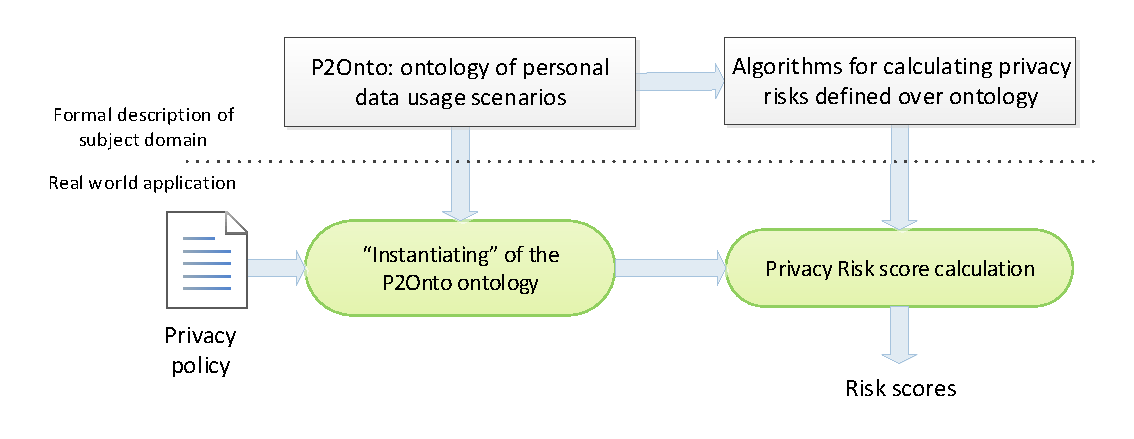
\includegraphics[width=.7\textwidth]{figure1.pdf}}
    \vspace{-\baselineskip}
\end{figure}

Онтология P2Onto призвана обеспечить формальную основу для процедуры оценки риска и может использоваться для проверки и объяснения полученных оценок риска. В нем описываются различные аспекты обработки персональных данных, участвующие в этом процессе субъекты и устанавливаются семантические отношения между ними. Согласно рабочему процессу проектирования онтологий на основе политик конфиденциальности, предложенному в \cite{MDPI8}, построение онтологии требует сначала идентификации основных сценариев использования персональных данных и установления их характеристик, соответствующих задаче анализа. Последнее можно сделать, сформулировав вопросы о компетентности для каждого аспекта конфиденциальности при обработке данных. На рисунке 2 показана схема потока проектирования онтологии P2Onto. 

\begin{figure}[H]
    \centering
    \ffigbox[\FBwidth]
    {\caption{P2Onto процесс проектирования онтологии\label{fig:bow}}}
    {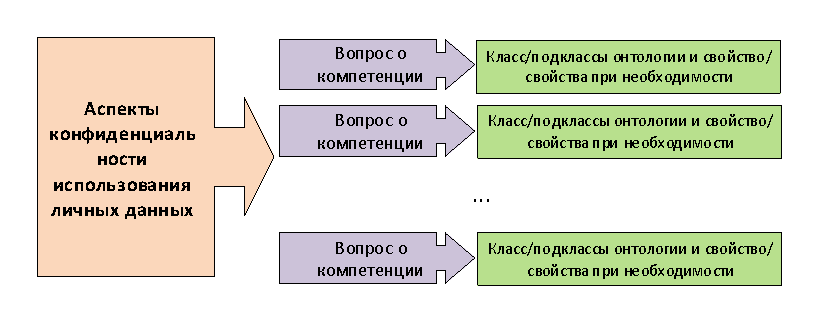
\includegraphics[width=.7\textwidth]{figure2.pdf}}
    \vspace{-\baselineskip}
\end{figure}

За основу были выбраны следующие сценарии и аспекты использования персональных данных:

Собственный сбор и использование данных. Этот аспект характеризует, какие личные данные собирает поставщик услуг, управляя устройством, веб-сайтом или приложением, как они собираются, каковы правовые основания и цели сбора данных.

Сбор и обмен сторонними данными. Этот аспект характеризует все вопросы, касающиеся процедур обмена данными, включая форму обмена данными - агрегированные, анонимные или необработанные.

Безопасность данных. Этот аспект описывает механизмы безопасности, как технические, так и организационные, используемые для защиты данных.

Хранение данных. Этот аспект характеризует временные проблемы обработки и хранения персональных данных.

Агрегация данных. Этот аспект определяет, собирает ли поставщик услуг личные данные.

Настройки конфиденциальности. Эта практика определяет доступные инструменты и варианты для конечного пользователя, чтобы ограничить объем собираемых персональных данных (вопросы согласия / отказа при сборе персональных данных).

Контроль данных. Этот аспект относится к инструментам и механизмам, предоставляемым пользователю для манипулирования личными данными - доступа, редактирования и удаления.

Уведомление о нарушении конфиденциальности. Этот аспект относится к инструментам и механизмам, которые поставщик услуг использует для информирования о нарушении конфиденциальности личных данных.

Изменение политики. Этот аспект относится к тому, какие инструменты и механизмы использует поставщик услуг для информирования конечного пользователя об изменениях в тексте конфиденциальности личных данных и возможных реакциях, доступных конечному пользователю.

Не отслеживать. Эта практика описывает, как обрабатываются сигналы отслеживания для онлайн-отслеживания и рекламы.

Международная и особая аудитория. В этом аспекте обсуждаются различные вопросы, связанные с обработкой персональных данных особой аудитории, такой как дети, и граждане определенных государств и регионов.

Они определены экспертами в предметной области, которые проанализировали существующие политики конфиденциальности и соответствующие правовые нормы и требования, такие как COPPA \cite{MDPI2} и Правило конфиденциальности HIPAA \cite{MDPI3}, и широко используются в исследованиях \cite{MDPI6}, \cite{MDPI18}, \cite{MDPI8}.

Вопросы компетентности к соответствующим аспектам конфиденциальности сценариев использования персональных данных были сформулированы на основе руководящих принципов и анкет, предоставленных международными структурами оценки IoT безопасности, такими как IoTF, GSMA, в области оценки рисков конфиденциальности \cite{MDPI19}, \cite{MDPI20}. Примеры некоторых сценариев использования персональных данных и их проблем с конфиденциальностью с соответствующими вопросами о компетентности и возможными ответами, предоставленными в форме классов онтологий, показаны в таблице 2. Мы ссылались на определения из GDPR, словарей конфиденциальности данных, разработанные W3C Data Privacy Vocabularies и Управляет группой сообщества \cite{MDPI21} другими существующими онтологиями, такими как PROV-O \cite{MDPI22}, \cite{GDPR} чтобы формализовать ответы на вопросы о компетенции и поддерживать единый подход. 

\begin{ltwrap}{2mm}{1.7}{\footnotesize}
    \begin{longtable}[H]{|M{.20\x}|M{.30\x}|M{.50\x}|}
    
        \caption{Сценарии использования персональных данных и вопросы компетенции\label{tab:table2}} \\\hline
        \multicolumn{1}{|H{.20\x}|}{Сценарий использования персональных данных}
        & \multicolumn{1}{H{.30\x}|}{Вопросы о компетенции} 
        & \multicolumn{1}{H{.50\x}|}{Примеры (возможные классы онтологии)}\\\hline
        \endfirsthead
        \caption*{Продолжение таблицы \ref{tab:table2}}\\\hline
        \multicolumn{1}{|H{.20\x}|}{Сценарий использования персональных данных}
        & \multicolumn{1}{H{.30\x}|}{Вопросы о компетенции} 
        & \multicolumn{1}{H{.50\x}|}{Примеры (возможные классы онтологии)}\\\hline
        \endhead
        \endfoot
        \endlastfoot

        First-party data collection and usage
        & Какие категории персональных данных собираются?  
        & Данные учетной записи пользователя, данные устройства, данные приложений, данные о конкретных услугах, финансовая информация, данные отслеживания, конфиденциальные данные и т.д.\\
        
        \cline{2-3}
        
        & Какой режим сбора данных?
        & Автоматически без согласия пользователя, автоматически, но с предоставленным согласием каждый раз, когда выполняется автоматический сбор, например когда пользователь явно разрешает приложению оценивать данные о местоположении или предоставляется пользователем напрямую, когда пользователь совершает платежи\\
        
        \cline{2-3}

        & Какова цель сбора данных? 
        & Предоставление услуг, включая дополнительные услуги, техническую поддержку и поддержку пользователей, аналитику и персонализацию, маркетинг и рекламу, персонализацию, безопасность, требования правовых норм\\
        
        \cline{2-3}

        & Каково основание для сбора данных 
        & Пользователь дал согласие, юридические требования, прочее\\
        
        \cline{2-3}

        & Собираете ли вы данные от сторонних поставщиков услуг?
        & Нет, общедоступные источники, социальные сети, сторонние поставщики услуг и т.д.\\
        
        \cline{2-3}

        & Кто является владельцем данных?
        & Пользователь, другие третьи стороны, например когда собираются данные о членах семьи, гостях\\

        \hline

        First-party data collection and usage
        & Какие категории личных данных передаются?
        & Данные учетной записи пользователя, данные устройства, данные приложений, данные о конкретных услугах, финансовая информация, данные отслеживания, конфиденциальные данные и т.д.\\
        
        \cline{2-3}

        & В каком формате передаются данные?
        & Агрегированные, анонимные, оба, сырые или неопределенные\\
        
        \cline{2-3}

        & Какова цель обмена?
        & Предоставление услуг, включая дополнительные услуги, техническую поддержку и поддержку пользователей, слияние и приобретение, маркетинг и рекламу, персонализацию, безопасность, требования правовых норм и т.д. \\
        
        \cline{2-3}

        & Какова цель распространения?
        & Пользователь дал согласие, юридические требования, прочее\\
        
        \hline

        & Что такое третьи стороны?
        & Аффилированные лица и субподрядчики, юридические лица, другие третьи стороны\\

        \hline

        Data retention
        & Какие категории личных данных сохраняются? 
        & Данные учетной записи пользователя, данные устройства, данные приложений, данные о конкретных услугах, финансовая информация, данные отслеживания, конфиденциальные данные и т.д.\\

        \cline{2-3}
        
        & Какова цель удержания? 
        & Предоставление услуг, включая дополнительные услуги, техническую поддержку и поддержку пользователей, аналитику и персонализацию, маркетинг и рекламу, персонализацию, безопасность, требования правовых норм\\

        \cline{2-3}
        
        & Какова правовая основа удержания? 
        & Пользователь дал согласие, юридические требования, прочее\\

        \cline{2-3}
        
        & Какой срок хранения? 
        & Неопределенный, указанный с явно указанным сроком хранения, неопределенный или другой \\

        \cline{2-3}
        
        & Где они хранятся? 
        & Устройство, облако\\\hline
        
    \end{longtable}
\end{ltwrap}

Тщательный анализ их сценариев использования персональных данных и их аспектов конфиденциальности позволил выделить четыре общих класса - Данные, Действия, Агент и Механизм - которые образуют основу для описания основных сценариев использования персональных данных, остальные классы используются для определения их свойств.

Данные -- это суперкласс, который используется для определения категорий личных и неличных данных. Авторы следуют определению GDPR, чтобы указать типы персональных данных, которые описываются как <<любая информация, относящаяся к идентифицированному или идентифицируемому физическому лицу (<<субъект данных>>); идентифицируемое физическое лицо - это лицо, которое может быть идентифицировано прямо или косвенно, в частности, посредством ссылки на идентификатор, такой как имя, идентификационный номер, данные о местоположении, онлайн-идентификатор или один или несколько факторов, специфичных для физического, физиологическая, генетическая, ментальная, экономическая, культурная или социальная идентичность этого естественного человека>>\cite{MDPI1}, \cite{MDPI4}. Это позволило нам определить такие подклассы персональных данных, как User\_Account\_Data, которые включают информацию о входе в систему, аватар пользователя, электронную почту, физический адрес, User\_Device\_Info и User\_App\_Info, которые содержат данные о пользовательском устройстве и приложениях, такие как версия, модель, время обновления и т. Д., Соответственно. . Мы также обрисовали в общих чертах Tracking\_Data, чтобы указать данные, которые могут использоваться для отслеживания пользователя, такие как IP-адрес, файлы cookie, отпечаток браузера, чтобы иметь возможность оценить сценарий <<Не отслеживать>>, и представили новый подкласс Service\_Data, который используется для указания конкретных данных. для обслуживания и работы устройства, например, блокировки и разблокировки, яркости лампы и т. д., которые могут использоваться для определения привычек и стиля жизни пользователя. Подробная иерархия классов данных, включая иерархию конфиденциальных данных, показана на рисунке 3.

\begin{figure}[H]
    \centering
    \ffigbox[\FBwidth]
    {\caption{Иерархия классов данных\label{fig:bow}}}
    {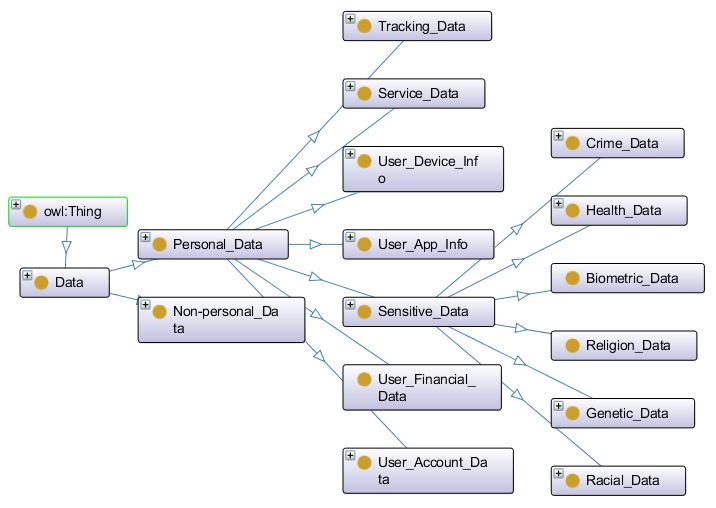
\includegraphics[width=.7\textwidth]{figure3.png}}
    \vspace{-\baselineskip}
\end{figure}

Следует отметить, что класс Non\_Personal\_Data используется для описания неличных данных, возникающих при получении персональных данных посредством анонимизации или агрегации персональных данных. Знание того, сколько типов данных - идентифицируемых и нет - собираются о конкретном пользователе устройства, имеет важное значение в процедуре оценки рисков.

Как следует из списка аспектов конфиденциальности использования персональных данных, некоторые аспекты напрямую связаны с обработкой данных, например сбор, обработка, совместное использование, хранение или безопасность данных первой стороной, в то время как другие относятся к деятельности, которая косвенно связана с обработкой данных. такие как уведомления в случае изменения политики или нарушения данных, предоставление доступа, прав редактирования и стирания и т. д. По этой причине мы выделили два разных подкласса класса активности - Data\_Activity и Control\_Activity. На рисунке 4 показана иерархия подклассов Activity. 

\begin{figure}[H]
    \centering
    \ffigbox[\FBwidth]
    {\caption{Иерархия классов активности\label{fig:bow}}}
    {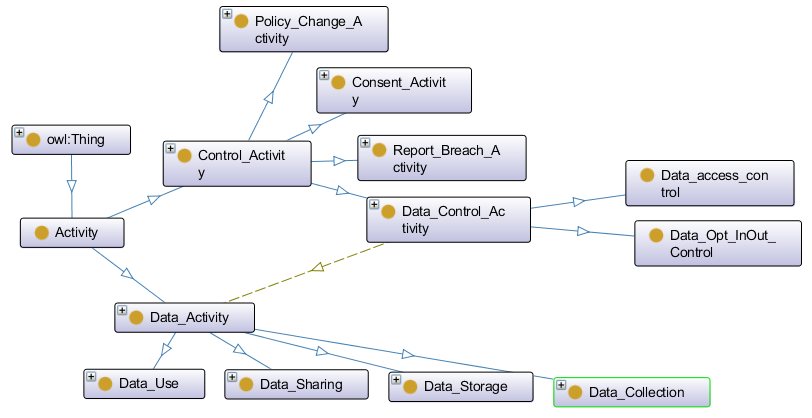
\includegraphics[width=.7\textwidth]{figure4.png}}
    \vspace{-\baselineskip}
\end{figure}

Класс Data\_Activity - это общий класс для определения различных типов операций по обработке данных. Несмотря на то, что эти действия имеют свои отличительные характеристики, можно выделить общие черты, такие как цель операций с данными, формат обрабатываемых данных - анонимные или необработанные, правовая основа для обработки данных и контролирующих лиц. На рисунке 5 показаны наиболее важные классы, относящиеся к деятельности по обработке данных. Цель обработки данных является важной концепцией при оценке рисков конфиденциальности, и мы выделяем следующие цели обработки данных: 1) Предоставление услуг, 2) Реклама и маркетинг 3) Аналитика и исследования, 4) Персонализация, 5) Безопасность, 6) Слияние и поглощение, 7) Соответствие законодательству 8) Другое, 9) Не определено, каждый из них представляет собой отдельный подкласс.

\begin{figure}[H]
    \centering
    \ffigbox[\FBwidth]
    {\caption{Отношения между универсальным классом Data\_Activity и другими классами, характеризующими различные аспекты конфиденциальности\label{fig:bow}}}
    {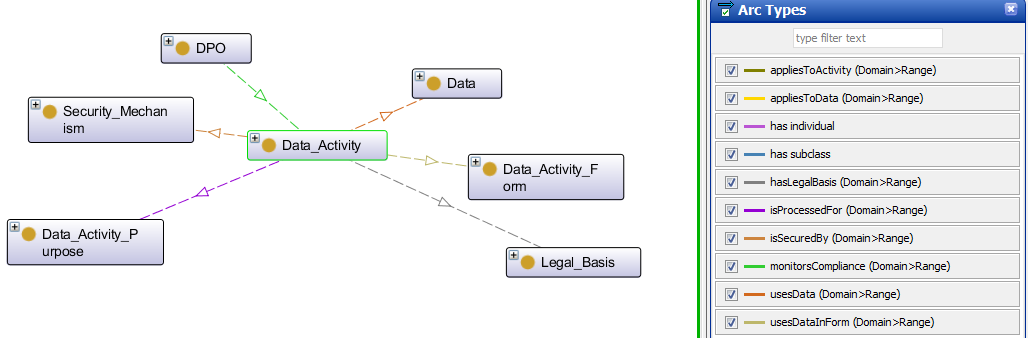
\includegraphics[width=.7\textwidth]{figure5.png}}
    \vspace{-\baselineskip}
\end{figure}

Чтобы указать владельца данных, обработчика данных и ответственного за контроллер данных (DPO), а также других третьих сторон, участвующих в обработке данных, используется класс Agent (рисунок 6). Авторы предлагают повторно использовать эту концепцию из онтологии PROV-O, которая определяет концепт <<Агент>> как субъект, который <<несет некоторую форму ответственности за происходящую деятельность, за существование сущности или за деятельность другого агента>> \cite{MDPI22}. Эта концепция позволяет указать случаи, когда данные собираются от третьих лиц, таких как социальные сети, общедоступные источники с открытым исходным кодом и другие третьи стороны. Он также используется для выявления случаев, когда данные собираются от посторонних лиц, то есть людей, которые не владеют устройством или услугой и с большой вероятностью не дают согласия на обработку данных. 

\begin{figure}[H]
    \centering
    \ffigbox[\FBwidth]
    {\caption{Иерархия классов агентов\label{fig:bow}}}
    {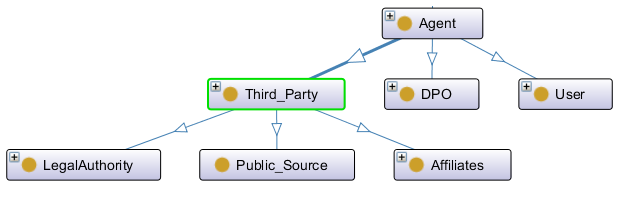
\includegraphics[width=.7\textwidth]{figure6.png}}
    \vspace{-\baselineskip}
\end{figure}

Класс Mechanism - это общий класс, который используется для определения различных инструментов, опций, механизмов и интерфейсов, поддерживающих реализацию различных действий - сбор данных, совместное использование, использование, уведомление в случае изменения политики или нарушения данных. Он используется для характеристики таких свойств, как режим обработки (автоматический или нет), детали реализации деятельности, такие как уведомление по электронной почте или на веб-сайте, доступ к данным через приложение или через конкретный запрос по почте и т. Д.

Все упомянутые выше классы связаны друг с другом с помощью свойств, которые определяют семантические отношения между ними. На рисунке 6 показаны основные концепции и свойства, относящиеся к сценарию использования сохранения данных. Сущности, отмеченные желтыми точками, являются классами, а объекты, отмеченные пурпурным ромбиком, - это отдельные лица, то есть отрывки текста, обнаруженные в политике конфиденциальности. Стрелки соответствуют свойствам, связывающим сущности, их цвет зависит от их типа. Конкретный сценарий, приведенный на Рисунке 7, соответствует сохранению данных для конкретной услуги (износ зубной щетки, оценка производительности и продолжительность чистки), которые хранятся в течение трех месяцев для управления зубной щеткой. Правовая основа для этой деятельности, а также формат хранения данных не были явно упомянуты в тексте, поэтому авторы использовали константу Not Defined для этих классов. 

\begin{figure}[H]
    \centering
    \ffigbox[\FBwidth]
    {\caption{Scenario representing the retention of the service specific data\label{fig:bow}}}
    {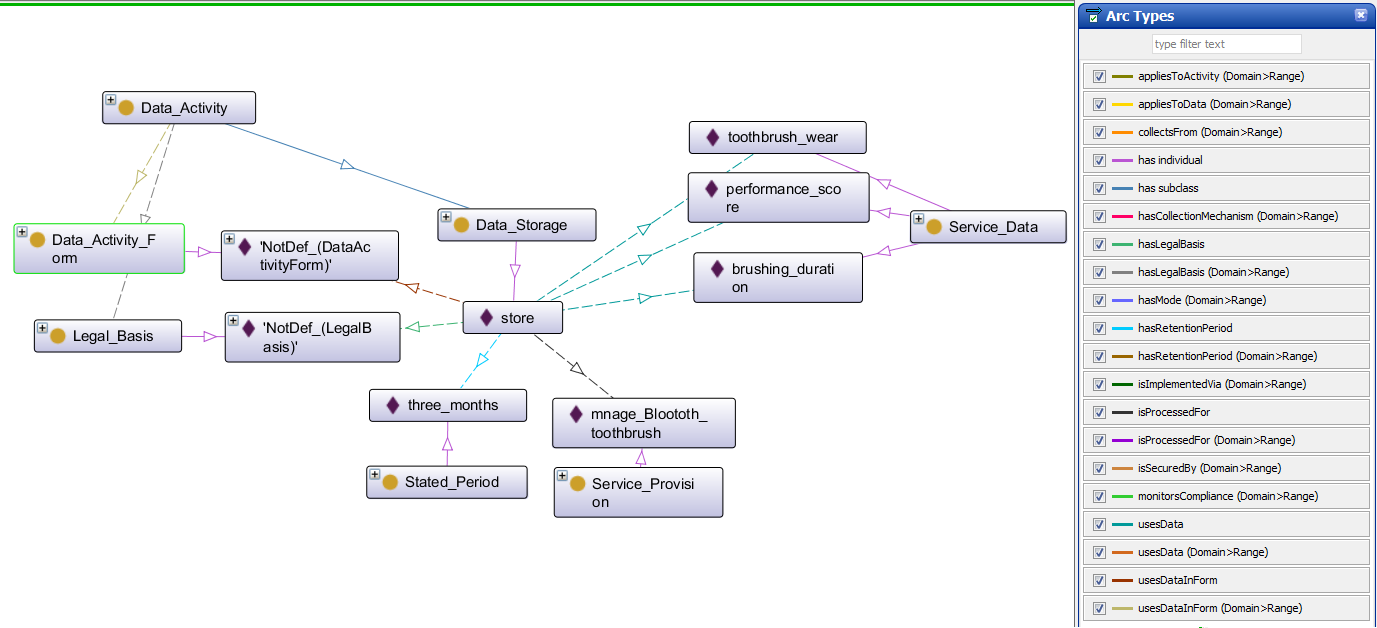
\includegraphics[width=.7\textwidth]{figure7.png}}
    \vspace{-\baselineskip}
\end{figure}

Вопросы о компетенции из раздела 3.1 помогли нам определить основные концепции и свойства онтологии P2Onto.

Алгоритм оценки риска конфиденциальности принимает в качестве входных данных онтологию политики конфиденциальности, описывающую 11 сценариев использования (см. Раздел 3.1).

Основная идея алгоритма заключается в том, что типы персональных данных и их количество определяют основу оценки риска неприкосновенности частной жизни. Другие аспекты, указанные в политике конфиденциальности, такие как цель, правовая основа и варианты подписки / отказа, могут только увеличивать или уменьшать их. Формализующий алгоритм представлен в приложении \hyperref[sec:appendix11]{А.1}.

Расчет оценки риска конфиденциальности RiskScoreBase основан на критичности типов персональных данных и присвоенных им весах, представленных в Таблице 3. Идея алгоритма расчета риска конфиденциальности RiskScoreBase заключается в определении типа персональных данных с наивысшей критичностью. присутствовать в тексте политики конфиденциальности, а затем увеличивать его в зависимости от количества различных типов личных данных. Если в тексте политики присутствуют все типы персональных данных, то риски увеличиваются вдвое. Оценка риска увеличивается логарифмически, чтобы избежать быстрого роста оценки риска. 

\begin{ltwrap}{2mm}{1.7}{\footnotesize}
    \begin{longtable}[H]{|M{.15\x}|M{.3\x}|C{.15\x}|C{.15\x}|}
    
        \caption{Категории персональных данных, их важность и вес\label{tab:table3}} \\\hline
        \multicolumn{1}{|H{.15\x}|}{Классы и подклассы онтологии}
        & \multicolumn{1}{H{.3\x}|}{Категории (класс) } 
        & \multicolumn{1}{H{.15\x}|}{Критичность типа ПД} 
        & \multicolumn{1}{H{.15\x}|}{Влияние категории}\\\hline
        \endfirsthead
        \caption*{Продолжение таблицы \ref{tab:table3}}\\\hline
        \multicolumn{1}{|H{.15\x}|}{Классы и подклассы онтологии}
        & \multicolumn{1}{H{.3\x}|}{Категории (класс) } 
        & \multicolumn{1}{H{.15\x}|}{Критичность типа ПД} 
        & \multicolumn{1}{H{.15\x}|}{Влияние категории}\\\hline
        \endhead
        \endfoot
        \endlastfoot

        Data
        & NonPersonal Data
        & 0
        & 0,0\\
        
        \cline{2-4}

        & Service Data
        & 3
        & 0,9\\
        
        \cline{2-4}

        & Tracking Data
        & 4
        & 1,3\\
        
        \cline{2-4}

        & User Device Data
        & 2
        & 0,4\\
        
        \cline{2-4}

        & App Data
        & 2
        & 0,4\\
        
        \cline{2-4}

        & Sensitive Data
        & 5
        & 2,2\\
        
        \cline{2-4}

        & User Financial Info
        & 4
        & 1,7\\
        
        \cline{2-4}

        & User Account Data
        & 2
        & 0,4\\
        
        \cline{2-4}

        & Other
        & 3
        & 1,3\\
        
        \cline{2-4}

        & Not defined
        & 3
        & 1,3\\\hline
        
    \end{longtable}
\end{ltwrap}

Общая оценка риска на основе анализа онтологии рассчитывается следующим образом: 
\begin{equation}
    \label{eq:formula1}
    PrivacyRiskScore = \sum_i{w_i} \cdot UsageScenarioRiskScore_i, \sum_{i}{w_i} = 1,
\end{equation}
где wi - весовой коэффициент, определяющий влияние оценки риска i-го сценария использования данных. В текущей версии все wi равны друг другу, а общая оценка риска рассчитывается следующим образом: 
\begin{equation}
    \label{eq:formula2}
    PrivacyRiskScore = \frac{1}{n}\sum^n_{i=1}{w_i} \cdot UsageScenarioRiskScore_i,
\end{equation}
где n -- количество анализируемых сценариев использования данных.

Ниже приведен пример расчета риска конфиденциальности для сценария Собственного сбора и использования.

В настоящее время сценарий сбора и использования первой стороной описывается следующими классами и их подклассами: данные (личные данные, неличные данные), правовая основа, цели деятельности с данными. Подклассы этих классов рассматриваются как категории собираемых данных, которые используются в процедуре оценки (см. Таблицу 4). 


\begin{ltwrap}{2mm}{1.7}{\footnotesize}
    \begin{longtable}[H]{|M{.15\x}|M{.3\x}|C{.15\x}|C{.15\x}|}
    
        \caption{Категории целей и правовых оснований сбора персональных данных, их важность и вес\label{tab:table4}} \\\hline
        \multicolumn{1}{|H{.15\x}|}{Классы и подклассы онтологии}
        & \multicolumn{1}{H{.3\x}|}{Категории (класс) } 
        & \multicolumn{1}{H{.15\x}|}{Критичность типа ПД} 
        & \multicolumn{1}{H{.15\x}|}{Влияние категории}\\\hline
        \endfirsthead
        \caption*{Продолжение таблицы \ref{tab:table4}}\\\hline
        \multicolumn{1}{|H{.15\x}|}{Классы и подклассы онтологии}
        & \multicolumn{1}{H{.3\x}|}{Категории (класс) } 
        & \multicolumn{1}{H{.15\x}|}{Критичность типа ПД} 
        & \multicolumn{1}{H{.15\x}|}{Влияние категории}\\\hline
        \endhead
        \endfoot
        \endlastfoot

        Purpose
        & Service Provision 
        & 1
        & 0,0\\
        
        \cline{2-4}

        & Security Purpose
        & 1
        & 0,0\\
        
        \cline{2-4}

        & Analytics Personalization
        & 3
        & 2,3\\
        
        \cline{2-4}

        & Adverising Marketing
        & 3
        & 2,3\\
        
        \cline{2-4}

        & Merge Acqisition
        & 2
        & 1,5\\
        
        \cline{2-4}

        & Other
        & 1
        & 1,3\\
        
        \cline{2-4}

        & NotDef*
        & 4
        & 3,0\\

        \hline

        Legal Basis
        & Consent
        & 0
        & 0,0\\
        
        \cline{2-4}

        & Legal requirement
        & 0,0
        & 1,7\\
        
        \cline{2-4}

        & Other
        & 1,5
        & 1,7\\
        
        \cline{2-4}

        & NotDef*
        & 0,0
        & 3,0\\\hline
        
    \end{longtable}
\end{ltwrap}

Критичность каждой категории в таблице 4 присвоена в соответствии с экспертными знаниями. Для целей и юридических оснований десятичный логарифм максимального веса дает 1,77, чтобы увеличить оценку по данным в 1,77 раза, если две категории имеют высокую критичность, и 1,47, если только одна категория имеет высокую критичность.

Алгоритм оценки риска сценария использования первой стороной (FP\_RiskScore):

Авторы сначала рассчитывают базу оценок рисков конфиденциальности RiskScoreBase на основе критичности личных данных, упомянутых в сценарии использования данных. Этот алгоритм похож для разных сценариев использования.

Пусть PD\_classi - это категория личных данных, как определено в таблице 3. Это возвращается функцией getCategory () из алгоритма выше.

Пусть PD\_Criticalityi - это критичность i-й категории персональных данных.

Пусть max\_criticality - это максимальная критичность среди критичностей категорий данных, не пустых в онтологии. Это возвращается функцией getMaxCritCat () из алгоритма выше. Формализующий алгоритм представлен в приложении \hyperref[sec:appendix12]{А.2}.

В дальнейшем мы можем увеличивать или уменьшать эту оценку риска на основе критичности категорий онтологии других классов. 

Пусть P\_classi - это категория цели использования личных данных, как определено в Таблице 4, а LB\_classi - категория правовой основы для использования личных данных. Это возвращается функцией getCategory() из алгоритма выше. 

Пусть P\_Criticalityi - критичность i-й категории (подкласса) P\_classi, LB\_Criticalityi - критичность i-й категории LB\_classi.

Пусть max\_P\_Criticality - это максимальная критичность среди критичностей целей использования данных, которые не пусты в онтологии, а max\_LB\_Criticality - максимальная критичность среди критичностей правовой основы для использования данных, которые не пусты в онтологии. Это возвращается функцией getMaxCritCat() из алгоритма выше. 

Пусть P\_weight - это вес для целевой категории с max\_P\_Criticality, а LB\_weight - вес для юридической категории с max\_LB\_Criticality. Это возвращается функцией getClassWeight() из алгоритма выше. Формализующий алгоритм представлен в приложении \hyperref[sec:appendix13]{А.3}.

Фактически, чтобы снизить FP\_RiskScore, необходимо манипулировать весами Цели и Правовой основы. 

Для оценки предложенного подхода авторы выбрали четыре политики конфиденциальности, написанные для разных типов сервисов и устройств. Все политики конфиденциальности, за исключением августовской политики конфиденциальности, были выбраны из набора данных OPP-115 \cite{MDPI23}, который был создан в 2016 году. Вот почему политики конфиденциальности устарели, и, безусловно, текущие версии политик конфиденциальности компаний содержат всю информацию, необходимую для соответствовать законодательным требованиям GDPR \cite{GDPR}, CCPA \cite{MDPI23}, COPPA \cite{MDPI2}. Выбор этих политик объясняется тем, что они представляют различные типы сервисов и имеют аннотации, которые помогают проверять результаты и сущности онтологии. 



\begin{ltwrap}{2mm}{1.7}{\footnotesize}
    \begin{longtable}[H]{|M{.2\x}|M{.2\x}|M{.6\x}|}
    
        \caption{Описание политик конфиденциальности\label{tab:table5}} \\\hline
        \multicolumn{1}{|H{.2\x}|}{Company name}
        & \multicolumn{1}{H{.2\x}|}{Privacy policy} 
        & \multicolumn{1}{H{.6\x}|}{Brief description of company activity}\\\hline
        \endfirsthead
        \caption*{Продолжение таблицы \ref{tab:table5}}\\\hline
        \multicolumn{1}{|H{.2\x}|}{Company name}
        & \multicolumn{1}{H{.2\x}|}{Privacy policy} 
        & \multicolumn{1}{H{.6\x}|}{Brief description of company activity}\\\hline
        \endhead
        \endfoot
        \endlastfoot

        August Products \& Services
        & 24 July 2020 
        & It is a company that produces devices for smart home, such as smart locks, doorbell cameras and other accesso-ries [25]. Their smart lock allows implementing a variety of convenient but privacy risky functions as remotely lock and unlock the door, logging exit/entrance activity of smart lock owners as well as their guests, supports biometrical identi-fication and voice assistant.\\

        \hline

        Ticketmaster website
        & July 20, 2012
        & It is online service of the world entertainment company that organizes different live events for well-known and emerging artists. Their online service allows choosing any entertain-ment event and buying tickets for it, that it is expected that the risks for this policy could be rather high as it should deal with users’ financial data.\\

        \hline

        Cincinnati Museum Center
        & September 09, 2011
        & This privacy policy belongs to the cultural center that unites three museums with different exhibits, organizes different events including one for children with possibility to book them in advance. Like in previous case it is ex-pected to have quite high risks due to processing financial data.\\

        \hline
        
        Instagram 
        & January 19, 2013
        & This privacy policy belongs to a popular public social net-work targeted primary for sharing photo and video data. Till 2019 there were no possibilities for online shopping via Instagram.\\\hline
        
    \end{longtable}
\end{ltwrap}

Авторы сосредоточились на трех аспектах использования данных: сбор и использование данных собственными силами, сбор и обмен данными сторонними организациями и хранение данных для сравнения полученных оценок рисков. Другие аспекты конфиденциальности не были охвачены всеми политиками конфиденциальности. Например, продукты августа не предназначены для использования несовершеннолетними до 16 лет, сервисы Instagram и Ticket-master не предназначены для детей младше 13 лет, поэтому риски конфиденциальности для этой конкретной аудитории не рассчитываются. Также следует отметить, что сценарий использования, описывающий уведомление о нарушении конфиденциальности, не был обнаружен в текстах всех политик конфиденциальности. Политика конфиденциальности Cincinatti Museum не содержит информации о хранении Данных. Необходимо отметить, что текущая версия политики конфиденциальности музеев также содержит минимум информации о хранении данных и очень расплывчата.

В большинстве случаев политики конфиденциальности носят общий характер, во многих сценариях использования данных отсутствует информация об определенных аспектах конфиденциальности. Если эта информация не указана явно, она помечается как <<Не определено>>. Оказалось, что эта концепция присутствует практически во всех сценариях использования персональных данных. С одной стороны, его можно использовать для характеристики прозрачности политики - чем больше число соответствующих лиц, тем более расплывчатая и неясная политика. С другой стороны, он имеет самый высокий вес в процедуре оценки риска, и интересно понять, как он влияет на общие оценки риска. Поэтому в экспериментах авторы проводили расчет для обоих случаев, учитывая категорию Not Defined для каждого класса и игнорируя ее.

Таблица 6 содержит оценки, полученные для каждого сценария личного использования. Рассчитанные оценки рисков вполне естественны и легко объяснимы. Политика конфиденциальности Instagram имеет самую низкую RiskScoreBase почти во всех сценариях использования данных, это объясняется тем, что объем собираемых персональных данных минимален, компания не собирает никаких чувствительных и финансовых данных, однако риски довольно высоки. объясняется непрозрачностью целей, обратите внимание, что оценка риска снижается, когда категория <<Не определено>> не рассматривается. Остальные политики имеют сопоставимую базу данных RiskScoreBase, потому что они собирают почти все типы персональных данных, кроме конфиденциальной. Августовская интеллектуальная блокировка также собирает некоторую служебную информацию, такую ​​как статус блокировки, информацию о пользователях блокировки. Как и в политике Instagram, высокие риски в большинстве случаев объясняются наличием концепции Not Defined. Однако для Музейного центра Цинциннати эти риски сохраняются даже тогда, когда в расчетах не учитывается концепция Неопределенного. При этом поясняется, что Центр делится почти всеми данными с неопределенными или неназванными третьими сторонами. Высокие риски хранения августовского смарт-замка объясняются наличием неограниченного срока хранения данных. Однако, когда авторы этого исследования подробно изучили эту политику, они обнаружили, что эта информация относится только к личным данным в агрегированной форме. 

\begin{ltwrap}{2mm}{1.7}{\footnotesize}
    \begin{longtable}[H]{|M{.15\x}|M{.28\x}|C{.1475\x}|C{.1475\x}|C{.1475\x}|C{.1475\x}|}
    
        \caption{Присвоенные ранги P2Onto лицам для разных концепций\label{tab:table6}} \\\hline
        \multicolumn{1}{|H{.15\x}|}{Data Usage Scenario}
        & \multicolumn{1}{H{.28\x}|}{Risk scores} 
        & \multicolumn{1}{H{.1475\x}|}{August Products \& Services} 
        & \multicolumn{1}{H{.1475\x}|}{Ticketmaster website} 
        & \multicolumn{1}{H{.1475\x}|}{Cincinnati Museum Center}
        & \multicolumn{1}{H{.1475\x}|}{Instagram}\\\hline
        \endfirsthead
        \caption*{Продолжение таблицы \ref{tab:table6}}\\\hline
        \multicolumn{1}{|H{.15\x}|}{Data Usage Scenario}
        & \multicolumn{1}{H{.28\x}|}{Risk scores} 
        & \multicolumn{1}{H{.1475\x}|}{August Products \& Services} 
        & \multicolumn{1}{H{.1475\x}|}{Ticketmaster website} 
        & \multicolumn{1}{H{.1475\x}|}{Cincinnati Museum Center}
        & \multicolumn{1}{H{.1475\x}|}{Instagram}\\\hline
        \endhead
        \endfoot
        \endlastfoot

        \multirow{2}{=}{First Party Collection and Use}
        & RiskScoreBase\newline(with Not Def category)
        & 7,08
        & 6,55
        & 6,55
        & 4,50\\

        \cline{2-6}
        
        & RiskScoreBase\newline(without Not Def category)
        & 6,55
        & 6,55
        & 5,93
        & 3,78\\

        \cline{2-6}
        
        & UsageScenarioRiskScore\newline(with Not Def category)
        & 9,82
        & 9,84
        & 9,65
        & 8,01\\

        \cline{2-6}
        
        & UsageScenarioRiskScore\newline(without Not Def category)
        & 9,67
        & 9,74
        & 9,37
        & 5,96\\
        
        \hline

        Third Party Sharing
        & RiskScoreBase\newline(with Not Def category)
        & 4,24
        & 3,34
        & 6,55
        & 4,50\\

        \cline{2-6}
        
        & RiskScoreBase\newline(without Not Def category)
        & 3,34
        & 3,00
        & 5,93
        & 3,78\\

        \cline{2-6}
        
        & UsageScenarioRiskScore\newline(with Not Def category)
        & 8,55
        & 6,27
        & 9,65
        & 8,67\\

        \cline{2-6}
        
        & UsageScenarioRiskScore\newline(without Not Def category)
        & 5,95
        & 4,96
        & 9,37
        & 6,92\\
        
        \hline

        Data retention
        & RiskScoreBase\newline(with Not Def category)
        & 6,37
        & 3,34
        & --
        & 3,40\\

        \cline{2-6}
        
        & RiskScoreBase\newline(without Not Def category)
        & 5,66
        & 3,00
        & --
        & 1,30\\

        \cline{2-6}
        
        & UsageScenarioRiskScore\newline(with Not Def category)
        & 9,82
        & 5,95
        & --
        & 6,62\\

        \cline{2-6}
        
        & UsageScenarioRiskScore\newline(without Not Def category)
        & 9,67
        & 4,96
        & --
        & 2,61\\\hline
        
    \end{longtable}
\end{ltwrap}

Анализ политики с использованием онтологии выявил много интересных вопросов. Например, смарт-замок собирает данные от гостей, которые посещают своего владельца, это делается для того, чтобы предоставить доступ смарт-замку и организовать процесс приглашения. На рисунке 8 показан этот конкретный сценарий использования данных.

\begin{figure}[H]
    \centering
    \ffigbox[\FBwidth]
    {\caption{Часть онтологии P2Onto, представляющая практику использования данных для сбора данных первой стороной, обнаруженную в августовской политике конфиденциальности\label{fig:bow}}}
    {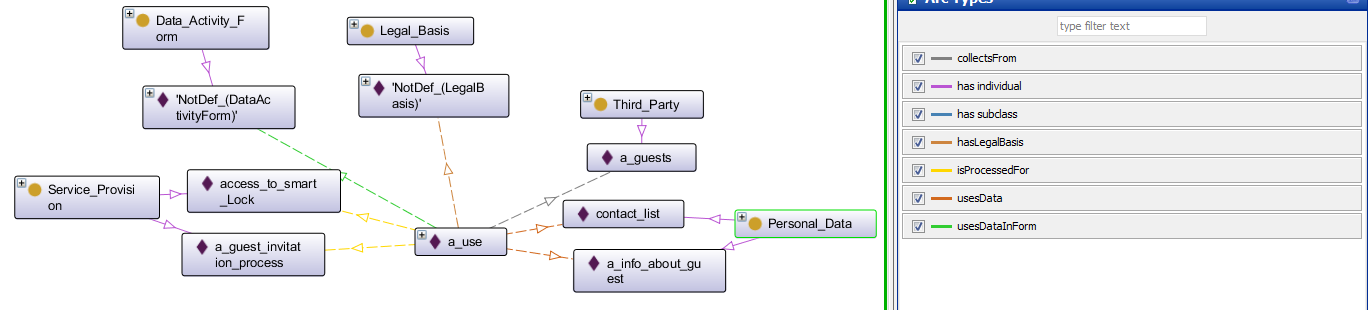
\includegraphics[width=.7\textwidth]{figure8.png}}
    \vspace{-\baselineskip}
\end{figure}

На рисунке 9 показан сценарий совместного использования данных. Хотя данные передаются третьим лицам в аналитических и маркетинговых целях, формат обмена данными сохраняет конфиденциальность владельца данных.

Это заставило авторов сделать вывод о необходимости учитывать в процедуре расчета риска каждый конкретный сценарий использования данных. И требуется найти баланс между Неопределенными категориями, которые бы в них присутствовали. Применение онтологии в качестве основы для построения таких правил допускает эти изменения, поскольку все сценарии данных представлены как связанные концепции онтологии. Эта способность онтологии также полезна для объяснения полученных результатов, поскольку ясно, как различные типы персональных данных собираются, обрабатываются и передаются, какие инструменты и опции для доступа, редактирования персональных данных или их удаления доступны конечному пользователю. , так далее.

\begin{figure}[H]
    \centering
    \ffigbox[\FBwidth]
    {\caption{Часть онтологии P2Onto, представляющая практику хранения данных, обнаруженную в августовской политике конфиденциальности\label{fig:bow}}}
    {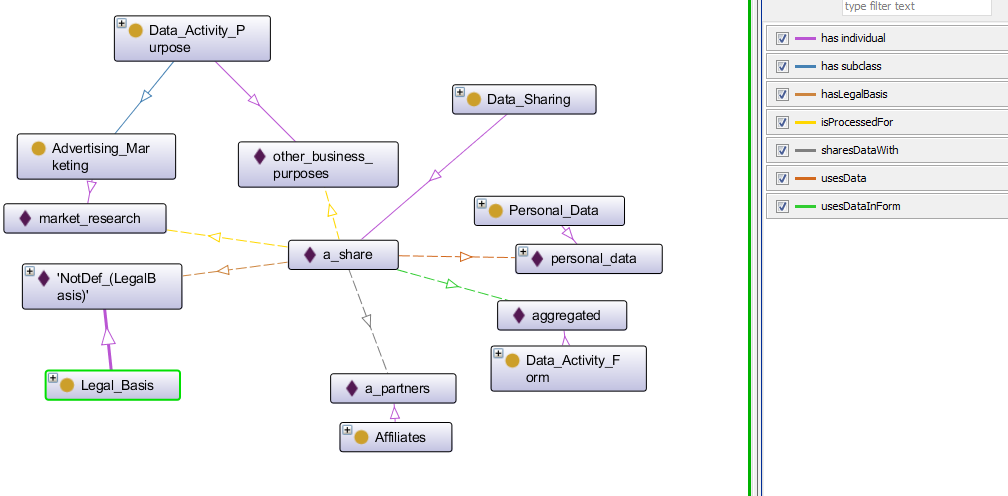
\includegraphics[width=.7\textwidth]{figure9.png}}
    \vspace{-\baselineskip}
\end{figure}

Авторы считают, что эта онтология может служить основой для разработки интерактивных моделей визуализации на основе графов, нацеленных на объяснение рисков конфиденциальности для конечного пользователя в ясной и удобочитаемой форме. 

\subsection{Заключение}
Конфиденциальность в настоящее время вызывает растущую озабоченность. Для защиты конфиденциальности пользователей было разработано множество стандартов. Они обязывают организации четко указывать в политиках конфиденциальности, какие личные данные они используют, для каких целей, кем и как долго. Текст политики конфиденциальности может ввести пользователей в заблуждение. В этой статье авторы предложили подход к оценке частных рисков на основе онтологии, чтобы сделать понятным и прозрачным для пользователя, какие риски конфиденциальности могут возникать в результате политики конфиденциальности.

Разработанный подход основан на анализе политики конфиденциальности. Он включает в себя анализ текстов политики конфиденциальности, представленных на естественном языке, с использованием сначала методов обработки на естественном языке, генерацию и обработку онтологии политики конфиденциальности для каждой политики, указанной на естественном языке, и вычисление рисков конфиденциальности с использованием созданной онтологии. Предлагаемая онтология политики конфиденциальности, описывающая различные сценарии использования данных, является ядром разработанного подхода. Процесс создания онтологии основан на вопросах компетентности для каждого аспекта конфиденциальности операций по обработке данных, которые позволяют идентифицировать основные сценарии использования персональных данных и устанавливать их характеристики, соответствующие задаче анализа. В статье авторы описали разработанный процесс генерации онтологий, общую онтологию политик конфиденциальности и примеры фрагментов онтологий для конкретных политик.

Также авторы описали разработанный алгоритм расчета рисков конфиденциальности на основе сгенерированной онтологии. Основная идея алгоритма заключается в том, что типы персональных данных и их количество определяют основу оценки риска неприкосновенности частной жизни. Другие аспекты, указанные в политике конфиденциальности, такие как цель, правовая основа и варианты подписки / отказа, могут только увеличивать или уменьшать их.
Этот подход демонстрируется в нескольких политиках конфиденциальности. Описаны и проанализированы проведенные эксперименты. Они продемонстрировали применимость подхода для представления основных аспектов использования данных в ясной и удобочитаемой форме и для объяснения рассчитанной оценки риска.

Кроме того, эксперименты показали, что установление рангов для людей - важный аспект, требующий дополнительных исследований. Еще одно важное направление будущих исследований связано с автоматизацией обнаружения концептов онтологии в тексте политики с использованием методов обработки естественного языка. 



\subsection{Постановка задачи}
Текст\dots

\newpage
\section{Применение строгих методов анализа текста для формализации политик безопасности}

\subsection{Статистические модели текстовых документов}

Были протестированы две модели векторизованного представления текста -- <<мешок слов>> и модель TF-IDF. Модель <<мешок слов>> представляет документ в виде матрицы, представленной на рисунке \ref{fig:bow}. Здесь слова каждого абзаца подсчитываются и сопоставляются с абзацами, в которых они встретились.

\begin{figure}[H]
    \centering
    \ffigbox[\FBwidth]
    {\caption{Bag-of-Words матрица\label{fig:bow}}}
    {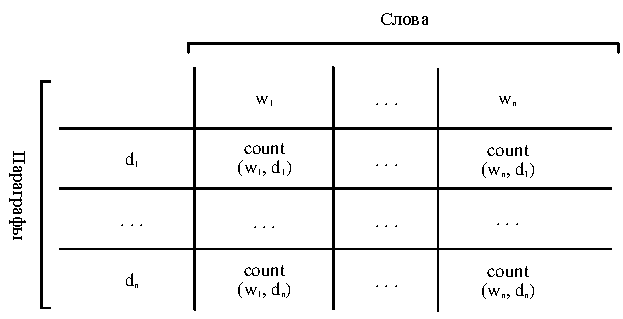
\includegraphics[width=.7\textwidth]{bow.pdf}}
    \vspace{-\baselineskip}
\end{figure}


Модель TF-IDF представляет документ в виде матрицы, представленной на рисунке \ref{fig:tfidf}. Формула (\ref{eq:tfidf}) показывает, как можно получить метрику TF-IDF.
\begin{equation}
    \label{eq:tfidf}
    tfidf(t, d, D) = \frac{n_t}{\displaystyle\sum_k n_k} \times 
    log \frac{ \big|{D}\big| }
    { \big|\left\{ d_i \in D : t \in d_i \right\}\big| }\ ,
\end{equation}
\makebox[12.5mm]{где\hfill}$t$ -- термин или слово;\\
\makebox[12.5mm]{}$d$ -- конкретный абзац;\\
\makebox[12.5mm]{}$D$ -- набор абзацев. 

Итак, модель TF-IDF придает больший вес словам которые использованы меньше раз. Это может быть полезно, когда тексты схожи с точки зрения используемых слов, как в нашем случае, для политик безопасности.

\begin{figure}[H]
    \centering
    \ffigbox[\FBwidth]
    {\caption{Матрица TF-IDF\label{fig:tfidf}}}
    {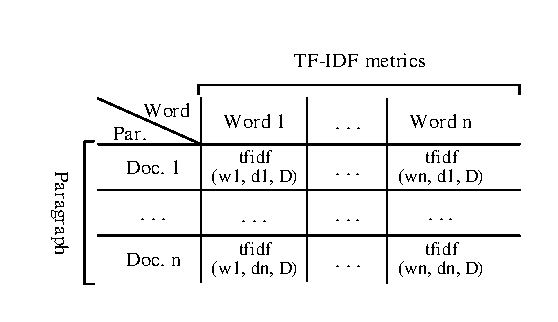
\includegraphics[width=.7\textwidth]{tfidf.pdf}}
    \vspace{-\baselineskip}
\end{figure}

\subsection{Подход основанный на латентно-семантическом анализе текста}

Современные методы кластеризации текстов позволяют определять тематику текстов с высокой точностью. Однако большинство из этих методов принимают тексты с самыми разными темами как вход для алгоритмов. Но тексты со схожими тематиками можно проанализировать с помощью ла\-тен\-тно-семантического анализа дважды: группировать тексты по темам один раз, и предоставить еще более детальное разделение их по подтемам во второй раз. Такой подход можно использовать для более точной классификации абзацев с точки зрения их характеристик и аспектов использования персональных данных. Следует отметить, что латентно-семантический поиск сильно зависит от глобального текстового контекста с потерями информации о локальных контекстных отношениях между словами. Были выделены девять тем конфиденциальности, которые следует сопоставить с абзацами согласия пользователя сайта -- <<сбор личных данных>>, <<сбор данных третьими лицами>>, <<управление личными данными>>, <<механизмы защиты персональных данных>> и др. Очевидно, что аспекты обращения с данными состоят из нескольких слов, и в некоторых случаях перекрываются. На основании этих фактов была выдвинута гипотеза о том, что латентно-семантический поиск способен обнаружить даже незначительную разницу в тексте абзацев при пропуске частых слов. Перед применением латентно-семантического анализа требуется предварительная обработка входных данных. Обычно эта процедура включает очистку данных, удаление гиперссылок, пунктуации и т. д. Также текст политик конфиденциальности был разбит на набор абзацев. Каждый абзац был преобразован в массив слов, которые он содержит. Следующим шагом было удаление наиболее частых, но не столь значимых слов, так называемых стоп-слов. Также была применена операция стемминга, чтобы рассматривать только основную часть всех слов полученных от единого корня.

Пусть A -- это матрица абзацев и слов, тогда используя формулу (\ref{eq:lsa})
\begin{equation}
    \label{eq:lsa}
    A = U \times S \times V^T,
\end{equation}
\makebox[12.5mm]{где\hfill}$A$ -- матрица слов и параграфов;\\
\makebox[12.5mm]{\hfill}$U$ -- ортонормированная матрица $U$;\\
\makebox[12.5mm]{\hfill}$V$ -- ортонормированная матрица $V$;\\
\makebox[12.5mm]{\hfill}$S$ -- диагональная матрица $S$, значения которой сингулярны для $A$.

После того, как матрица была разделена на три компонента, матрица $U$ содержит $n$-мерные векторы, которые можно интерпретировать как координаты в $n$-мерном пространстве \cite{LSA}. Документы могут быть распределены по кластерам по значениям этих координат. Проведенные эксперименты с латентно-семантическим анализом выполнялись с использованием набора данных с открытым исходным кодом, который включает 115 политик безопасности, которые были размечены вручную, и все абзацы присвоены одному или нескольким сценариям использования персональных данных \cite{OPP}. Результаты экспериментов для модели <<мешок слов>> представлены в таблице \ref{tab:clusters1}, в ней показаны полученные кластеры и соответствующие значения координат.

\begin{ltwrap}{2mm}{1.7}{\footnotesize}
    \begin{longtable}[H]{|C{.05\x}|M{.2\x}|M{.2\x}|M{.2\x}|M{.2\x}|}
        \caption{Кластеры политик безопасности для модели Bag-of-Words\label{tab:clusters1}}\\\hline
        \multicolumn{1}{|H{.05\x}|}{№}
        & \multicolumn{1}{H{.2\x}|}{Координата 1} 
        & \multicolumn{1}{H{.2\x}|}{Координата 2} 
        & \multicolumn{1}{H{.2\x}|}{Координата 3} 
        & \multicolumn{1}{H{.2\x}|}{Координата 4}\\\hline
        \endfirsthead
        \caption*{Продолжение таблицы \ref{tab:clusters1}}\\\hline
        \multicolumn{1}{|H{.05\x}|}{№}
        & \multicolumn{1}{H{.2\x}|}{Координата 1} 
        & \multicolumn{1}{H{.2\x}|}{Координата 2} 
        & \multicolumn{1}{H{.2\x}|}{Координата 3} 
        & \multicolumn{1}{H{.2\x}|}{Координата 4}\\\hline
        \endhead
        \endfoot
        \endlastfoot
        0 & 0.634”inform”  & 0.28”may”        & 0.276”use”     & 0.232”servic”   \\\hline
        1 & 0.202“cooki”   & 0.466“inform”    & 0.336“site”    & 0.257“use”      \\\hline
        2 & 0.524“privaci” & 0.433“polici”    & 0.388“cooki”   & 0.219“site”     \\\hline
        3 & -0.589“servic” & 0.344“site”      & 0.244“parti”   & -0.240“third”   \\\hline
        4 & -0.504“parti”  & 0.486 “third”    & -0.449“servic” & 0.235“advertis” \\\hline
        5 & -0.594“site”   & 0.278“cooki”     & 0.272“websit”  & 0.264“privaci”  \\\hline
        6 & -0.326“may”    & 0.311“site”      & 0.307“servic”  & -0.293”email”   \\\hline
        7 & -0.437”may”    & -0.369”advertis” & 0.345”person”  & 0.319”cooki”    \\\hline
        8 & 0.501”may”     & -0.315”email”    & -0.281”use”    & -0.264”address” \\\hline
        9 & -0.488”user”   & -0.384”use”      & 0.310”provid”  & -0.301”websit”  \\\hline
    \end{longtable}
\end{ltwrap}

Как видно, результаты противоречивы, поэтому трудно понять, какая из тем каким смыслом обладает. Затем рассчитывалась метрика принадлежности к теме с помощью библиотеки Gensim \cite{Gensim} и результаты снова не были обнадеживающими. Результаты расчета метрики принадлежности кластеру представлены в таблице \ref{tab:affiliation_bow1}.

\begin{ltwrap}{2mm}{1.7}{\footnotesize}
    \begin{longtable}[H]{|M{.13\x}|C{.1\x}|C{.1\x}|C{.1\x}|C{.1\x}|C{.1\x}|}
        \caption{Принадлежность кластерам\label{tab:affiliation_bow1}}\\\hline
        \endfirsthead
        \caption*{Продолжение таблицы \ref{tab:clusters1}}\\\hline
        \endhead
        \endfoot
        \endlastfoot
        Topic       & 0     & 1     & 2    & 3     & 4     \\\hline
        Affiliation & 2.27  & -0.8  & 0.15 & -0.22 & -1.2  \\\hline
        Topic       & 5     & 6     & 7    & 8     & 9     \\\hline
        Affiliation & -0.17 & -0.15 & -0.2 & 0.22  & -0.07 \\\hline
    \end{longtable}
\end{ltwrap}

Другие результаты с параграфами, относящимися к другому аспекту обращения с данными, были почти такими же. Результаты
представлены в таблице \ref{tab:affiliation_bow2}.

\begin{ltwrap}{2mm}{1.7}{\footnotesize}
    \begin{longtable}[H]{|M{.13\x}|C{.1\x}|C{.1\x}|C{.1\x}|C{.1\x}|C{.1\x}|}
        \caption{Принадлежность кластерам\label{tab:affiliation_bow2}}\\\hline
        \endfirsthead
        \caption*{Продолжение таблицы \ref{tab:clusters1}}\\\hline
        \endhead
        \endfoot
        \endlastfoot
        Topic       & 0    & 1     & 2    & 3    & 4    \\\hline
        Affiliation & 2.59 & -0.76 & 0.64 & 0.74 & 0.13 \\\hline
        Topic       & 5    & 6     & 7    & 8    & 9    \\\hline
        Affiliation & 0.14 & -0.12 & 0.23 & 0.12 & 0.41 \\\hline
    \end{longtable}
\end{ltwrap}

Все протестированные абзацы были сопоставлены с кластером 0, что не может быть верным так как абзацы относились к заведомо разным аспектам обращения с персональными данными. 

Результаты экспериментов для модели TF-IDF представлены далее, в таблице \ref{tab:clusters2}. Также показывались десять кластеров и значения атрибутов. И, как в первом случае с <<мешком слов>>, по значениям координат невозможно судить о теме кластера.

\begin{ltwrap}{2mm}{1.7}{\footnotesize}
    \begin{longtable}[H]{|C{.05\x}|M{.2\x}|M{.2\x}|M{.2\x}|M{.2\x}|}
        \caption{Кластеры политик безопасности для модели TF-IDF\label{tab:clusters2}}\\\hline
        \multicolumn{1}{|H{.05\x}|}{№}
        & \multicolumn{1}{H{.2\x}|}{Координата 1} 
        & \multicolumn{1}{H{.2\x}|}{Координата 2} 
        & \multicolumn{1}{H{.2\x}|}{Координата 3} 
        & \multicolumn{1}{H{.2\x}|}{Координата 4}\\\hline
        \endfirsthead
        \caption*{Продолжение таблицы \ref{tab:clusters2}}\\\hline
        \multicolumn{1}{|H{.05\x}|}{№}
        & \multicolumn{1}{H{.2\x}|}{Координата 1} 
        & \multicolumn{1}{H{.2\x}|}{Координата 2} 
        & \multicolumn{1}{H{.2\x}|}{Координата 3} 
        & \multicolumn{1}{H{.2\x}|}{Координата 4}\\\hline
        \endhead
        \endfoot
        \endlastfoot
        0 & 0.202“cooki”     & 0.2“may”        & 0.198“inform”   & 0.198“site”     \\\hline
        1 & 0.573“cooki”     & 0.262“browser”  & 0.195“advertis” & 0.182“web”      \\\hline
        2 & -0.406“media”    & 0.291“cooki”    & 0.282“health”   & 0.279“advertis” \\\hline
        3 & -0.453“health”   & 0.258“email”    & -0.204“kaleida” & 0.191“address”  \\\hline
        4 & 0.423“health”    & 0.215“media”    & 0.205“kaleida”  & -0.199“secur”   \\\hline
        5 & -0.299“advertis” & 0.262“health”   & -0.252“media”   & -0.213“privaci” \\\hline
        6 & -0.325“media”    & 0.263“polici”   & 0.249“privaci”  & 0.197”chang”    \\\hline
        7 & 0.280”cooki”     & -0.216”device”  & -0.183”health”  & -0.166”social”  \\\hline
        8 & -0.223”advertis” & -0.206”teenag”  & -0.206”inelig”  & 0.176”child”    \\\hline
        9 & -0.263” child”   & -0.26”wireless” & 0.245”message”  & 0.239”parent”   \\\hline
    \end{longtable}
\end{ltwrap}

Результаты кластеризации снова противоречивы, поэтому трудно сказать, какая конкретная тема описывает какой аспект политики конфиденциальности. В разных темах встречаются одни и те же слова с изменение веса. Для аспектов политики конфиденциальности, которые мы искали нет тем, которые могли бы их точно описать, поскольку многие из них могут. Затем с помощью библиотеки Gensim был рассчитан показатель принадлежности к теме, и результаты снова не были обнадеживающими. Результаты расчета аффилированности по абзацу одной из политик конфиденциальности представленные в таблице \ref{tab:affiliation_tfidf1}.

\begin{ltwrap}{2mm}{1.7}{\footnotesize}
    \begin{longtable}[H]{|M{.13\x}|C{.1\x}|C{.1\x}|C{.1\x}|C{.1\x}|C{.1\x}|}
        \caption{Принадлежность кластерам\label{tab:affiliation_tfidf1}}\\\hline
        \endfirsthead
        \caption*{Продолжение таблицы \ref{tab:affiliation_tfidf1}}\\\hline
        \endhead
        \endfoot
        \endlastfoot
        Topic       & 0    & 1     & 2     & 3     & 4     \\\hline
        Affiliation & 2.18 & -0.97 & -0.69 & -0.27 & 0.65  \\\hline
        Topic       & 5    & 6     & 7     & 8     & 9     \\\hline
        Affiliation & 0.98 & -1.17 & 0.8   & 0.27  & 0.01  \\\hline
    \end{longtable}
\end{ltwrap}

Результат для другого абзаца, относящегося к другой политике конфиденциальности, был почти такой же. Результаты представлены в таблице \ref{tab:affiliation_tfidf2}.

\begin{ltwrap}{2mm}{1.7}{\footnotesize}
    \begin{longtable}[H]{|M{.13\x}|C{.1\x}|C{.1\x}|C{.1\x}|C{.1\x}|C{.1\x}|}
        \caption{Принадлежность кластерам\label{tab:affiliation_tfidf2}}\\\hline
        \endfirsthead
        \caption*{Продолжение таблицы \ref{tab:affiliation_tfidf2}}\\\hline
        \endhead
        \endfoot
        \endlastfoot
        Topic       & 0    & 1    & 2     & 3     & 4     \\\hline
        Affiliation & 1.82 & 0.25 & 0.49  & 0.29  & -0.04 \\\hline
        Topic       & 5    & 6    & 7     & 8     & 9     \\\hline
        Affiliation & 0.74 & 0.52 & -0.04 & -0.58 & -1.33 \\\hline
    \end{longtable}
\end{ltwrap}

Как можно заметить, результаты для модели TF-IDF аналогичны результатам модели <<мешка слов>>, за исключением нескольких незначительных изменений. Все абзацы снова были сопоставлены с кластером 0, что неверно, потому что они на самом деле описывают разные сценарии использования персональных данных. Эти эксперименты позволили сделать вывод, что использование латентно-семантического анализа не дает ценной информации о содержании онлайн-согласия пользователя. Проблема может быть связана с тем, что сценарии использования персональных данных очень похожи между собой, и для того, чтобы различать разные сценарии необходимо учитывать локальный контекст.

В результате апробации алгоритма латентно-семантического анализа было выяснено что для кластеризации экстремально схожих между собой текстов он  подходит не лучшим образом. В связи с этими обстоятельствами было решено обратить внимание на несколько иной подход анализа текста, основанный на контекстно-свободных грамматиках, тегировании по частям речи и синонимическом поиске.

\subsection{Подход основанный на латентном размещении Дирихле}
Для тестирования подхода авторы использовали два набора данных. Первый набор данных – это OPP-115 с открытым исходным кодом, а второй – это набор данных, созданный авторами и состоящий из политик конфиденциальности только для устройств IoT \cite{MDPI12}.

Набор данных OPP-115 содержит 115 документов с онлайн-согласиями пользователей веб-сайта. Этот набор данных содержит аннотации сценариев использования личных данных, его авторы обозначили 10 аспектов использования личных данных: “First-party Collection/Use”, “Third-party Sharing/Col\-lec\-ti\-on”, “User Choice/Control”, “User Access, Edit and Deletion”, “Data Re\-ten\-ti\-on”, “Data Security”, “Policy Change”, “Do Not Track”, “International and Specific Audiences”, “Other”. В большинстве случаев аспекты относятся к абзацам текста, а некоторые абзацы относятся к нескольким категориям одновременно. На рисунке 1 показано распределение абзацев по категориям. Хорошо видно, что есть две основные категории – “Third-party Sharing/Collection” и “First-party Collection and Use”, которые преобладают над остальными.

Чтобы применить LDA к анализу политики конфиденциальности, мы разбили текст политики конфиденциальности на набор абзацев. Каждый абзац был преобразован в массив слов, а затем удалены наиболее частые, но не значащие слова, так называемые <<стоп-слова>>. Мы также выполнили лемматизацию, чтобы обобщить некоторые слова, чтобы добиться более точных результатов.

В ходе экспериментов мы протестировали две модели векторизатора текста – мешок слов и TF-IDF, и оказалось, что метрика TF-IDF предоставляет более подробную информацию о сценариях использования данных, поскольку эта модель векторизатора дает более высокие веса словам, которые реже используются.

Оптимальное количество кластеров, то есть семантических моделей, было определено как 15, поскольку оно соответствует максимальному значению когерентности, рассчитанному с помощью библиотеки Gensim \cite{MDPI13}. Важно отметить, что это число отличается от числа категорий, обозначенных создателями набора данных OPP-115.

Результаты экспериментов для модели TF-IDF показаны в таблице 1. В таблице 1 приведен список координат, которые формируют семантические модели темы. Координаты используются для составления гипотезы об использовании личных данных и сценариях его применения/политики конфиденциальности.

Хорошо видно, что большинство извлеченных моделей посвящено сценариям “First-Party Collection and Use” и “Third-Party Sharing/Collection”. Это полностью соответствует распределению категорий в наборе данных. Эти модели различаются характеристиками различных аспектов этих двух сценариев использования. Например, тематическая модель 9 раскрывает варианты согласия / отказа при обмене личными данными в рекламных целях, тематическая модель 6 посвящена использованию файлов cookie первыми и третьими сторонами, некоторые тематические модели предоставляют информацию о типах собираемых личных данных: информация об учетной записи пользователя (тематическая модель 7), финансовые данные (тематическая модель 2), данные отслеживания местоположения и аналитики (тематическая модель 11). Некоторые темы, такие как тематические модели 4 и 10, раскрывают довольно специфические аспекты использования личных данных, такие как безопасность данных, включая случай, когда данные передаются третьим лицам, и уведомление в случае изменения политики. Некоторые тематические модели являются довольно общими, например, модели характеризуют очень общие проблемы, связанные со сбором данных первой стороной и сторонним совместным использованием 0,1 и 3.

\begin{ltwrap}{2mm}{1.7}{\footnotesize}
    \begin{longtable}[H]{|C{.05\x}|M{.475\x}|M{.475\x}|}
        \caption{Тематическое моделирование\label{tab:advanced_modeling}}\\\hline
        \multicolumn{1}{|H{.05\x}|}{№}
        & \multicolumn{1}{H{.475\x}|}{Координаты семантическогопространства} 
        & \multicolumn{1}{H{.475\x}|}{Возможные сценариииспользования}\\\hline
        \endfirsthead
        \caption*{Продолжение таблицы \ref{tab:advanced_modeling}}\\\hline
        \multicolumn{1}{|H{.05\x}|}{№}
        & \multicolumn{1}{H{.475\x}|}{Координаты семантическогопространства} 
        & \multicolumn{1}{H{.475\x}|}{Возможные сценариииспользования}\\\hline
        \endhead
        \endfoot
        \endlastfoot
        0 & service, friend, story, child, cookie, use, product, email, compromised, card & First-party collection \& usage (usage of cookies, e-mail), Special audience (children) \\\hline
        1 & schedule, channel, analytic, happy, website, gather, address, mingle, moreover, identifiable & First-party collection (identifiable user data) \\\hline
        2 & collect, credit, card, us, address, pursuant, email, service, personal, may & First-party collection: payment credentials \\\hline
        3 & state, united, asset, website, policy, personal, privacy, party, third, sm & Third-party sharing \\\hline
        4 & security, personal, rating, site, u, disclosure, service, policy, physical, third & Data security (including third-party sharing)  \\\hline
        5 & party, third, child, service, cookie, personal, personally, site, company, identifiable & Third-party sharing (usage of cookies) \\\hline
        6 & service, website, personal, site, cookie, party, third, data, use, us & First-party collection \& Third-party sharing (for: services provision, usage of website data and cookies) \\\hline
        7 & personal, service, account, information, site, device, u, may, provide, use & First-party collection: user account information \\\hline
        8 & device, resume, message, policy, privacy, social, service, site, website, networking & Other \\\hline
        9 & opt, collect, site, third, advertising, personal, party, service, u, privacy & First-party collection \& Opt-in, opt-out for advertising \\\hline
        10 & military, change, policy, time, site, web, page, privacy, cookie, post & Privacy policy change, including notification mechanism \\\hline
        11 & navigating, service, google, non, adsense, nielsen, account, collect, device, privacy & First-party collection: device and location information \\\hline
        12 & station, feedback, service, consented, java, script, merchant, cookie, child, st & Other \\\hline
        13 & cookie, service, third, party, site, website, california, flash, use, technology & Third-party sharing \& Special audience: California residents \\\hline
        14 & child, forum, trade, age, pii, conversation, chat, branded, personal & Special audience: children \\\hline
    \end{longtable}
\end{ltwrap}

Однако необходимо учитывать, что политики конфиденциальности в большинстве случаев являются очень общими и неструктурированными, они не содержат четкой спецификации действий по обработке данных. Для некоторых тематических моделей было сложно определить аспекты сценариев использования, мы назвали их “Other”.

Также стоит отметить, что не существует моделей, посвященных хранению данных и аспектам доступа, редактирования и удаления данных. Это могло произойти из-за того, что количество абзацев, содержащих эту информацию, невелико, и они семантически довольно близки к сценарию первичного сбора. В отличие от них мы обнаружили проблемы, посвященные аспектам “International and Special Audience”, “Data Security” и “Privacy Policy Change”, хотя количество вхождений в наборе данных сопоставимо с “Data Retention” и “User Access, Edit and Deletion”.

Второй набор данных состоит из почти 600 политик конфиденциальности поставщиков устройств Интернета вещей \cite{MDPI12}. Интересно, что оптимальное количество моделей также было определено как 15. Хотя извлеченные модели были довольно похожи, однако они содержали некоторые дополнительные детали. Как и в предыдущем случае, основная часть политик конфиденциальности посвящена использованию файлов cookie и настроек веб-браузера в сценариях сбора данных и сторонними организациями. Вторая тематическая модель, которая также широко представлена в политиках конфиденциальности, также касается first-party collection но с четко обозначенной основой обработки данных. В отличие от тематических моделей, построенных для набора данных OPP-115, существуют две тематические модели, посвященные праву доступа, редактирования и удаления данных. Этот факт можно объяснить, с одной стороны, большим размером набора данных, а с другой стороны, изменениями в законодательных положениях, которые были приняты недавно и посвящены правам субъекта данных. Данные OPP-115 были созданы в 2016 году до принятия GDPR \cite{GDPR}, а набор данных политик конфиденциальности IoT был создан в этом году, и многие компании изменили свои политики конфиденциальности, чтобы соответствовать требованиям GDPR.

Используя извлеченные тематические модели, мы проанализировали содержание политик конфиденциальности и вручную оценили точность индексации абзацев для набора выбранных политик. В общем случае точность, полученная для набора данных IoT, была немного выше, чем для моделей, извлеченных из OPP-115. Например, для политики конфиденциальности Xiaomi \cite{MDPI14} мы получили точность 75\% и 69\% для наборов данных IoT и OPP-115 соответственно. На рисунке 2 показано распределение семантических тематических моделей абзацев в тексте Политики конфиденциальности Xiaomi. Отчетливо видно, что большая часть документа посвящена описанию различных аспектов сбора данных первой стороной – указанию, какие типы данных собираются, есть ли какие-либо варианты выбора/отказа. Полученные результаты также сравнивались с результатами \cite{MDPI7} с помощью онлайн-инструмента Pribot \cite{MDPI15}. Сравнительный анализ показал, что LDA выявило все основные аспекты использования персональных данных, за исключением одной целевой детской аудитории. Когда мы пересматривали политику, мы посвятили этому аспекту только одно предложение.

\subsection{Подход основанный на применении контекстно-свободных грамматик и синонимическом поиске}

Другой предложенный подход -- подход, основанный на анализе с помощью контекстно-свободных грамматик и синонимического поиска. Синонимический поиск в данном случае -- это подмена ключевых слов и их синонимов метками, например <<\_\_FP\_A\_\_>> означает, что это слово и его синонимы считаются акторами первой стороны. Этот метод можно применить ко многим другим словам. Например, сообщения электронной почты, аватары, местоположение также могут быть объектами и синонимами абстрактной метки <<\_\_CN\_\_>>, которая означает существительное сбора или объект сбора. Так все ключевые слова могут быть преобразованы в их смыслы в контексте предметной области. Маркировка выполняется легко, все слова совпадающие с пулами заменяются метками этих пулов.

Предварительная обработка данных в данном случае состоит из токенизации и лемматизации для более гибкой замены слов на метки их пулов.

При анализе пользовательского согласия сайта недостаточно найти ключевые слова, относящиеся к разным типам персональных данных, например цель и правовую основу распознать гораздо сложнее. Следующий шаг - установить слова отношения в предложениях, чтобы можно было определенно сказать, что ярлыки пулы синонимов связаны друг с другом и формируют логическая цепочку. Один из возможных способов определения отношений слов в тексте на естественном языке -- это синтаксический анализ предложения, основанный на частеречной разметке \cite{POS}. Имея размеченное по частям речи предложение, парсер грамматики NLTK \cite{NLTK} строит деревья предложений по правилам грамматики. Одно из таких деревьев в обозначениях NLTK можно увидеть на рисунке \ref{fig:nltk_tree} \cite{NLTK}, где <<S>> -- основа предложения, <<NP>> -- именная фраза, <<VP>> -- глагольная фраза, <<Adj>> -- прилагательное, <<НОМ>> -- именное словосочетание, <<ПП>> -- предлог фраза, <<Det>> -- артикль, <<V>> -- глагол, <<N>> -- существительное, <<P>> -- предлог.

\begin{figure}[H]
    \centering
    \ffigbox[\FBwidth]
    {\caption{Пример грамматического разбора\label{fig:nltk_tree}}}
    {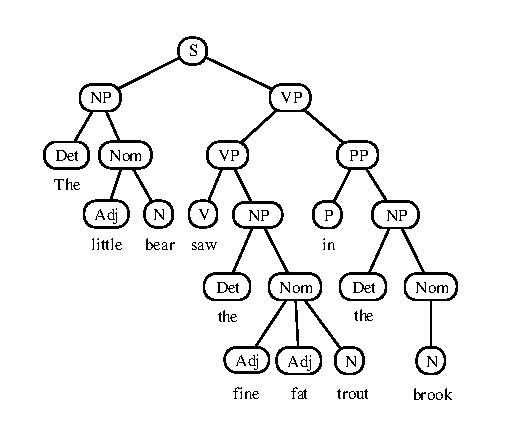
\includegraphics[width=.7\textwidth]{tree.pdf}}
    \vspace{-\baselineskip}
\end{figure}

В предлагаемом подходе немного другая грамматическая запись. Созданная грамматика представлена в (\ref{eq:grammar1}).
\begin{equation}
    \label{eq:grammar1}
    \left\{ 
        \begin{array}{l}
            D \rightarrow S\ |\ S\ D\ |\ S\ \ U\ D\ \\
            S \rightarrow NPG\ \ \ VBG \\
            VPG \rightarrow VP\ |\ VP\ \ VPG\ |\ VP\ \ U\ \ VPG \\
            NPG \rightarrow NP\ |\ NP\ \ NPG\ |\ NP\ \ U\ \ NPG \\
            AJPG \rightarrow AJ\ |\ AJ\ \ APG\ |\ AJ\ \ U\ \ APG \\
            AVPG \rightarrow AV\ |\ AV\ \ APG\ |\ AV\ \ U\ \ APG \\
            VP \rightarrow V APG\ |\ V\ \ PPG\ |\ V\ \ PP\ \ APG \\
            NP \rightarrow NOM\ |\ DET\ \ NOM \\
            NOM \rightarrow N\ |\ AJPG\ \ N \\
            PP \rightarrow NPG\ |\ P\ \ NPG
        \end{array}
    \right.\ ,
\end{equation}
\makebox[12.5mm]{где\hfill}$D$ -- документ,\\
\makebox[12.5mm]{}$SB$ -- синтаксическая основа предложения с его зависимостями,\\
\makebox[12.5mm]{}$U$ -- союз,\\
\makebox[12.5mm]{}$NPG$ -- группа именных фраз,\\
\makebox[12.5mm]{}$VPG$ -- группа глагольных фраз,\\
\makebox[12.5mm]{}$AJPG$ -- группа однородных прилагательных,\\
\makebox[12.5mm]{}$AVPG$ -- группа однородных наречий,\\
\makebox[12.5mm]{}$PPG$ -- группа однородных дополнений,\\
\makebox[12.5mm]{}$VP$ -- глагольная группа,\\
\makebox[12.5mm]{}$NP$ -- именная группа,\\
\makebox[12.5mm]{}$NOM$ -- номинальная группа,\\
\makebox[12.5mm]{}$P$ -- предлог,\\
\makebox[12.5mm]{}$AJ$ -- прилагательное,\\
\makebox[12.5mm]{}$AV$ -- наречие,\\
\makebox[12.5mm]{}$PP$ -- существительное с предлогом,\\
\makebox[12.5mm]{}$N$ -- существительное,\\
\makebox[12.5mm]{}$V$ -- глагол,\\
\makebox[12.5mm]{}$DET$ -- определяющее слово.

 Грамматика из формулы (\ref{eq:grammar1}) позволяет рекурсивно выделять основу предложения и последовательности глагола, существительного, прилагательного, наречия и т.д. Это все еще не идеальное решение, но попытка найти более сложные предложения в политиках безопасности. Этот подход требует использования пулов синонимов, которые соответствуют различным ключевым словам. Поэтому в грамматику включены метки пулов синонимов, привязанных к части речи. Метки пулов вручную назначены частям речи для преобразования привязок частей речи NLTK, это показано в формуле (\ref{eq:grammar2}).
\begin{equation}
    \label{eq:grammar2}
    \left\{ 
        \begin{array}{l}
            U \rightarrow NLTK\_CC \\
            DET \rightarrow NLTK\_DT \\
            AJ \rightarrow NLTK\_JJ \\
            AV \rightarrow NLTK\_RB \\
            N \rightarrow \_\_CN\_\_\ |\ \_\_FP\_A\_\_\ |\ \_\_TP\_A\_\_\ |\ NLTK\_N \\
            V \rightarrow \_\_CV\_\_\ |\ NLTK\_V
        \end{array},
    \right. 
\end{equation}
\makebox[12.5mm]{где\hfill}$NLTK\_CC$ -- соединение NLTK,\\
\makebox[12.5mm]{}$NLTK\_N$ -- все формы существительных NLTK,\\
\makebox[12.5mm]{}$NLTK\_В$ -- все формы глаголов NLTK,\\
\makebox[12.5mm]{}$NLTK\_DET$ -- определители NLTK,\\
\makebox[12.5mm]{}$NLTK\_RB$ -- все формы наречий NLTK,\\
\makebox[12.5mm]{}$\_\_FP\_A\_\_$ -- метка актора-обладателя персональных данных,\\
\makebox[12.5mm]{}$\_\_TP\_A\_\_$ -- третья сторона,\\
\makebox[12.5mm]{}$\_\_CV\_\_$ -- глагол сбора,\\
\makebox[12.5mm]{}$\_\_CN\_\_$ -- существительное сбора.

Теги, начинающиеся с подчеркивания, являются метками пулов синонимов. Синтаксический анализ выполняет библиотека NLTK. На основе предложенной грамматики, описанной (\ref{eq:grammar1}) и (\ref{eq:grammar2}) и разметки лейблами пулов было построено дерево предложения, результат на рисунке \ref{fig:tree}.

\begin{figure}[H]
    \centering
    \ffigbox[\FBwidth]
    {\caption{Дерево грамматического разбора\label{fig:tree}}}
    {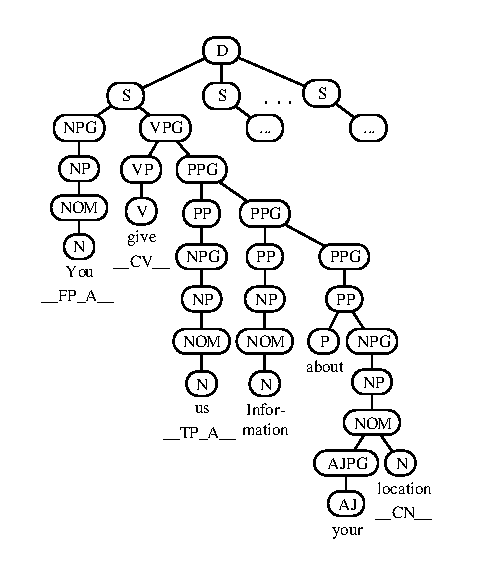
\includegraphics[width=.7\textwidth]{labeled_tree.pdf}}
    \vspace{-\baselineskip}
\end{figure}

Когда было построено дерево предложений последовательность меток ключевых слов может быть распознана. В этом случае представленная на рисунке \ref{fig:tree}, последовательность <<\_\_FP\_A\_\_>>, <<\_\_CV\_\_>>, <<\_\_CN\_\_>> хорошо видна. Такие атомарные последовательности, раскрывают значения частей предложения и могут быть объединены в список, после этого весь смысл документов будет описан этим список. Сочетание маркировки ключевых слов и синтаксического анализа дает значения ключевых слов с отношениями между этими словами, определенными в виде древовидных структур. Дерево структура данных более гибкая, чем строка предложения, деревья и особенно поддеревья показывают важные отношения между словами. Запросы к таким структурам могут дать необходимую информацию для построения логических последовательностей действующих лиц, их действий, субъектов этих действий и, наконец, обстоятельств. Предлагаемый подход определенно имеет такие недостатки, как низкая производительность, вручную определенные пулы синонимов и т.д.


В результате апробации алгоритма латентно-семантического анализа было выяснено что для кластеризации экстремально схожих между собой текстов он  подходит не лучшим образом. В связи с этими обстоятельствами было решено обратить внимание на несколько иной подход анализа текста, основанный на контекстно-свободных грамматиках, тегировании по частям речи и синонимическом поиске.

\subsection{Выводы по строгим методам текстового анализа}

Эксперименты показали, что оба рассмотренных метода имеют как преимущества, так и определенные недостатки. Хотя предложенные подходы, оказались противоречивыми, окончательные результаты заслуживают внимания. Подход с латентно-семантическим поиском оказался не слишком эффективным. Однако, подход основанный на грамматическом анализе предложений и синонимическом поиске дал определенные результаты. Хоть он и не является производительным, с его помощью возможно производить выделение логических цепочек из предложений для получения более формального описания политик безопасности нежели их текстовые варианты.

\subsection{Подход основанный на глубоком обучении}
Исходя из проведенных исследований стало понятно, что более предпочтительным вариантом решения задачи будет подход с применением моделей с глубоким обучением. Реализация подобного проекта -- комплексная задача, ее можно разделить на несколько этапов. Сначала необходимо собрать датасет, потом его разметить для обучения модели, далее обучить модель и получить результаты. Однако сбор датасета тоже является непростой задачей. Для того чтобы осуществить сбор датасета необходим инструмент для поиска и скачивания вэб-страниц из сети интернет. Затем необходимо произвести очистку данных, удалить все теги со страниц, чтобы можно было передать текст аннотаторам. Все этапы сбора датасета полагаются на базу данных. Она лишена сложного объектно-реляционного моделирования, так как в ней по сути необходимо только хранить промежуточные результаты обработки текстовых файлов.

\newpage
\section{Проектирование инструментария}

\subsection{Техническое задание <<Инструментарий для сбора датасета>>}

\subsubsection{Основные положения технического задания}

\subsubsection{Скрейпер вэб-страниц}
Скачивание веб-страниц будет производиться инструментом написанным на языке Python, с помощью библиотек можно скачивать страницы анализировать данные с них, переходить по гиперссылкам и много другое. Такой инструмент позволит просматривать и сохранять содержимое страниц в автоматическом режиме без вмешательства пользователя. Таким образом в автоматическом режиме можно сохранить и проанализировать огромное количество текстовой информации.

\subsubsection{Очистка скачанных страниц политик}
Для очистки страниц от кода разметки планируется использовать библиотеку <<html sanitizer>>. Очистка кода необходима для того, чтобы аннотаторы могли максимально сфокусироваться на анализе текста, таким образом получая чистый текст они не будут отвлекаться на не имеющие значения в контексте задачи фрагменты.

\subsubsection{Инструмент разметки датасета}
Инструмент разметки датасета планировалось реализовать с помощью веб-технологий. Серверная часть будет полагаться на приложение, написанное на PHP, которое будет регулировать порядок выдачи текста на аннотирование. Процесс разметки высокодинамичен, поэтому невозможно избежать написания качественной клиентской части приложения на языке javascript. Это позволит сделать работу аннотаторов максимально производительной, в <<одну сессию>>, так как страница не будет перезагружаться, однако все изменения, которые будут вносится, сохранятся.

\subsubsection{Фреймворк глубокого обучения}
Для создания и тренировки модели анализа текста планируется использовать фреймворк машинного обучения <<Keras>>. Он позволяет быстро создавать классификаторы с самыми разными конфигурациями и любых типов.

После того как классификатор будет сконфигурирован останется лишь обучить его на датасете, полученном ранее.

Обученный классификатор будет в состоянии определять различные характеристики политики безопасности и аспекты обращения с данными, что позволит в автоматическом режиме формировать краткие отчеты о безопасности предоставляемого соглашения.

\subsection{Методика сбора}
Планируя решение появившейся задачи важно уделить внимание источникам дынных для сбора, потому что без них невозможно будет продолжать работу. Это важно еще и потому что необходимо будет адоптировать инструмент сбора данных под конкретные веб-ресурсы, так как на каждом из них реализована собственная html-разметка.

Исходя из ориентированности дата сета на умные устройства, логичным выглядит обращение к крупным торговым площадкам, так как они занимаются дистрибьюцией подобных устройств. На сайтах торговых площадок можно осуществлять поиск продукции и получать данные о ней в том числе и производителя продукции. Типовая разметка веб-страниц располагает для получения такой информации, так как существует лишь несколько вариантов наполнения страницы продукции.

Торговые площадки не предоставляют ссылки на официальные сайты производителей. Поэтому необходимо организовать поиск официальных сайтов производителей. Поисковые движки предоставляют API для поиска, однако некоторые из них являются платными, другие выдают совершенно неприемлемые результаты. С другой использование поисковых движков, предназначенных для реальных пользователей, дает наилучшие результаты из возможных, скорее всего это связано с клиентоориентированностью, то есть получая запрос близкий к наименованию бренда с большей вероятностью будет выдана официальная страница производителя в Интернете.

Далее важной задачей является определение какая из ссылок в результате запроса наиболее четко соответствует искомому производителю. Получение официальных веб-сайтов производителей задача на первый взгляд сложная, однако результаты ручной проверки показали, что лучшим вариантом является поисковый запрос с названием производителя <<как есть>>. В таком случае вебсайт производителя оказывается на первой странице результата поискового запроса, а если не оказывается, значит у этой компании его с очень большой вероятностью нет. 

Получив ссылки предполагаемых официальных сайтов, мы получаем доступ к страницам, на которые они ведут. Поиск политики безопасности на уже обнаруженном сайте производителя является тривиальной задачей. Сейчас на абсолютном большинстве сайтов в футере имеется ссылка, названная как “Privacy” или “Privacy Policy”. Футер доступен на любой странице сайта и является частью глобальной навигационной системы сайта, в него вынесена информация, которая пригождается не так часто как, например, информация из верхних баров и меню, однако тем не менее эта информация важна, и помимо ссылок на политику безопасности зачастую содержит контактные данные и прочую организационную информацию.

Таким образом можно получить ссылки на политики безопасности производителей умной продукции. Далее необходимо произвести обработку скачанных политик безопасности.

\subsection{Методика очистки}

Очистка политик безопасности является комплексной задачей. Получив политику безопасности, необходимо вырезать все теги, которые несут в себе динамику, то есть все элементы управления. Такие элементы как всплывающие модальные диалоговые окна тоже не могут содержать текст политики безопасности. Изображения, помещенные на странице, так же не относятся к политике безопасности. Таким образом получается, что большое количество тегов необходимо агрессивно удалять еще до начала анализа страницы, так как они точно не содержат полезной информации.

Далее необходимо применить обработку, которая включала бы в себя преобразование разметки: недопустимые теги должны быть развернуты, определенные комбинации вложенных тегов должны быть заменены на более тривиальные. Также необходимо очистить теги от атрибутов, так как в них не содержится полезной информации или чего-либо способного положительно сказаться на структуре очищенного документа. Затем по всему дереву DOM осуществляется рекурсивный обход с целью слияния тегов, где это возможно, или оборачивания сырых текстов. В ходе данного этапа также производится нормализация пунктуации и настройки отступов текстов, чтобы привести их к читабельному виду. 

После указанных двух этапов очистки, следует заключительный, на котором из тегов извлекается текст, то есть параграфы, представленные в виде одной длинной строки. Это делается, потому что расставленные определенным образом переводы на новую строку могут по тем или иным причинам не подходить, и это будет более гибким решением, потому что где требуется можно применить лайн-врапинг.

\subsection{Методика разметки}
Текст\dots

\subsection{Потенциальные проблемы}
Еще до решения задачи были выделены потенциальные проблемы, способные замедлить процесс разработки и сбора дата сета. Потенциально возможные проблемы при реализации приложений по добного типа следующие:
\begin{enumerate}
    \item блокировка из-за подозрительных заголовков браузера,
    \item блокировка из-за слишком частого обращения с запросами,
    \item как следствие 2-х предыдущих пунктов требование подтвердить, что это не попытка автоматического доступа (ввод капчи).
    \item Невидимые элементы разметки,
    \item динамически формируемые страницы торговых площадок и политик безопасности,
    \item промахи при сборе данных из-за частично некорректных результатов поиска на торговых площадках и в поисковых движках.
\end{enumerate}

Проблемы 1, 2, 3 решаются использованием разных заголовков браузера попеременно. Также отправка запросов ограничена по частоте от 2 до 6 секунд, ограничение выбирается случайным образом. Такие решения позволяют крайне редко попадать под подозрения, потому что в таком случае поведение максимально похоже на поведение реального пользователя, соответственно процент успеха при попытке получить данные с веб-страницы значительно повышается. Стоит отметить, что данные ограничения очень эффективно обходятся за счет использования прокси-серверов, которые позволяют менять ip-адреса. Еще одним важным и эффективным инструментом для является профиль браузера. Он позволяет запускать безголовый браузер с определенной историей использования будь то куки-файлы, история запросов или аутентификация на различных сервисах. Наличие такой предыстории у браузера для некоторых сайтов является доказательством, что он не автоматизирован.

Проблема 4 решается следующим образом. Попав на страницу политики безопасности, можно исполнить код на javascript, который загрузит на страницу библиотеку для работы с деревом DOM и удалит невидимые элементы разметки.

Проблема 5 решается использованием безголового браузера, который полнофункционален с точки зрения воспроизведения контента, так как поддерживает исполнение javascript кода на странице. Таким образом страница будет загружена и динамические элементы будут созданы, после чего можно будет их обработать. Однако на некоторых веб-сайтах для того, чтобы получить ту или иную информацию необходимо заполнить форму. С такими обстоятельствами сложно бороться – разметка всегда различается, но таких случаев крайне мало, поэтому исключение их из рассмотрения будет оправданным.

Проблема 6 может отчасти решиться конкретизацией поискового запроса путем прибавления к названию производителя ключевых слов и продукции, которая им производится. Хотя этот вариант и показал гораздо более качественные результаты нежели чем поиск производителя <<как есть>>, иногда все же попадается шум.

\subsection{Приложение вэб-скрейпер}

\subsubsection{Первичная декомпозиция и планирование}

Начальным этапом решения задачи является первичная декомпозиция, в ее результате выделяются подзадачи различной важности, которые должны быть решены для доведения цикла разработки до конца. В данном случае можно выделить следующие подзадачи:
\begin{enumerate}
    \item определение источника информации о различной IoT-продукции,
    \item отправка поискового запроса,
    \item получение результатов запроса (список IoT-продуктов),
    \item определение производителей IoT-продукции,
    \item поиск официальных сайтов производителей в сети интернет,
    \item поиск раздела <<политика безопасности>> на сайтах производителей,
    \item скачивание политик безопасности,
    \item очистка скачанных веб-документов от лишних элементов разметки,
    \item слияние тегов и оборачивание сырого текста,
    \item нормализация пунктуации и отступов,
    \item извлечение текста из тегов.
\end{enumerate}

Получение списка производителей возможно на электронных торговых площадках, типовая разметка веб-страниц располагает для получения такой информации, так как существует лишь несколько вариантов наполнения страницы продукции.

Получение официальных веб-сайтов производителей задача на первый взгляд сложная, однако результаты ручной проверки показали, что лучшим вариантом является поисковый запрос с названием производителя <<как есть>>. В таком случае веб-сайт производителя оказывается на первой строчке результата поискового запроса, а если не оказывается, значит у этой компании его с очень большой вероятностью нет.

\subsubsection{Структура приложения вэб-скрейпера}
Исходя из результатов декомпозиции, эффективным подходом выглядит представление приложения в виде последовательно выполняющихся подпрограмм так, что входом модуля является результат работы предыдуще\-го модуля, то есть в виде конвейера. Схема организации приложения предста\-влена на рисунке \ref{fig:pipeline}.

\begin{figure}[H]
    \centering
    \ffigbox[\FBwidth]
    {\caption{Схема организации приложения\label{fig:pipeline}}}
    {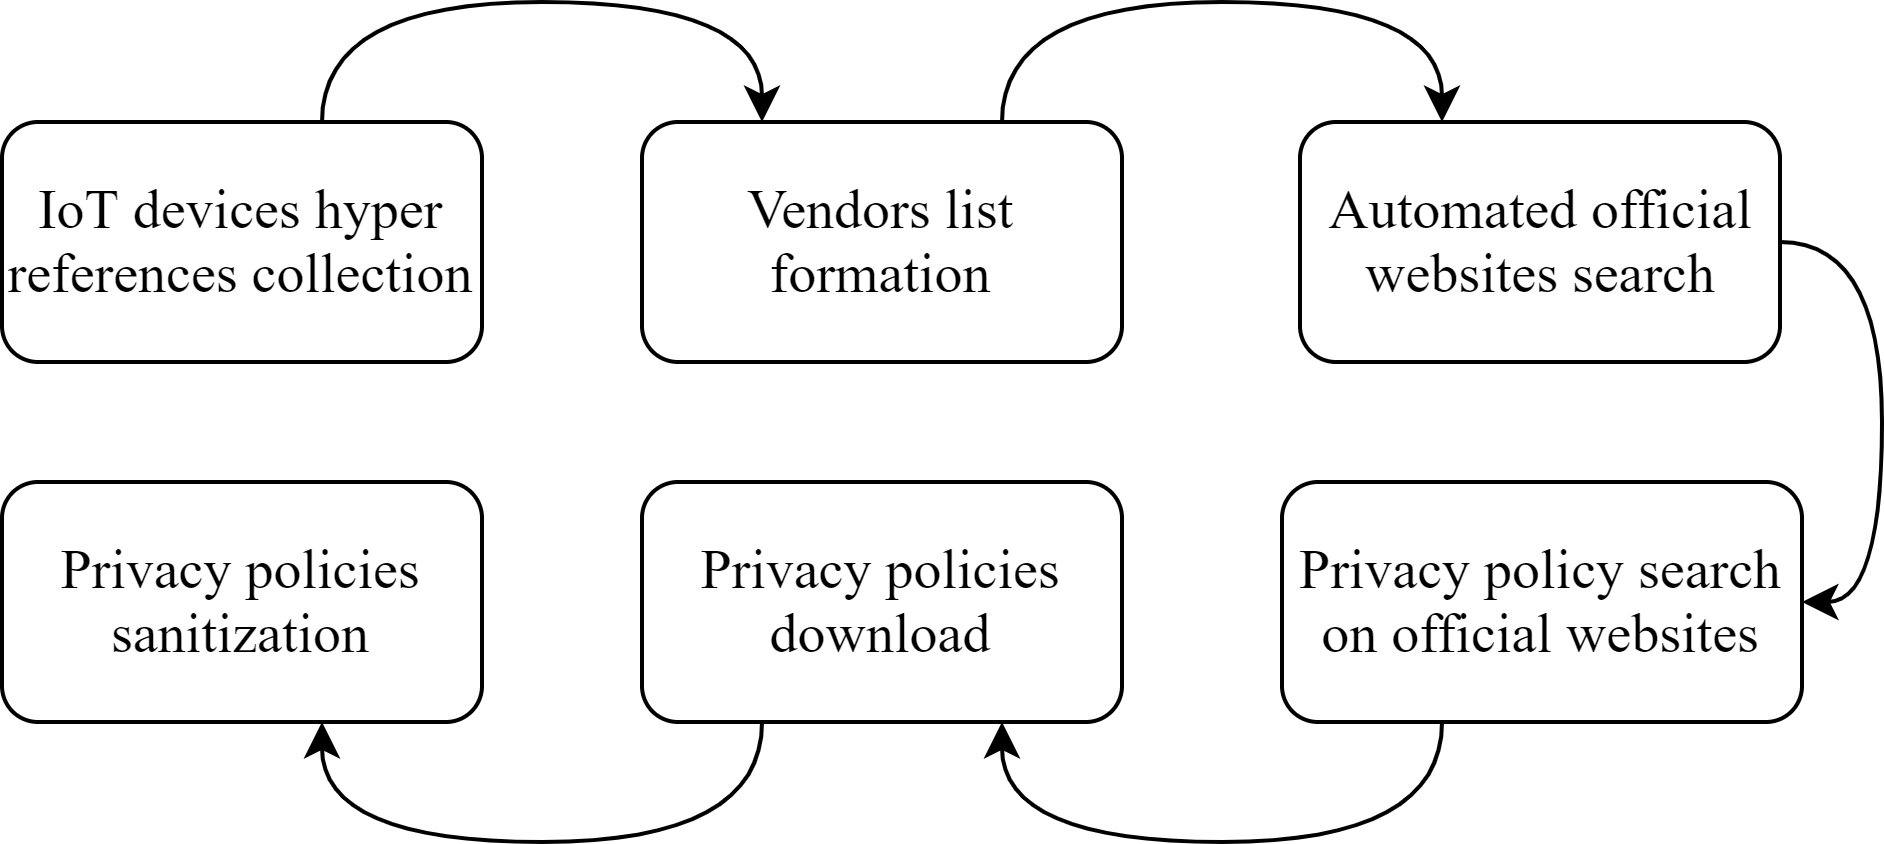
\includegraphics[width=\textwidth]{pics_pipeline.png}}
    \vspace{-\baselineskip}
\end{figure}

Далее была разработана композиционная модель приложения, на ней присутствуют все необходимые для решения задач модули. Схема представлена на рисунке \ref{fig:composition}.

\begin{figure}[H]
    \centering
    \ffigbox[\FBwidth]
    {\caption{Композиционная модель приложения\label{fig:composition}}}
    {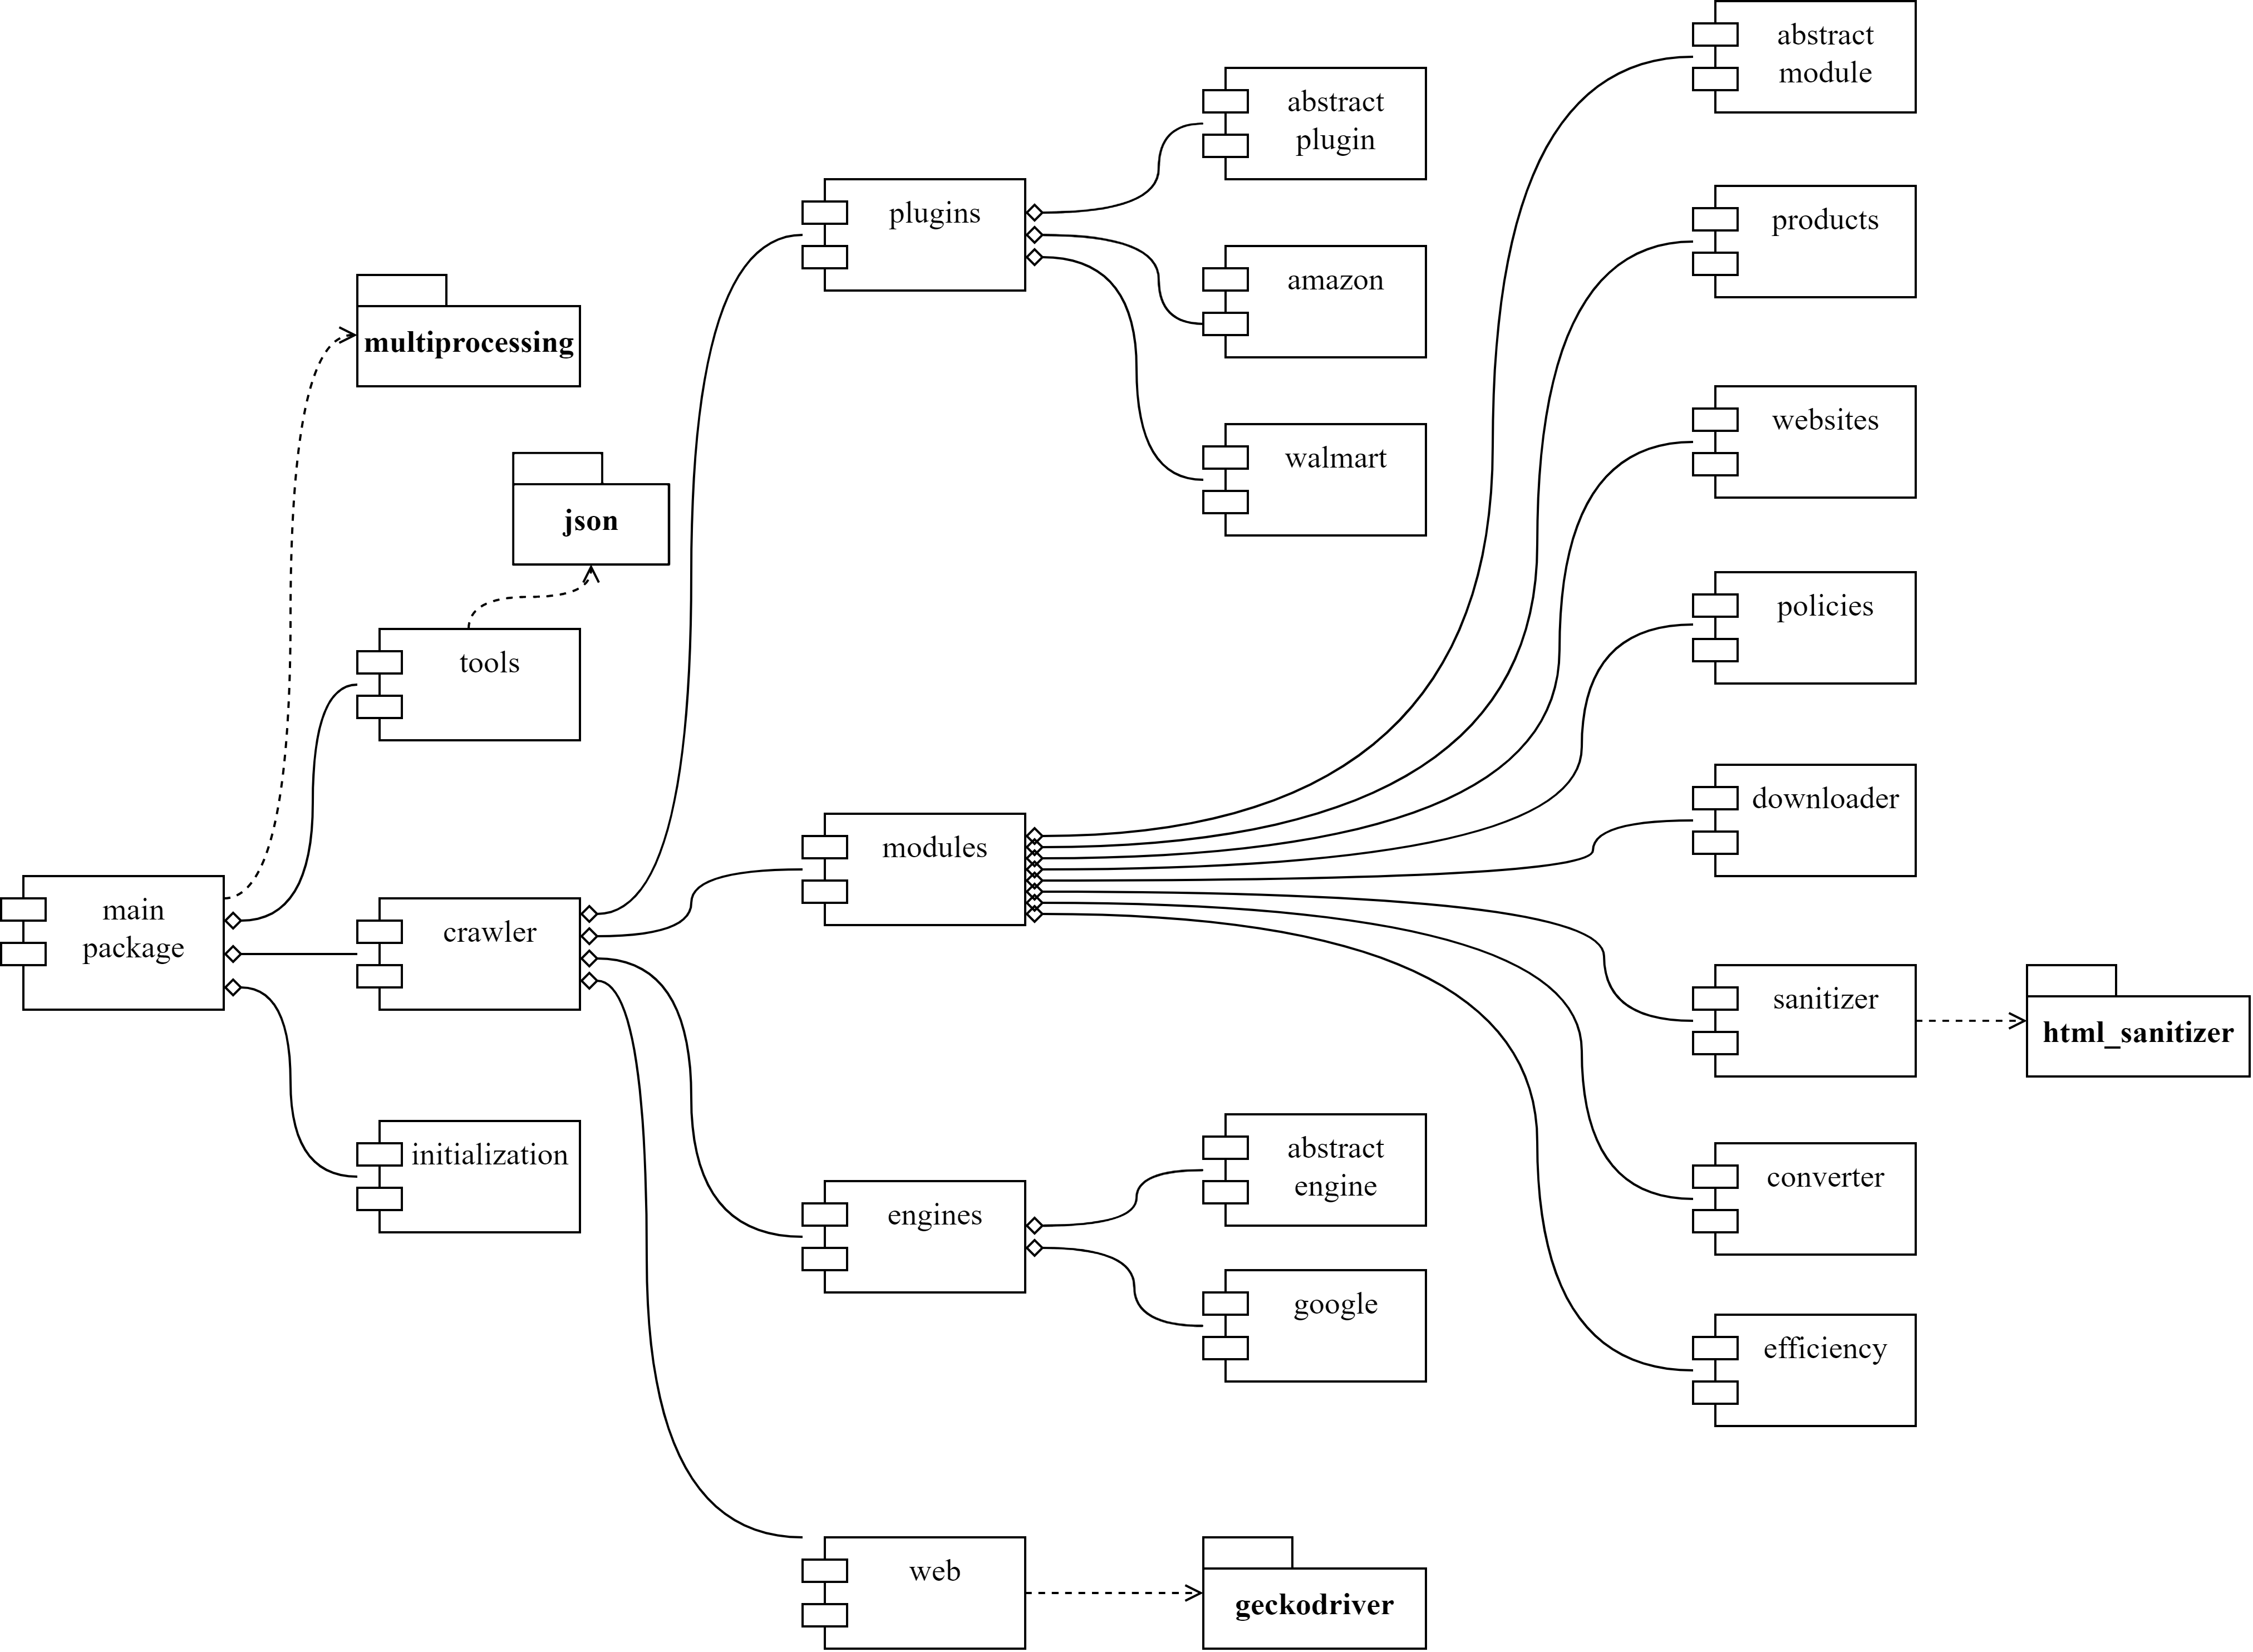
\includegraphics[width=\textwidth]{pics_modules.png}}
    \vspace{-\baselineskip}
\end{figure}

\subsubsection{Средства разработки вэб-скрейпера}
Для реализации приложения были выбраны следующие средства:
\begin{enumerate}
    \item python 3.9,
    \item <<безголовый>> браузер Firefox,
    \item драйвер для управления <<безголовым>> браузером <<geckodriver>>,
    \item библиотека html-sanitizer для очистки скачанных веб-документов. 
\end{enumerate}

Выбор <<безголового>> браузера обусловлен потребностью в отрисовке страниц, так как на некоторых веб-страницах разметка генерируется с помощью javascript. Это делает невозможным использование простого скачивания, не обходима страница именно с исполненными скриптами, в противном случае будет невозможно получить требуемую информацию. В то же время браузер лишен графического интерфейса, чем снижается потребление вычислитель ных ресурсов. 

Таким образом приложение построено на 4 основных абстракциях.

\begin{enumerate}
    \item Концепция модуля – одна из основополагающих, так как модулем в данном случае выступает любая подпрограмма, участвующая в сборе данных, принимающая входные данные в виде json-файла, и на выходе дающая так же json-файл чтобы следующий в очереди модуль мог отработать. Модули могут быть написаны с нуля, а могут расширять возможности уже существующих посредством механизма наследования. Таким образом можно не переписывая существующий код, а только добавляя новый изменять поведение программы и адаптировать ее под разные задачи сбора данных.
    \item Концепция конвейера – этот элемент поочередно вызывает модули и передает данные из одного модуля в другой. В результате отработки всех модулей поэтапно решается поставленная задача, то есть сбор данных из интернет-источников. Конвейер может быть сконфигурирован, в него могут быть помещены любые модули, реализующие соответствующий интерфейс. Также может быть сконфигурирована последовательность запуска модулей сбора данных.
    \item Концепция поискового движка – данная концепция порождена в связи с необходимостью сделать приложение как можно более гибким. Такой абстрактный элемент позволяет менять используемые поисковые движки, применять к результатам поиска алгоритмы для определения какие результаты удовлетворяют условиям поиска, а какие нет.
    \item Концепция плагина – плагин обеспечивает сбор данных с какой-либо конкретной торговой площадки. Данная концепция использована так же для обеспечения гибкости приложения – для устранения привязки к набору конкретных торговых площадок. Использую механизм наследования можно переопределить поведение плагина для работы с любой другой торговой площадкой. 
\end{enumerate}

На рисунке 2 модуль <<main>> отвечает за запуск программы, развертывание основных ее частей. Там же происходит инициализация пула процессов для мультипроцессинга затратных задач таких как, например, взаимодействие с <<безголовым>> браузером. Он так же отвечает за последовательное исполнение подпрограмм элементов конвейера. Он осуществляет прием выходных и передачу входных данных модулей.

Модуль <<initialization>> производит проверку файловой системы и создает необходимые директории в папке ресурсов.

Модуль <<tools>> содержит вспомогательные функции, в частности для ввода и вывода данных в формате json. 

Модуль <<crawler>> отвечает за получение данных с веб-страниц, в нем агрегированы все инструменты для сбора и очистки данных. 

Модуль <<plugins>> включает в себя набор плагинов, каждый из которых адаптирован для получения требуемой информации с определенного шаблона веб-страничной разметки. Некоторое поведение инкапсулировано в абстрактном плагине для увеличения <<reusability>> кода. Получая адрес на вход, данный плагин производит скачивание страницы и с помощью набора шаблонов пытается извлечь информацию. Данный модуль записывает полученную с помощью плагинов информацию в json-файл для большей прозрачности и возможности сохранения результатов между запусками приложения, например, для пропуска данного этапа и использования его сохраненных результатов работы. 

Данные полученные с помощью модулей <<products>>, <<websites>>, <<policies>>, <<downloader>>, <<sanitizer>>, <<converter>> и <<efficiency>> записывается в json-файлы для большей прозрачности и возможности сохранения результатов между запусками приложения, например, при пропуске какого-либо из этапов и использования его сохраненных результатов работы. Модуль <<products>> получение производителей IoT-продуктов. Модуль <<websites>> получение официальных сайтов производителей. Модуль <<policies>> получение веб-ссылок на политики безопасности. Модуль <<downloader>> отвечает за скачивание страниц и их сохранение в отведенную для этого директорию. Модуль <<sanitizer>> отвечает за очистку скачанных веб-страниц от не нужных тегов и ссылок. Модуль <<converter>> производит перевод политик безопасности из веб-страничного вида в текстовое представление. Модуль <<efficiency>> производит расчет статистики по дата сету.

Модуль <<web>> отвечает за взаимодействие с вебсайтами будь то торговые площадки или сайты производителей IoT-продуктов. В нем используется geckodriver для управления <<безголовым>> браузером. 

Модуль <<proxy>> содержит инструменты для скачивания и автоматического применения бесплатных прокси-серверов. Однако ввиду ненадежности бесплатных, есть так же возможность задать список выделенных прокси-серверов. 

Для обеспечения наиболее гибкой настройки как можно больше настроек выведено в отдельный конфигурационный файл. В нем задаются:

\begin{enumerate}
    \item параметры для библиотеки html-sanitizer, в частности набор допустимых тегов и допустимых атрибутов;
    \item параметры безголового браузера, в том числе количество повторных попыток при сбоях, появлении каптчи и так далее, набор юзерагентов для перебора, флаги использования кэширования, флаг запуска браузера в режиме без графического интерфейса, флаг использования прокси, пути для логов, а также путь до профиля браузера;
    \item список директорий и файлов, в которые происходит сохранение результатов сбора данных;
    \item количество процессов для одновременного сбора данных на многоядерных конфигурациях.
\end{enumerate}

Для настройки работы заменяемых элементов таких как поисковые движки плагины и модули, предусмотрены отдельные файлы, в которых создаются те или иные конфигурируемые объекты.

Учитывая конвейерную организацию и передачу результатов из модуля в модуль посредством json-файлов, структура дата сета следующая: каждый модуль имеет свой json-файл для записи результатов. По сути результаты – это массив из python-словарей, каждый словарь является своего рода кортежем, эти кортежи обладают избыточностью данных, однако, таким образом достигается максимальная простота формализации данных. Каждый элемент – IoT устройство, обладающее набором информационных полей: идентификатор; ссылка на страницу на торговой площадке; наименование производителя; ключевое слово, по которому было найдено устройство; ссылка на сайт производителя; ссылка на политику безопасности; путь к сохраненной оригинальной страницы политики безопасности; путь к очищенной политике безопасности; путь к текстовой версии политики безопасности; хэш, сгенерированный по тексту политики; блок статистики по структурным элементам, таким как нумерованные и ненумерованные списки, элементы списков, таблицы, параграфы, длина политики в символах. Пример такой разметки можно увидеть на рисунке \ref{fig:tuple}.

\begin{figure}[H]
    \centering
    \ffigbox[\FBwidth]
    {\caption{Пример кортежа дата сета\label{fig:tuple}}}
    {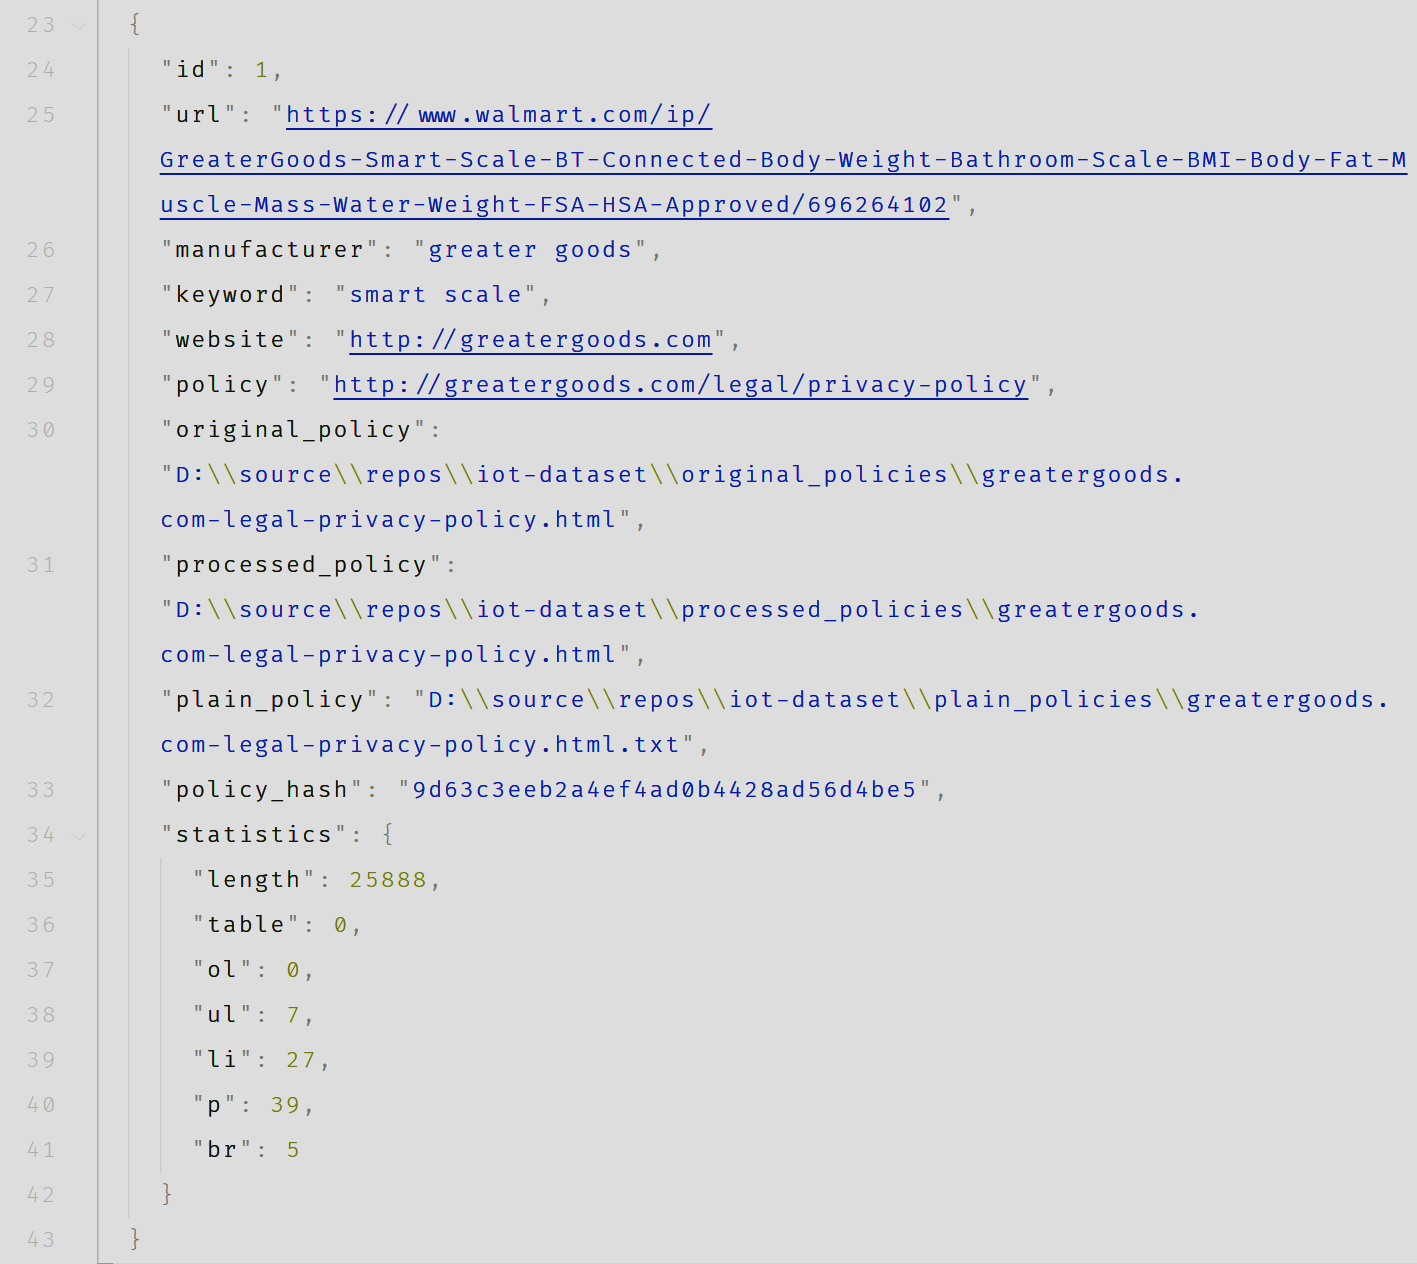
\includegraphics[width=\textwidth]{tuple.png}}
    \vspace{-\baselineskip}
\end{figure}

В веб-краулере также предусмотрена возможность явного указания адресов для скачивания политик безопасности, для чего предусмотрен отдельный json-файл, содержащий элементы со схожей структурой. В нем можно указывать любые из полей – они будут заполнены соответствующе, а незаполненные поля останутся равными <<null>>. Явно заданные для скачивания политики считываются непосредственно на этапе скачивания, таким образом данные о названии производителя и другие данные которые участвуют в более ранних стадиях сбора несут сугубо справочный характер. Статистические показатели политик безопасности рассчитываются на последнем этапе работы приложения, что означает их перезапись после каждого запуска, при условии, что модуль расчета статистики активен.

\subsection{Инструмент разметки датасета}
Инструмент разметки датасета планировалось реализовать с помощью веб-технологий. Серверная часть будет полагаться на приложение, написанное на PHP, которое будет регулировать порядок выдачи текста на аннотирование. Процесс разметки высокодинамичен, поэтому невозможно избежать написания качественной клиентской части приложения на языке javascript. Это позволит сделать работу аннотаторов максимально производительной, в <<одну сессию>>, так как страница не будет перезагружаться, однако все изменения, которые будут вносится, сохранятся.

\subsubsection{Объектное моделирование приложения}

Объектная модель инструмента представлена на рисунке \ref{fig:object}.

\begin{figure}[H]
    \centering
    \ffigbox[\FBwidth]
    {\caption{Объектная модель\label{fig:object}}}
    {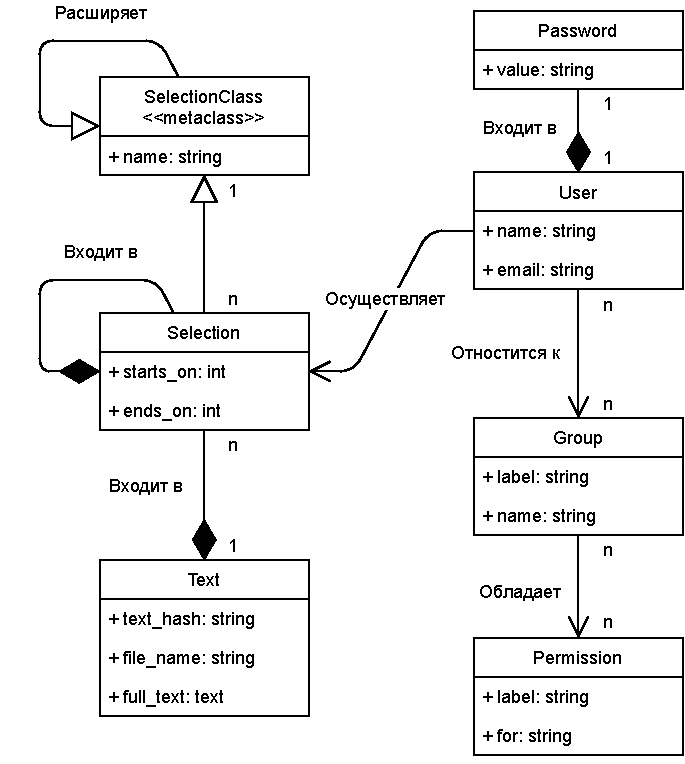
\includegraphics[width=\textwidth]{models_object.pdf}}
    \vspace{-\baselineskip}
\end{figure}

\subsubsection{Реляционная модель приложения}

Реляционная модель инструмента представлена на рисунке \ref{fig:relational}.

\begin{figure}[H]
    \centering
    \ffigbox[\FBwidth]
    {\caption{Реляционная модель\label{fig:relational}}}
    {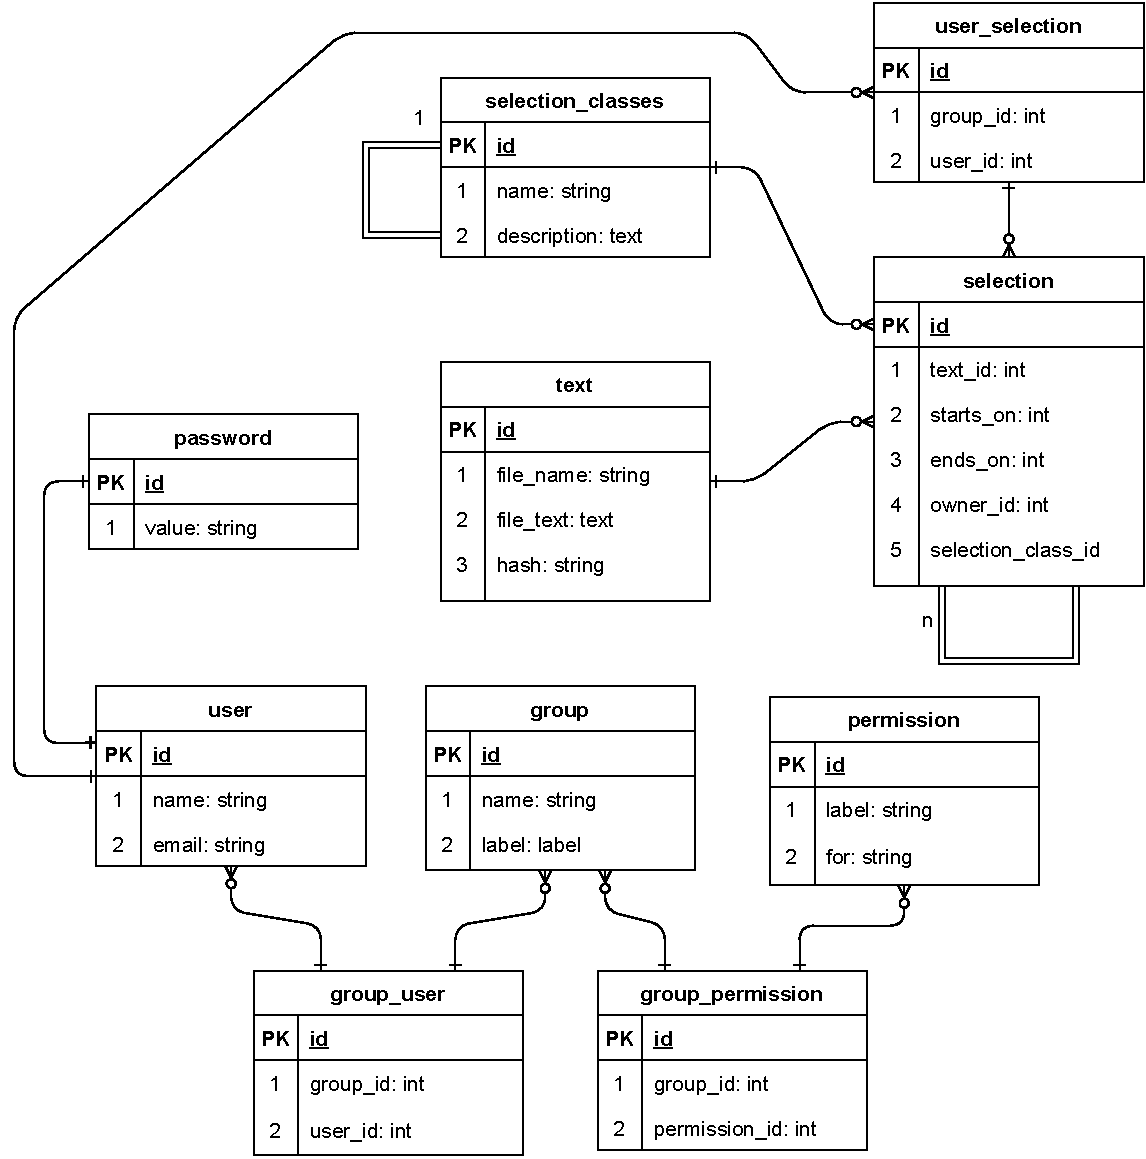
\includegraphics[width=\textwidth]{models_relational.pdf}}
    \vspace{-\baselineskip}
\end{figure}

\subsubsection{Проектирование пользовательского интерфейса}

Презентационный прототип интерфейса инструмента представлен на рисунке \ref{fig:proto}.

\begin{figure}[H]
    \centering
    \ffigbox[\FBwidth]
    {\caption{Презентационный прототип интерфейса\label{fig:proto}}}
    {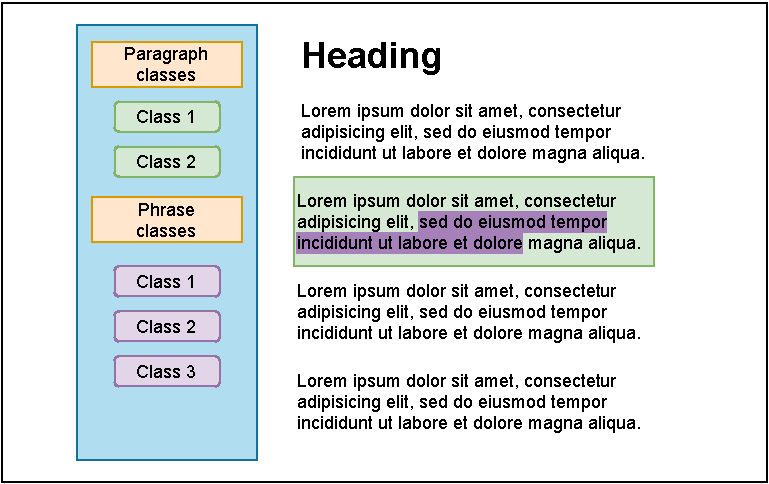
\includegraphics[width=\textwidth]{models_proto.pdf}}
    \vspace{-\baselineskip}
\end{figure}

\subsubsection{Средства разработки инструмента разметки}

\newpage
\section{Технические детали реализации инструментария}

\subsection{Полученные в результате реализации исходные коды}
В соответствии с результатами декомпозиции, выбора средств и проектирования приложение было реализовано. Характеристики полученных классов и функций приведены далее, в таблицах ?-?. Исходные коды представлены в приложениях \hyperref[sec:appendix2]{Б} и \hyperref[sec:appendix3]{В}.

\subsection{Полученный в результате сбора данных дата сет}
Поиск осуществлялся на торговых площадках amazon и walmart, брались результаты поискового запроса по первым 30-ти страницам, по категориям <<smart scale>>, <<smart watch>>, <<smart bracelet>>, <<smart lock>>, <<smart bulb>>, <<smart navigation system>>, <<smart alarm clock>>, <<smart thermostat>>, <<smart plug>>, <<smart light switch>>, <<smart tv>>, <<smart speaker>>, <<smart thermometer>>, <<smart air conditioner>>, <<smart video doorbell>>, <<robot vacuum cleaner>>, <<smart air pu\-ri\-fi\-er>>, <<gps tracking device>>, <<tracking sensor>>, <<tracking device>>, <<indoor came\-ra>>, <<outdoor camera>>, <<voice controller>>. Всего производителей было найдено приблизительно 160. Стоит отметить, что результат является приемлемым, так как многие производители на данной торговой площадке не имеют вы деленного вебсайта, а пользуются услугами amazon, то есть на таких страницах действует политика безопасности amazon, а не производителя. Также стоит отметить, что у некоторых продуктов явно не указан производитель, что    сократило количественно результат поиска.

Всего было проанализировано 57150 моделей умной продукции, из них для 51727 (90,5\%) были определены производители. Всего уникальных производителей было найдено 6161, из них 1419 (23\%) имеют официальную веб-страницу. Проанализировав найденные веб-сайты были собраны 798 политик безопасности, разумеется, среди них имеется определенный процент промахов, если производитель имеет сходство с каким-либо другим более крупным. Из дата сета были исключены политики безопасности, длина которых в символах не превышала 1000. Это объясняется тем, что некоторые производители имеют на своем сайте страницу с политикой безопасности, но по каким-то причинам эта страница не наполнена. Примеры таких случаев приведены на рисунках \ref{fig:not_found1} и \ref{fig:not_found2}. Таким образом полноценных уникальных политик безопасности осталось 592.

\begin{figure}[H]
    \centering
    \ffigbox[\FBwidth]
    {\caption{Пример отсутствующей политики\label{fig:not_found1}}}
    {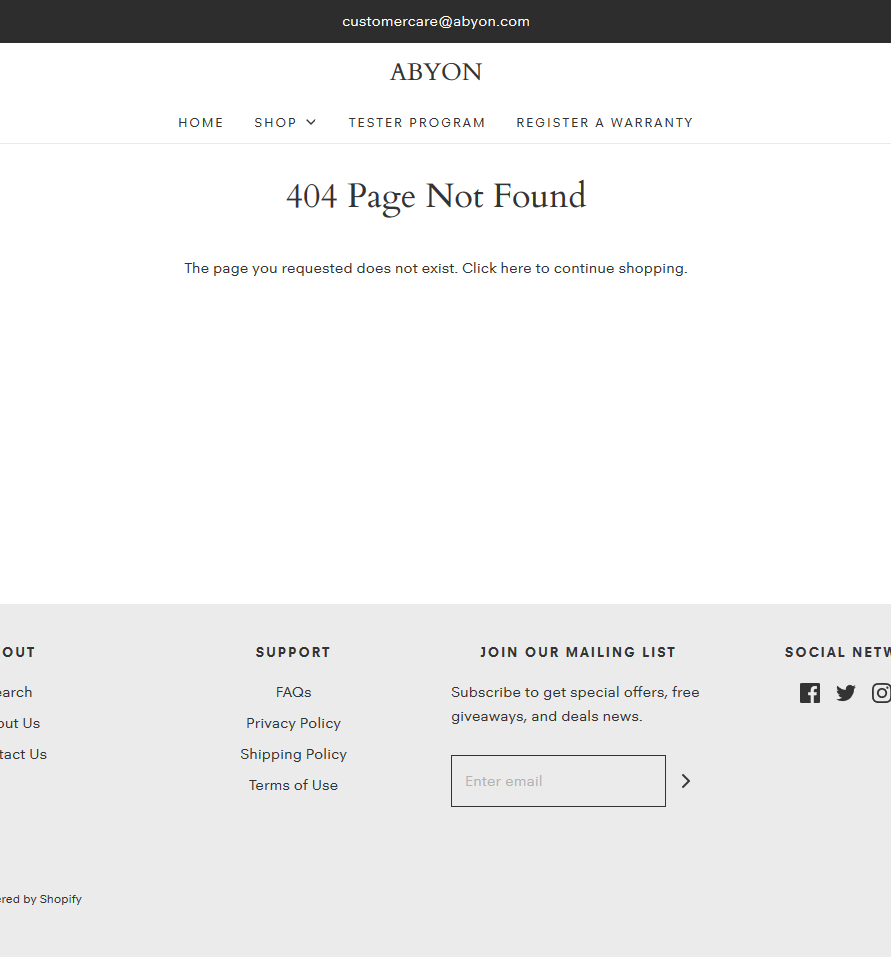
\includegraphics[width=\textwidth]{not_found1.png}}
    \vspace{-\baselineskip}
\end{figure}

\begin{figure}[H]
    \centering
    \ffigbox[\FBwidth]
    {\caption{Пример отсутствующей политики\label{fig:not_found2}}}
    {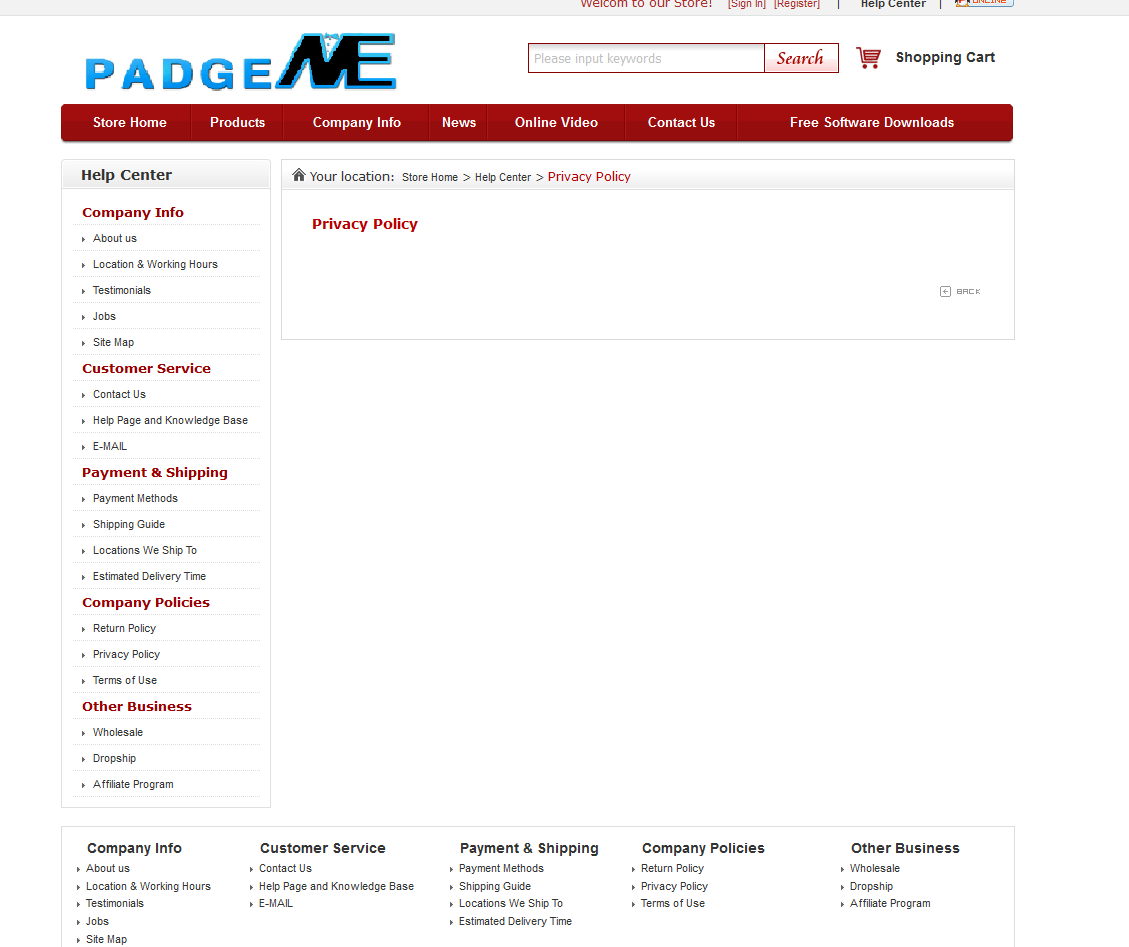
\includegraphics[width=\textwidth]{not_found2.png}}
    \vspace{-\baselineskip}
\end{figure}

Некоторые из производителей, которые не имеют собственного веб-сайта и политика безопасности которых не была найдена, пользуются услугами хостинга интернет-магазина непосредственно на amazon. В таком случае, будучи частью интернет-магазина на них распространяется политика безопасности площадки, на которой они размещают свои предложения, причем политики могут различаться для разных стран. Случаи с использованием отдельных политик безопасности под различные типы устройств не были зафиксированы, хотя такие случаи и существуют, проще прибегнуть к явному заданию адресов политик, нежели чем к попытке автоматизировать процесс сбора, так как остаются непрозрачными способы выявления подобных ситуаций.

На рисунках \ref{fig:paragraph_size} и \ref{fig:policy_size} приведены статистические данные по объемам абзацев политик и самих докумнетов соответственно.

\begin{figure}[H]
    \centering
    \ffigbox[\FBwidth]
    {\caption{Распределение политик по объему параграфа\label{fig:paragraph_size}}}
    {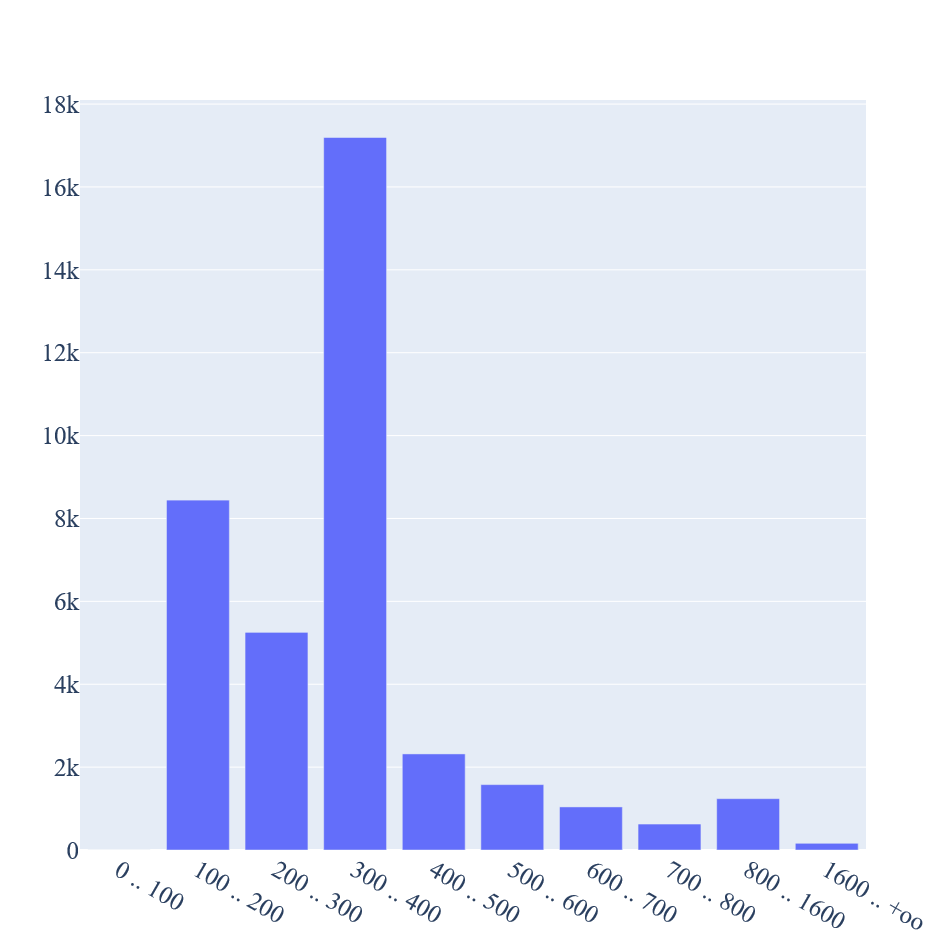
\includegraphics[width=\textwidth]{paragraph_size.png}}
    \vspace{-\baselineskip}
\end{figure}

\begin{figure}[H]
    \centering
    \ffigbox[\FBwidth]
    {\caption{Распределение политик по объему документа\label{fig:policy_size}}}
    {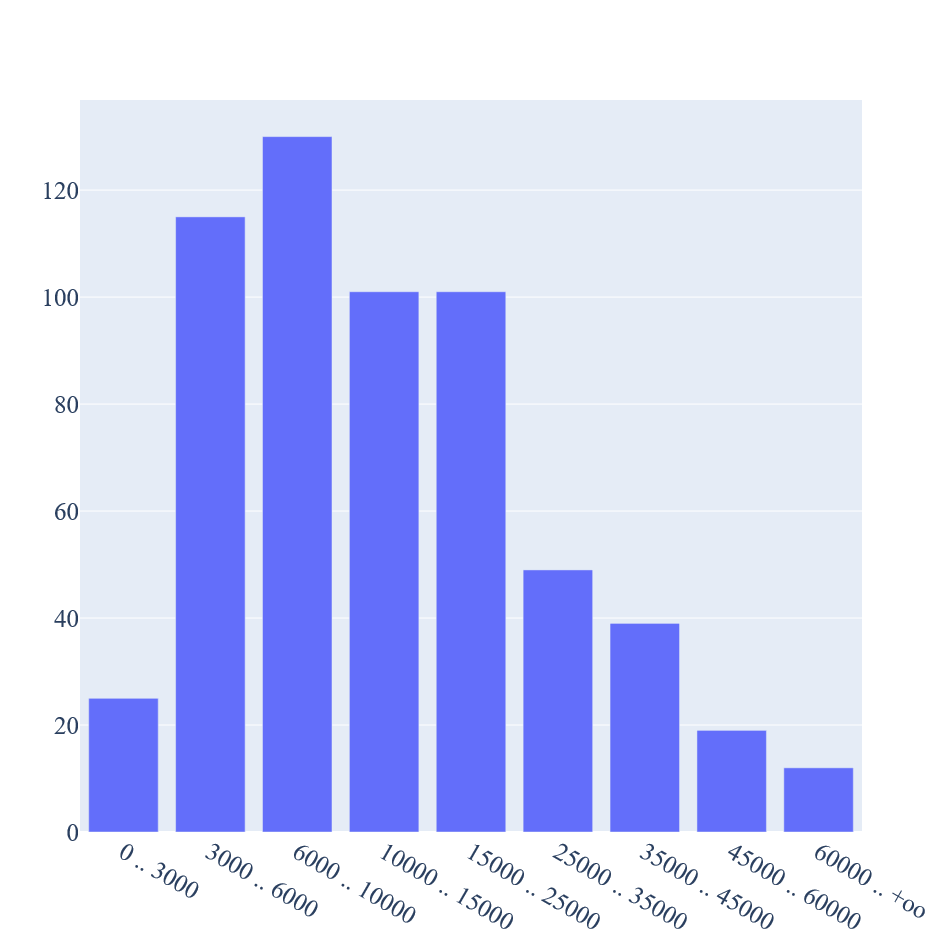
\includegraphics[width=\textwidth]{policy_size.png}}
    \vspace{-\baselineskip}
\end{figure}

Подсчет количества заголовков сложно организовать автоматизированно в связи с большим разнообразием html-разметки. На каждом сайте своя разметка, своя конвенция по нумерованию секций, заголовков, списков. На некоторых сайтах списки и заголовки нумеруются средствами html, на других нумерация проставлена вручную. Все это порождает разношерстность данных, и их обработка становится сложной с точки зрения учета всех возможных вариантов. Поэтому авторы решили прибегнуть к простому подсчету количества строк длиной меньше 100 символов и не содержащих при этом маркеров <<{list item}>>. Такой подход не даст очень точных показателей, но может дать приблизительные значения. На рисунках \ref{fig:structure_stats1} и \ref{fig:structure_stats2} приведена статистика по структурным элементам политик безопасности в двух частях. Здесь изображены детальные распределения структурных элементов для каждой из найденных политик безопасности.

\begin{figure}[H]
    \centering
    \ffigbox[\FBwidth]
    {\caption{Статистика первых 246 политик в IoT дата сете по структурным элементам\label{fig:structure_stats1}}}
    {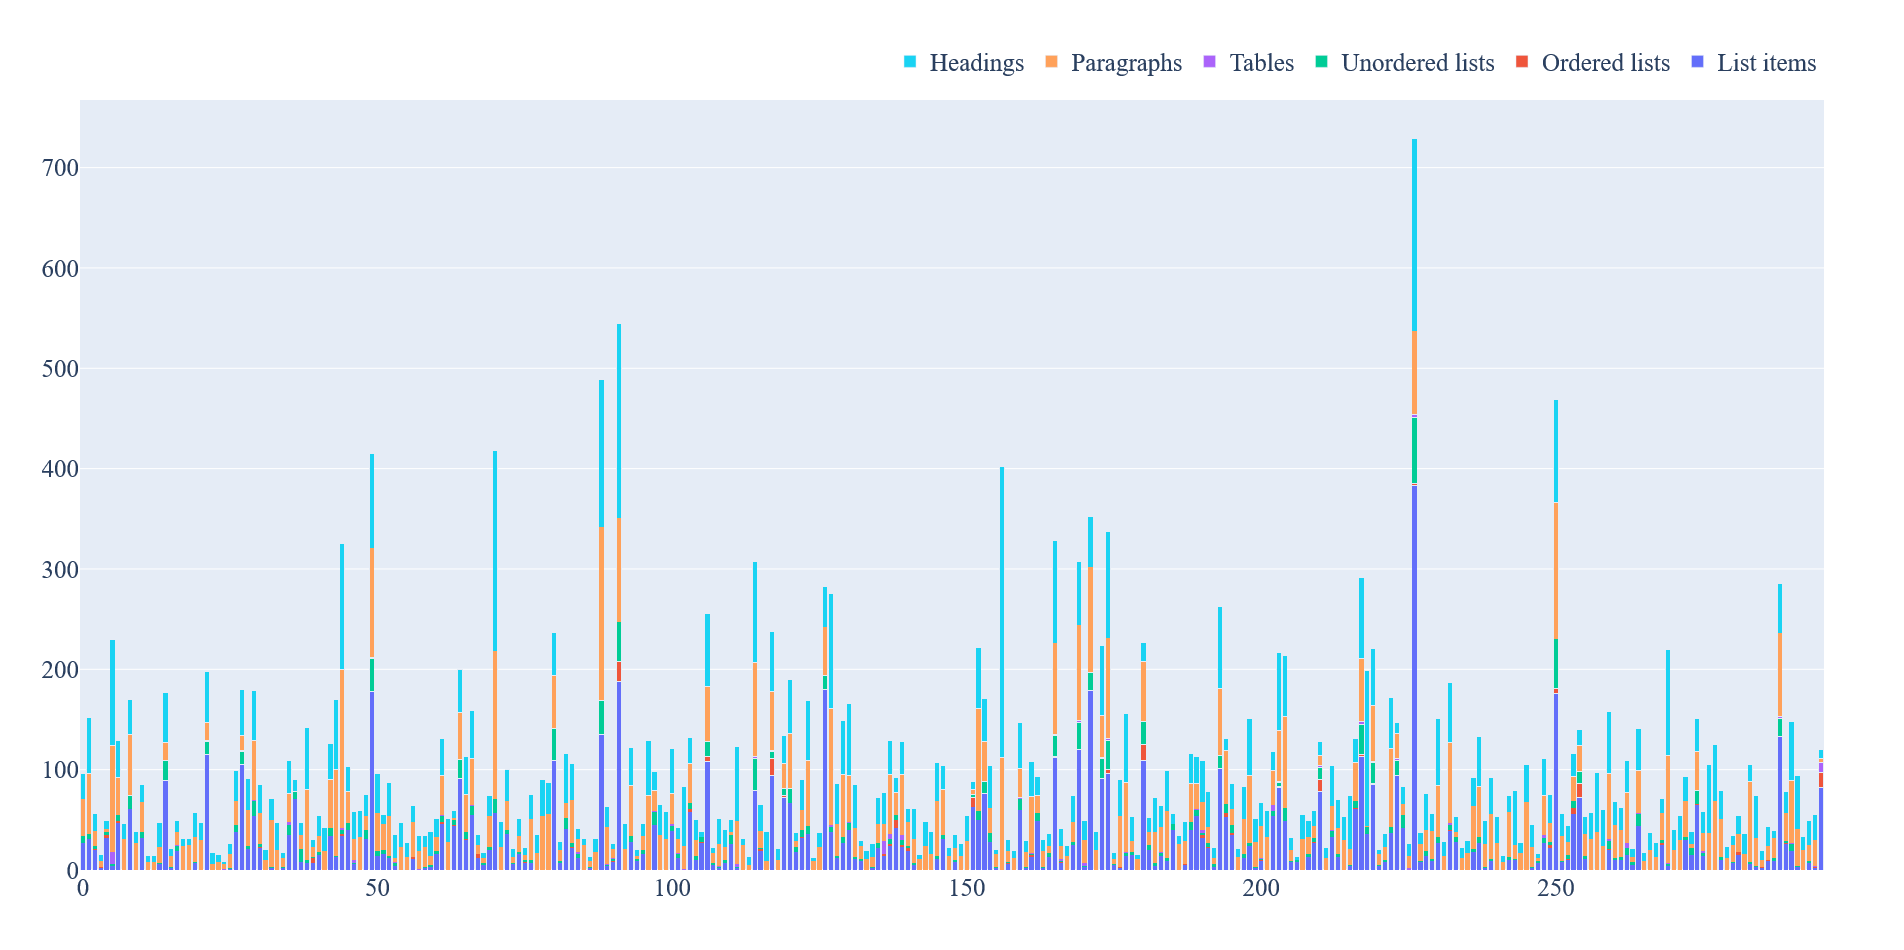
\includegraphics[width=\textwidth]{structure_stats1.png}}
    \vspace{-\baselineskip}
\end{figure}

\begin{figure}[H]
    \centering
    \ffigbox[\FBwidth]
    {\caption{Статистика последних 246 политик в IoT дата сете по структурным элементам\label{fig:structure_stats2}}}
    {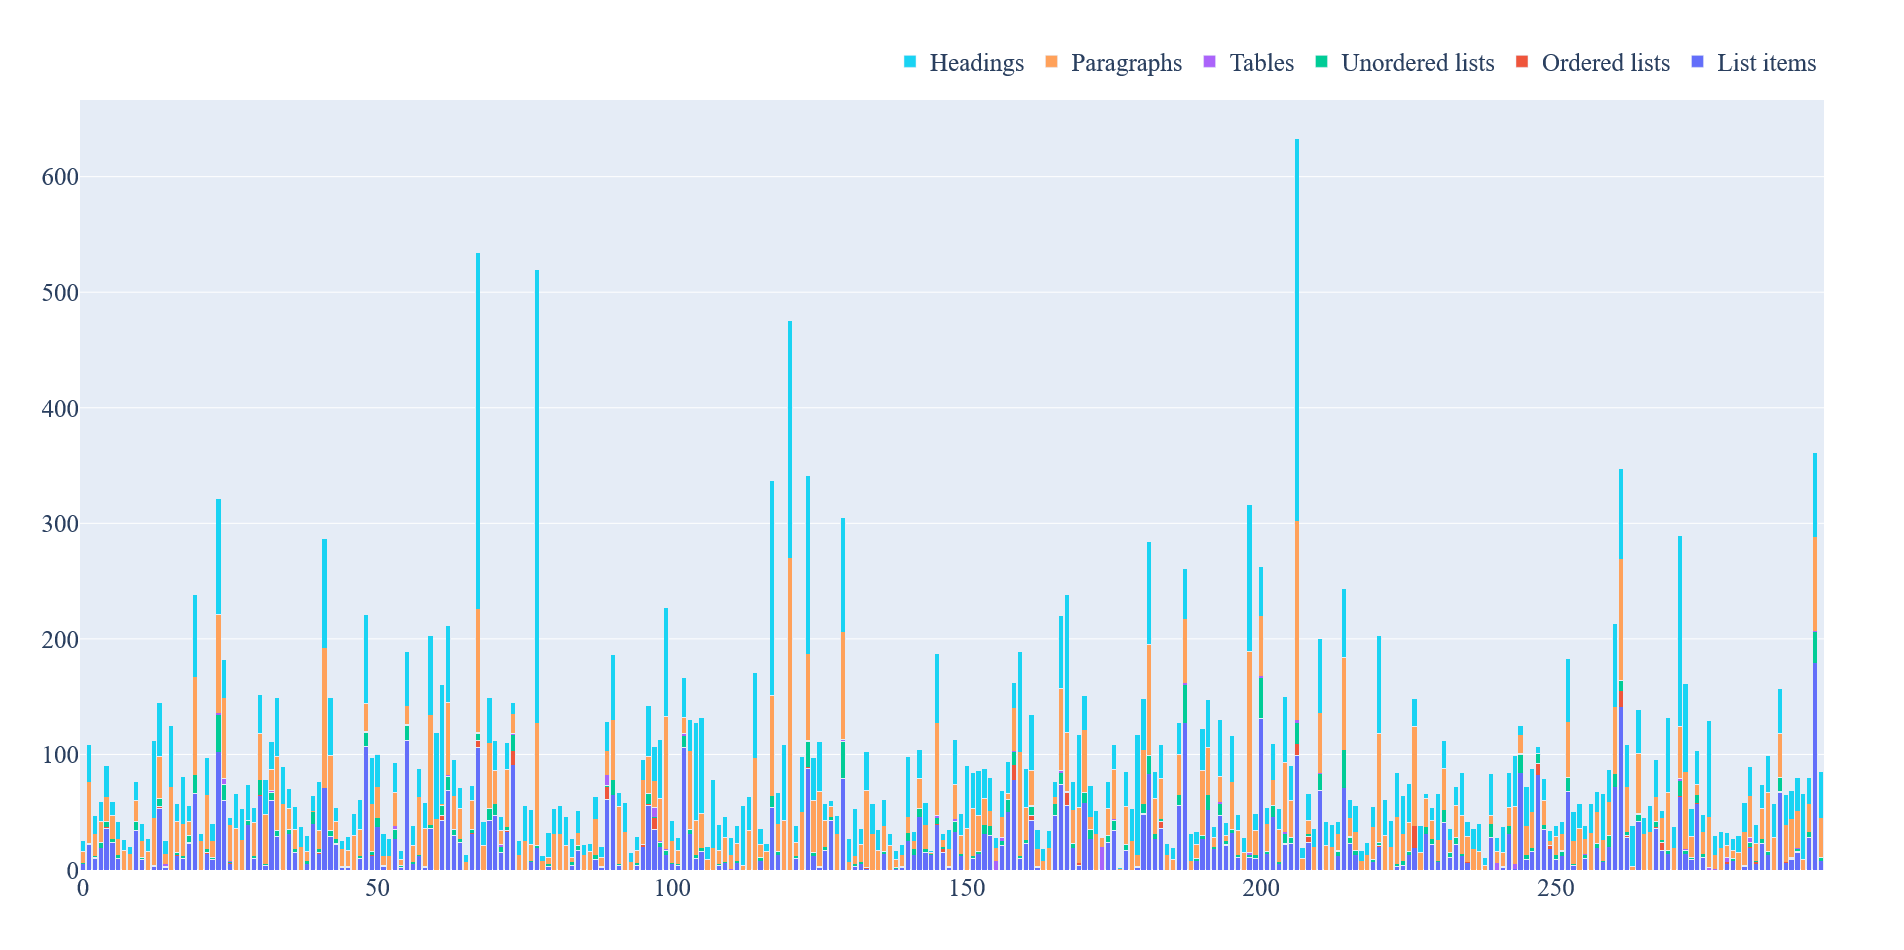
\includegraphics[width=\textwidth]{structure_stats2.png}}
    \vspace{-\baselineskip}
\end{figure}

Таким образом можно описать среднестатистическую политику безопасности, которая состоит из 31.5 абзацев, 33 заголовков, 23.6 элементов перечислений, 0.7 нумерованных списков, 4.4 ненумерованных списка, 0.5 таблиц.

Для дополнительного статистического анализа дата сета, он был кластеризован с помощью латентного размещения Дирихле. Как и в [-] для кластеризации политики безопасности были разбиты на абзацы, после чего была проведена предобработка, состоящая из лемматизации и удаления пунктуации и так называемых <<стоп слов>>. В таблице \ref{tab:iot_clusters} приведены результаты моделирования тем в IoT дата сете. В [-] уже была исследована точность латентного размещения Дирихле, его преимущества и недостатки, на основании чего IoT дата сет был проанализирован именно таким способом.  По ним видно, что с помощью такой кластеризации можно выделить различные аспекты политик безопасности.

\begin{ltwrap}{2mm}{1.7}{\footnotesize}
    \begin{longtable}[H]{|C{.05\x}|M{.475\x}|M{.475\x}|}
        \caption{Тематическое моделирование\label{tab:iot_clusters}}\\\hline
        \multicolumn{1}{|H{.05\x}|}{№}
        & \multicolumn{1}{H{.475\x}|}{Координаты семантическогопространства} 
        & \multicolumn{1}{H{.475\x}|}{Возможные сценариииспользования}\\\hline
        \endfirsthead
        \caption*{Продолжение таблицы \ref{tab:iot_clusters}}\\\hline
        \multicolumn{1}{|H{.05\x}|}{№}
        & \multicolumn{1}{H{.475\x}|}{Координаты семантическогопространства} 
        & \multicolumn{1}{H{.475\x}|}{Возможные сценариииспользования}\\\hline
        \endhead
        \endfoot
        \endlastfoot
        0 & email, send, promotional, communication, marketing, opt, product, service, message, list & First-party collection, Opt-in, opt-out messages and notifications to end user \\\hline
        1 & party, third, service, information, privacy, website, share, policy, site, advertising & Third parties sharing for marketing purposes \\\hline
        2 & removed, href, hyperref, question, contact, privacy, us, please, policy, comment & Contact information: company \\\hline
        3 & cookie, device, browser, service, address, website, site, collect, information, use & First-party collection: browser and device information \\\hline
        4 & child, age, entering, detection, year, fill, redirected, show, knowingly & Special audience: children \\\hline
        5 & sensor, educational, suggestion, top, acquirer, mailing, employment, job, taking, clickstream & First-party collection: device and service specific information \\\hline
        6 & corporate, automated, storefrontdigest, indefinite, personalization, direction, administrator, token, shop, employed & Other \\\hline
        7 & data, personal, right, request, processing, information, necessary, legal, purpose, law & First-party collection: right to edit, access, with specified (legal) basis of data processing \\\hline
        8 & sponsor, push, reply, default, swiss, desire, becoming, correspondence, calling, representative & Other \\\hline
        9 & asset, service, product, merger, company, item, list, business, another, referral & Third-party sharing in case of company acquisution and merging \\\hline
        10 & erasure, unaffiliated, input, approximate, format, appliance, pref, persistent, canadian, short & Right to erase \\\hline
        11 & address, name, information, account, email, promotion, password, u, collect, contact & First-party collection: personal and account information \\\hline
        12 & security, protect, safety, hosted, secure, violate, property, others, technical, law & Data security \\\hline
        13 & california, state, resident, institution, law, united, ccpa, right, request, country & Special audience: California residents \\\hline
        14 & change, policy, privacy, statement, time, notice, pci, payment, ds, update & Privacy policy changes \\\hline
    \end{longtable}
\end{ltwrap}

На рисунке 7 приведены результаты кластеризации дата сета. При кластеризации порог аффилиации абзаца политики безопасности был установлен в 0.3, параграф относился к нескольким кластерам, если вероятность аффилиации с ним была больше указанного порога. По графику на рисунке \ref{fig:topics_stats} можно судить, какую часть от общего объема текстов занимают те или иные аспекты политик безопасности.

\begin{figure}[H]
    \centering
    \ffigbox[\FBwidth]
    {\caption{Статистика аспектов в IoT дата сете\label{fig:topics_stats}}}
    {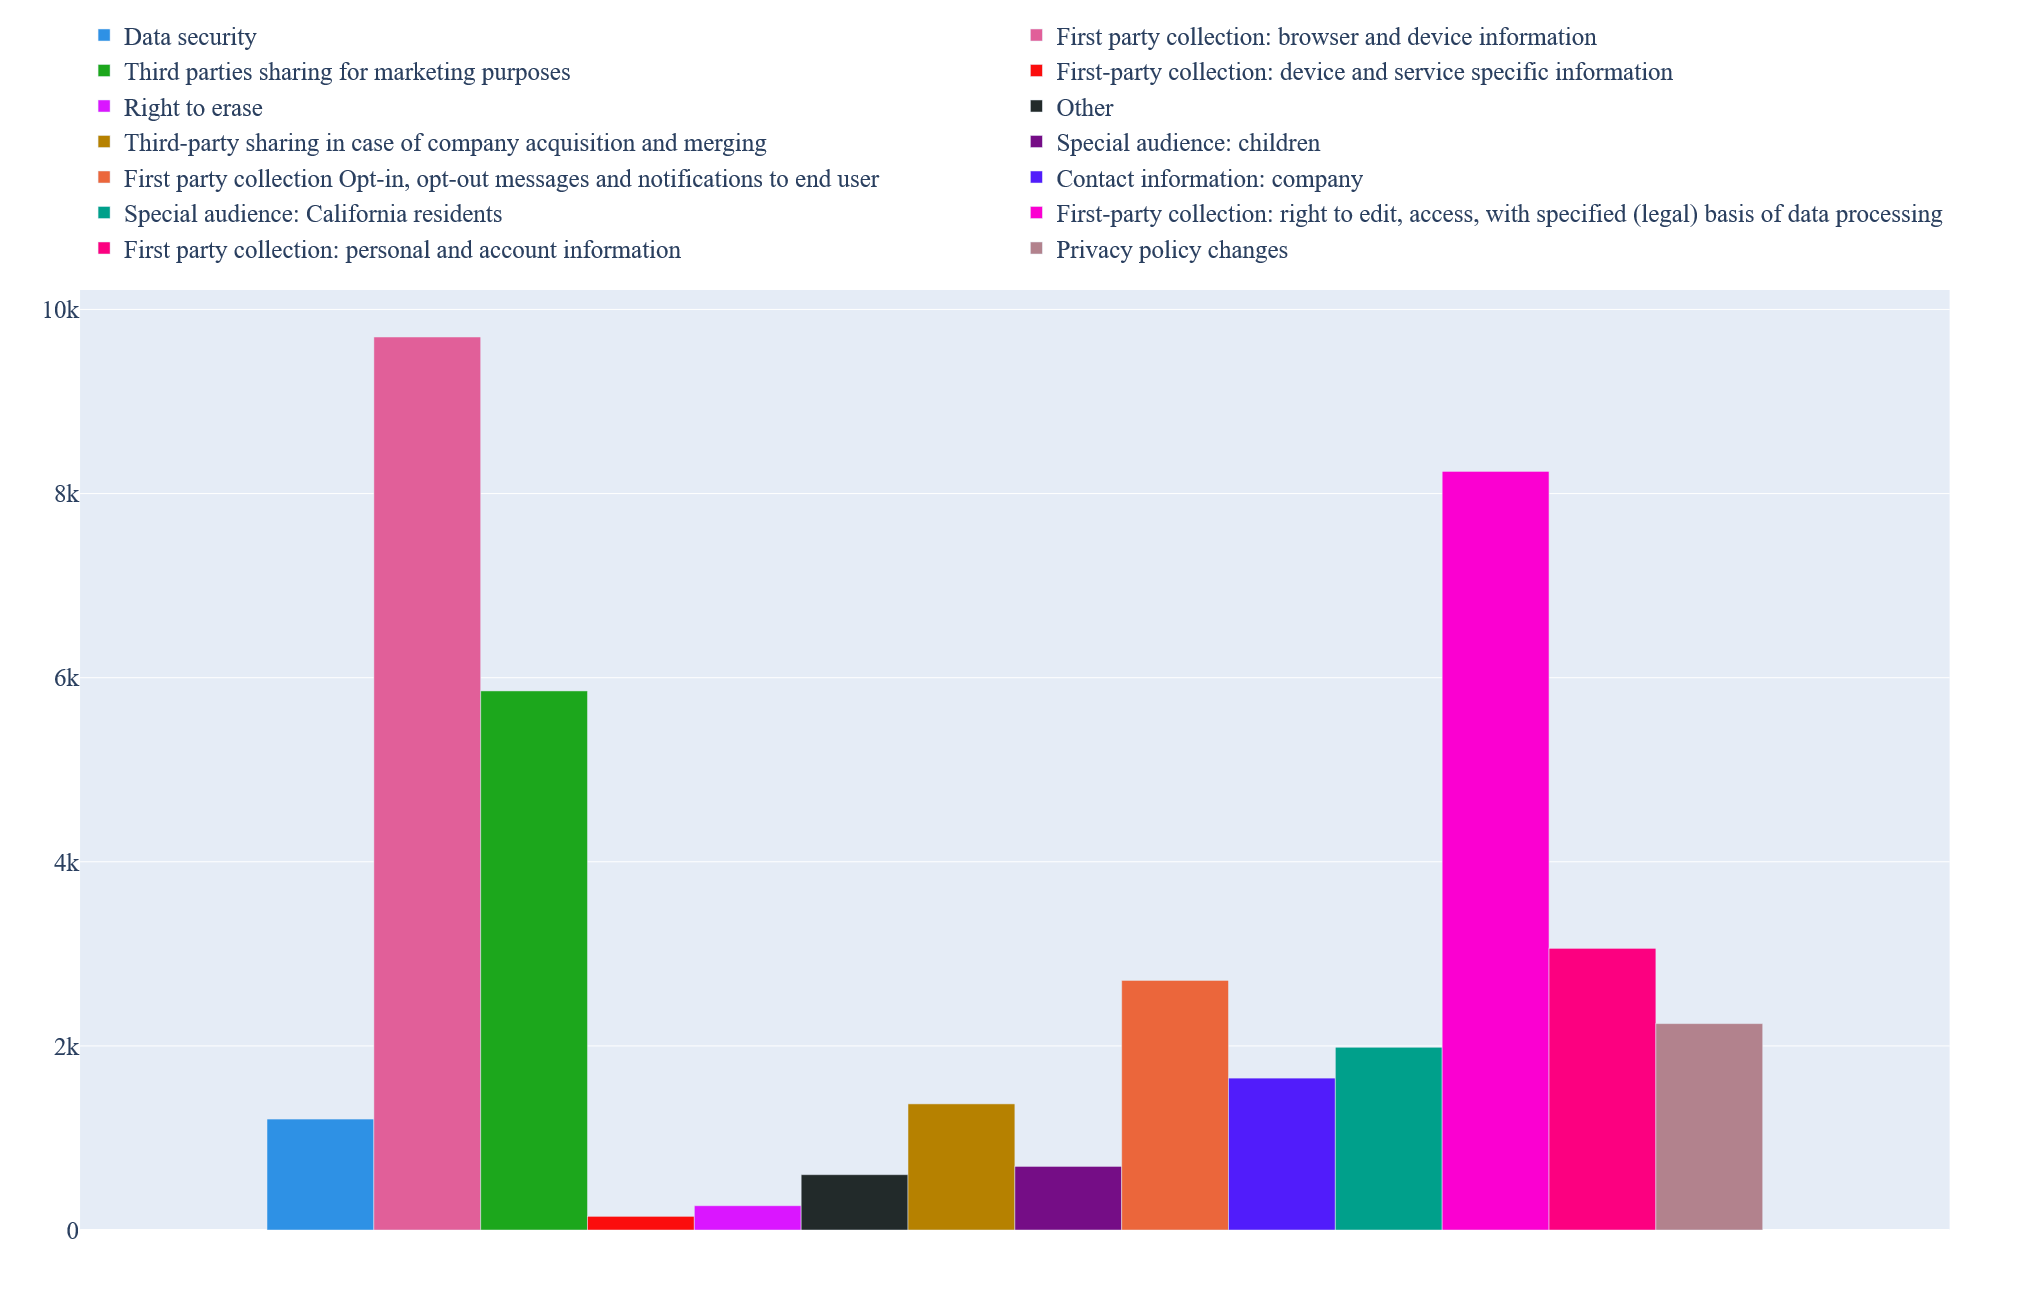
\includegraphics[width=\textwidth]{topics_stats.png}}
    \vspace{-\baselineskip}
\end{figure}

Как заключение статистического обзора сформированного дата сета на рисунке \ref{fig:topics_stats1} и \ref{fig:topics_stats2} приведено детальное распределение аспектов политик безопасности по каждой конкретной политике. Здесь в виде гистограммы представлены распределения всех 15 аспектов, выделенных алгоритмом LDA. Каждый абзац может относиться к нескольким аспектам с порогом аффилиации 0.3.

\begin{figure}[H]
    \centering
    \ffigbox[\FBwidth]
    {\caption{Статистика первых 246 политик в IoT дата сете по аспектам\label{fig:topics_stats1}}}
    {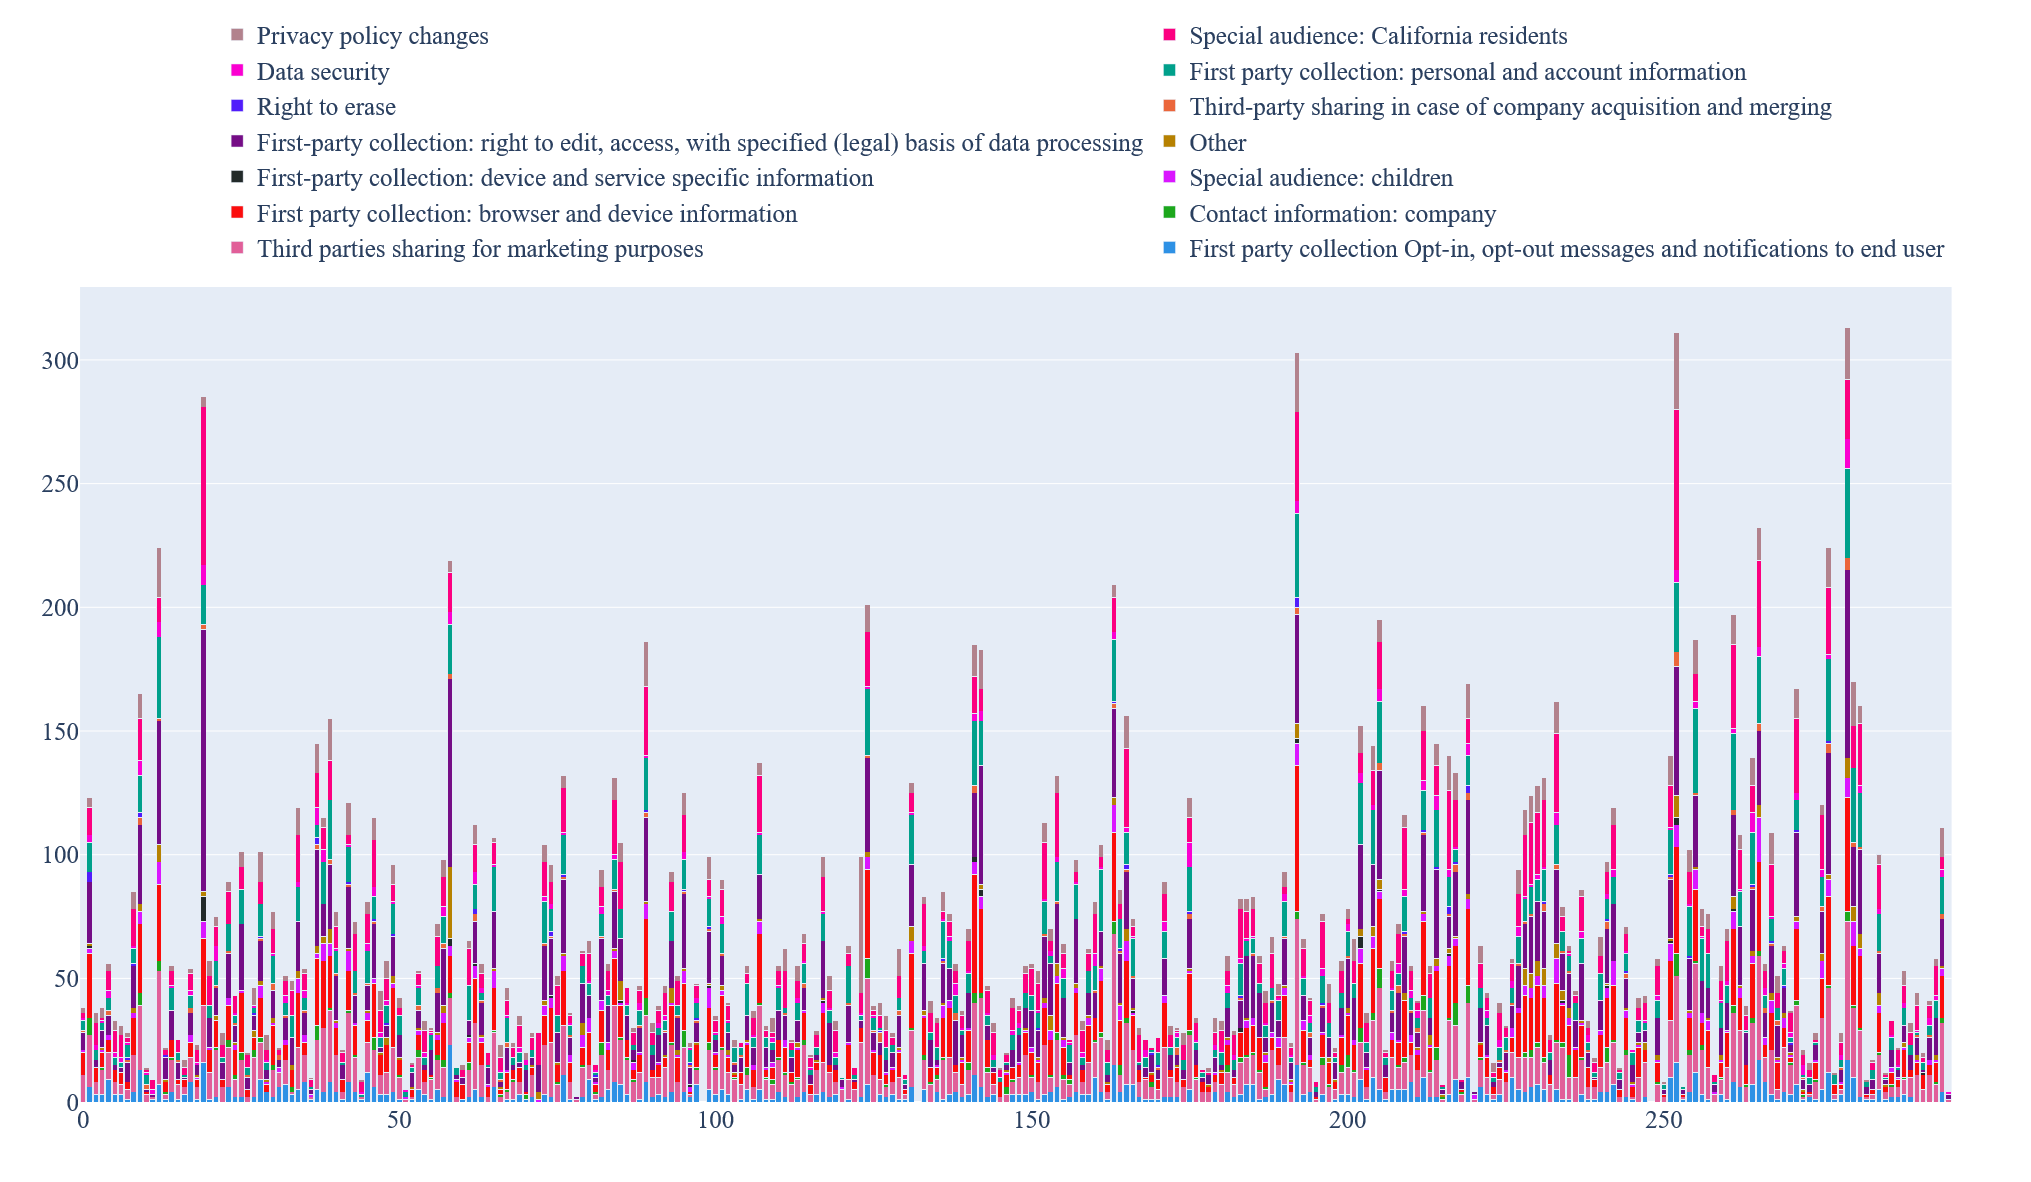
\includegraphics[width=\textwidth]{topics_stats1.png}}
    \vspace{-\baselineskip}
\end{figure}

\begin{figure}[H]
    \centering
    \ffigbox[\FBwidth]
    {\caption{Статистика последних 246 политик в IoT дата сете по аспектам\label{fig:topics_stats2}}}
    {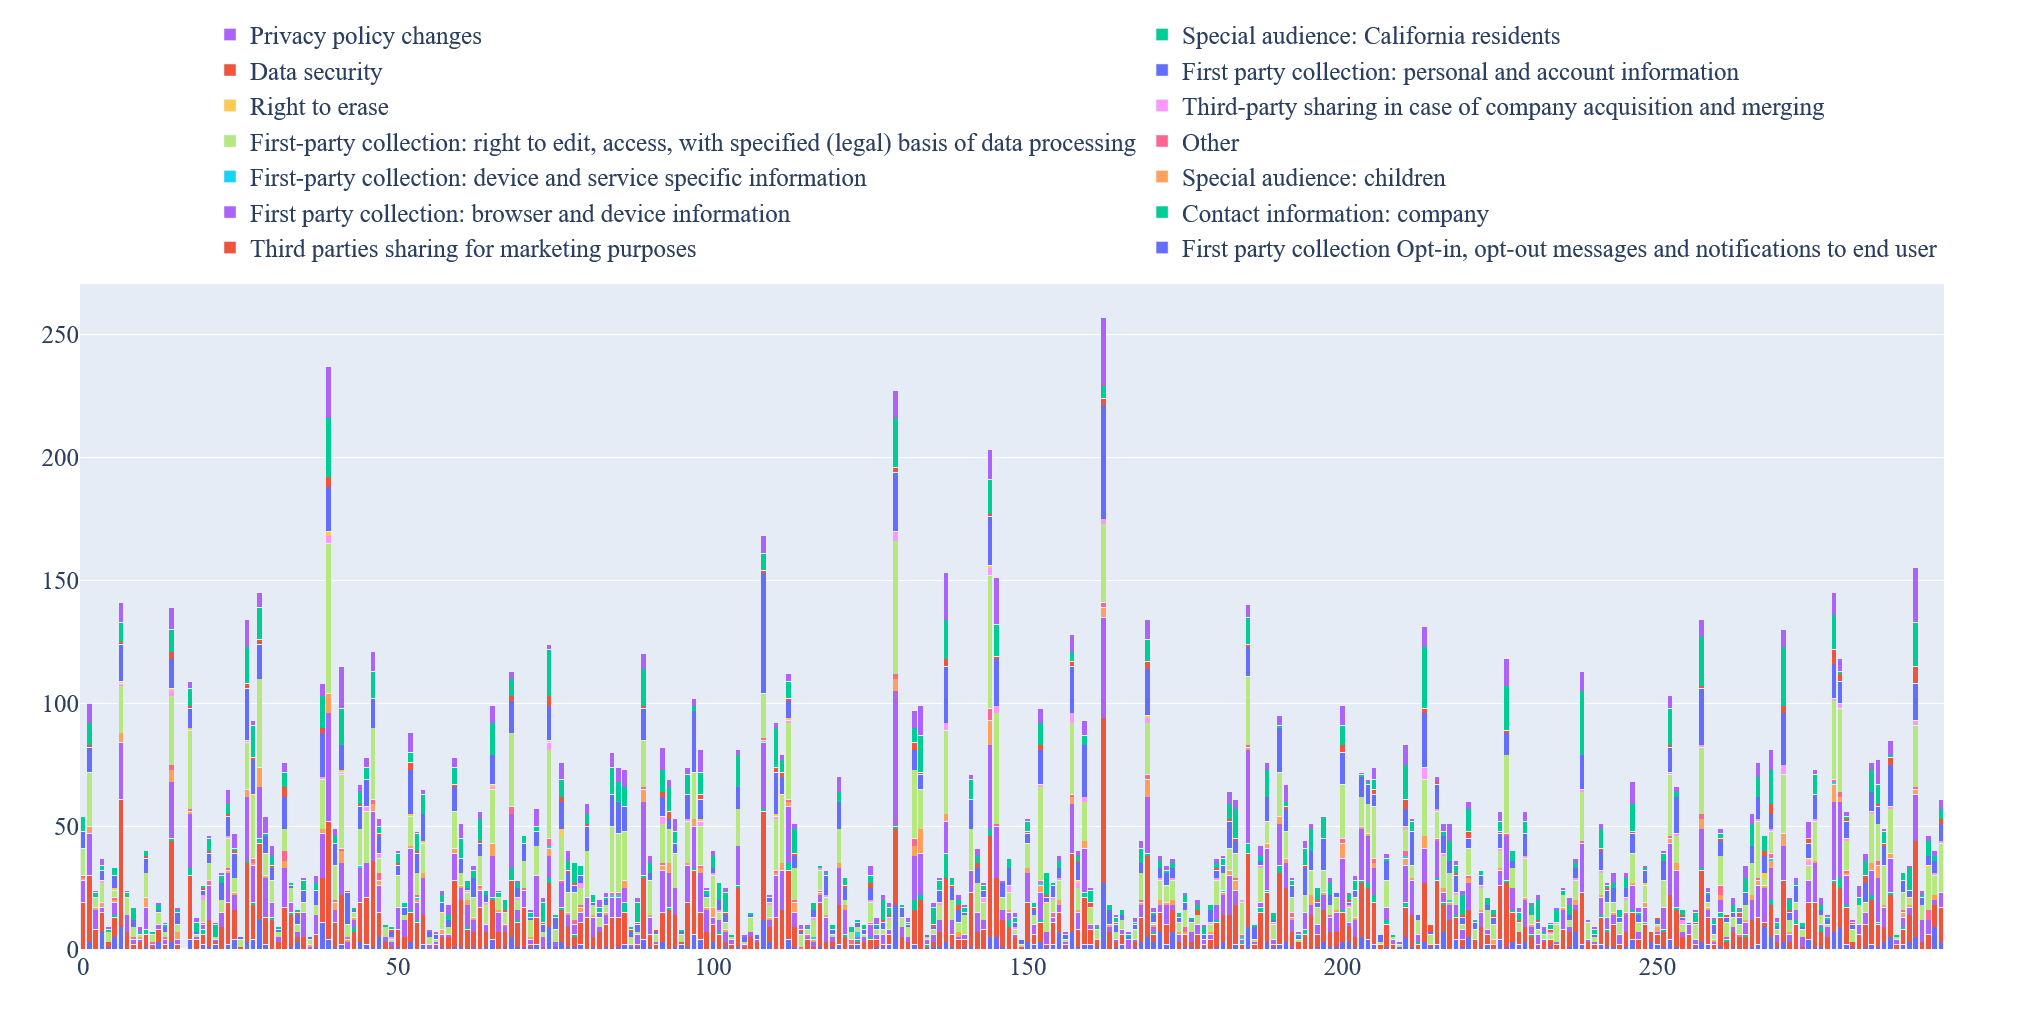
\includegraphics[width=\textwidth]{topics_stats2.png}}
    \vspace{-\baselineskip}
\end{figure}

\subsection{Полученный в результате реализации инструмент разметки}
Текст\dots

\subsection{Результаты решения поставленной задачи с помощью разработанного инструментария}
Текст\dots

\newpage
\section{Составление бизнес-плана по коммерциализации результатов научно-исследовательской работы магистранта}
Текст\dots

\end{document}